%%%%%%%%%%%%%%%%%%%%%%%%%%%%%%%%%%%%%%%%%%%%%%%%%%%%%%%%%%%%%%%%%%% 
%                                                                 %
%                            ROOT FILE                            %
%                                                                 %
%%%%%%%%%%%%%%%%%%%%%%%%%%%%%%%%%%%%%%%%%%%%%%%%%%%%%%%%%%%%%%%%%%% 
%
%  Run LaTeX or pdfLaTeX on this file to produce your thesis.
%  To produce the abstract title page followed by the abstract,
%  see the file abstitle-phd.tex or abstitle-mas.tex.
%
%%%%%%%%%%%%%%%%%%%%%%%%%%%%%%%%%%%%%%%%%%%%%%%%%%%%%%%%%%%%%%%%%%%

\documentclass[chap]{thesis}
\usepackage{physics}
\usepackage{amssymb}
\usepackage{amsmath}
\usepackage{bm}
\usepackage{subcaption}
\usepackage{indentfirst}
%\usepackage{newpxtext,newpxmath}
\usepackage{multirow}
\usepackage{tabularx}
\usepackage[hidelinks]{hyperref}
\newcommand{\angstrom}{\text{\normalfont\AA}}


% Uncomment the following if you want centered-lined captions:
%\captionsetup{format=plain,justification=centering}


%\includeonly{preface}  % use \includeonly to process only
%\includeonly{introduction,hydration}
                         % the file(s) listed inside the braces        
\begin{document}
 
% Use the appropriate example title page.  A senior thesis
% can be set by changing the thesis name in rpititle-mas.tex. 
%%%%%%%%%%%%%%%%%%%%%%%%%%%%%%%%%%%%%%%%%%%%%%%%%%%%%%%%%%%%%%%%%%% 
%                                                                 %
%                            TITLE PAGE                           %
%               Master's Thesis or Master's Project               %
%                                                                 %
%%%%%%%%%%%%%%%%%%%%%%%%%%%%%%%%%%%%%%%%%%%%%%%%%%%%%%%%%%%%%%%%%%% 
%  This file produces the title page, copyright page (if requested)
%  and the Table of Contents, List of Figures and List of Tables.
% 
%  To produce the abstract title page followed by the abstract,
%  see the template file, "abstitle-mas.tex"
%%%%%%%%%%%%%%%%%%%%%%%%%%%%%%%%%%%%%%%%%%%%%%%%%%%%%%%%%%%%%%%%%%%

% Supply information for use on title page:    
\thesistitle{\bf On the Interactions of Water with Montmorillonite Clay Minerals}        
\author{Hunter Christophe Belanger}        
\degree{Master of Science} 
\department{Physics} % provide your area of study here; e.g.,
%  "Mechanical Engineering", "Nuclear Engineering", "Physics", etc.
   
\signaturelines{3}
\thadviser{Dr. Ingrid Wilke} % For a masters project use \projadviser instead of \thadviser,
\memberone{Dr. Gyorgy Korniss}        
\membertwo{Dr. Humberto Terrones}
%\memberthree{Aristotle} % must change signaturelines to 4 if using this 4 members

\submitdate{[May 2019]\\Submitted March 2019}        
\copyrightyear{2019}   % if omitted, current year is used.        

% Print titlepage and other prefatory material:   
\titlepage     
\copyrightpage         %optional           
\tableofcontents        
\listoftables          %required if there are tables
\listoffigures         %required if there are figures

   % titlepage material for Master thesis p
%%%%%%%%%%%%%%%%%%%%%%%%%%%%%%%%%%%%%%%%%%%%%%%%%%%%%%%%%%%%%%%%%%% 
%                                                                 %
%                         ACKNOWLEDGEMENT                         %
%                                                                 %
%%%%%%%%%%%%%%%%%%%%%%%%%%%%%%%%%%%%%%%%%%%%%%%%%%%%%%%%%%%%%%%%%%% 
 
\specialhead{PREFACE}
 
During my second year at RPI as an undergraduate, I began a research project with my current advisor, Professor Wilke, on the X-ray diffraction of montmorillonite clay samples. As a young aspiring physicist, I must admit that studying clay minerals was not high on my list of interests. That summer however, I was given a workbench in a chemistry lab, an assortment of various chemicals, and access to a very cool X-ray diffractometer. This mixture of excitement to begin using the diffractometer and pure fear of poisoning myself was an interesting feeling to say the least. As I began performing measurements and coming up with my first experiments, the fear subsided and I started to enjoy going to the lab, carrying a tray full of clay samples to the diffractometer, and spending several hours watching Bragg peaks form on a computer screen.

After that summer, I decided that looking at clay for the time being wasn't as odd or as boring as my parents initial reaction to hearing my research topic would have implied. I decided to keep working with Professor Wilke, who had a new experiment in mind for me, collecting infrared spectra of montmorillonite samples. My research in this field continued through my undergrad, until it became my graduate research as well, as I completed my Masters degree. After almost four years of working on a subject, you begin to acquire a large bit of knowledge and data on a topic. It is for this reason, and the fact that I desired to pursue my PhD in Europe, that Professor Wilke encouraged me to complete a Masters Thesis, in lieu of a Masters Project which is far more common in the Physics department. I was skeptical at first, as a thesis seemed like much more work than a project, and finishing a Masters degree in one year already seemed like it would be difficult enough. She insisted that I had enough work to produce a thesis, and that it would help me for when I have to write my Doctoral Thesis later on.

These seemed like valid reasons, so I followed her advice and opted for the thesis. As soon as I began writing this manuscript however, I realized that I had been right about something; writing a thesis is very difficult. The beginning was painfully slow, and the perpetual ignorance of not knowing where to even begin postponed its initiation. Once I had written my first chapter however, it started to become much easier to continue. I would find myself easily working until the early morning hours on the weekend, not realizing how much time had actually gone by. To a fair extent, I began to enjoy it. In addition, it was clear that I had learned a lot about the writing process, and also more about my research as a whole as I was forced to think about it in a new manner. This thesis has made me a better physicist, and better prepared me to go out, and begin work on a PhD. I cannot thank Professor Wilke enough for her encouraging me to complete a thesis, for without her advice this work would likely not exist, and I would not be as well prepared as I am today. To other young physicists reading this, I encourage you to do the same, as it will certainly make you a better scientist, and only better prepare you for the future, whether you plan on doing a PhD afterwords or not.
\newline
\begin{flushleft}

\includegraphics[scale=0.2]{images/signature.png}\newline
Hunter Belanger
\newline\newline
Troy, New York\newline
March, 2019
\end{flushleft}

%%%%%%%%%%%%%%%%%%%%%%%%%%%%%%%%%%%%%%%%%%%%%%%%%%%%%%%%%%%%%%%%%%% 
%                                                                 %
%                         ACKNOWLEDGEMENT                         %
%                                                                 %
%%%%%%%%%%%%%%%%%%%%%%%%%%%%%%%%%%%%%%%%%%%%%%%%%%%%%%%%%%%%%%%%%%% 
 
\specialhead{ACKNOWLEDGMENT}
Many people have helped to bring this thesis to fruition, and must be recognized. First are collaborators Michael Aldersley and Prakash Joshi who helped prepare the samples used through the course of this work, and have provided much advice through the course of this research project over the past few years. I would also like to thank some of our collaborators at Corning Inc, particularly Aravind Rammohan and Ross Stewart, with whom I have had many fruitful conversations, and who helped with starting the molecular dynamics simulations. Another priceless resources through this project was Siddharth Sundararaman, who was instrumental in getting the molecular dynamics simulations off the ground.

There are many people in my life who have played a large role in my success at RPI, and helped me complete this thesis. I would first like to thank all of my friends here at RPI who have made the stressful school life here far more palatable. Without all of you, I would have surely gone crazy, and the long nights working on homework would have been far longer.

Great appreciation is also extended to the French department at SUNY Albany for being so accepting and accommodating in the many French classes which I took there during my time at RPI. A special thanks is extended Professor Susan Blood, who helped foster and encourage my learning in French language and literature, and with whom I was able to spend many hours conversing on topics in French history and literature. Without these experiences, I would be far less prepared to begin further studies in France than I am now.

Next are my parents who have put up with my perpetually being away from home for most of the past five years. Their encouragement, and love however has been an absolutely critical component in the completion of this work. I also thank them for their further acceptance of my being away from home, as I prepare to move abroad for my PhD.

Lastly, I would like to thank the Physics department here at RPI. All of the professors have been the leading instrument in my formation as a physicist thus far. This is especially true of Professor Wilke, who has supported, encouraged, instructed, and advised me over the past five years. I will truly miss our hours of discussion on my research and various other topics. Her advice in preparing this manuscript and applying to graduate schools has been more than instrumental in helping me achieve my goals, and I cannot thank her enough.  % include for acknowledgements
%%%%%%%%%%%%%%%%%%%%%%%%%%%%%%%%%%%%%%%%%%%%%%%%%%%%%%%%%%%%%%%%%%% 
%                                                                 %
%                            ABSTRACT                             %
%                                                                 %
%%%%%%%%%%%%%%%%%%%%%%%%%%%%%%%%%%%%%%%%%%%%%%%%%%%%%%%%%%%%%%%%%%% 
 
\specialhead{ABSTRACT}

The topic of this thesis is an infrared spectroscopic study of water intercalated in layered silicates as a function of pH. This is important due to the catalytic properties of phyllosilicate clay minerals such as montmorillonite, which have a known dependence on the pH of the system, and the amount of water intercalated in the clay. This could improve our understanding of the catalysation mechanism at play, and the interactions of water at the nanoscale.

For this purpose, a simple method to control the hydration of montmorillonite clay samples was investigated, using saturated salt solutions to control the relative humidity of the storage environment. Samples of montmorillonite were placed in desiccators with different solutions in the base, controlling the ambient moisture level around the samples. X-ray diffraction was used to measure the basal spacing of the samples, indicating the number of layers of water present between clay sheets. It was found that samples in the form of compressed pellets were much more difficult to hydrate than clay powder. The working time outside of the humid environment was also found to be on the order of just minutes, before the clay returns to a lesser hydrated state. 

Infrared spectroscopy was used to investigate the pH dependence of the vibrational modes of water intercalated in the clay. Spectra of montmorillonite with exchangeable cation species of either Li, Na, or K, from differing origin clay mines were collected at pH values between 3 and 10. For all investigated exchangeable cations and clay mines, it was observed that the frequency of the symmetric stretching mode increased as the pH of the system increased. No significant changes in frequency were observed in the water deformation mode, or the O-H stretching mode of the structural hydroxyl groups in the clay.

Subsequently, a model to perform molecular dynamics simulations of the clay-water interface was developed for the interpretation of the experimental data. Using the InterfaceFF suite provided montmorillonite structures were combined with the flexible water model. This allowed for a basic simulation of the water vibrational modes. An algorithm for determining the frequency of these vibrational modes using Fourier transforms on the atom positions is also proposed. Simulations conducted using this system had water vibrational modes similar to those of the experimentally observed frequencies. % abstract
%%%%%%%%%%%%%%%%%%%%%%%%%%%%%%%%%%%%%%%%%%%%%%%%%%%%%%%%%%%%%%%%%%% 
%                                                                 %
%                            ABSTRACT                             %
%                                                                 %
%%%%%%%%%%%%%%%%%%%%%%%%%%%%%%%%%%%%%%%%%%%%%%%%%%%%%%%%%%%%%%%%%%% 
 
\specialhead{RÉSUMÉ}
 
Le sujet de cette thèse est un étude de spectroscopie infrarouge de l’eau intercalé dans les silicates en couches en fonction du pH. C’est une étude importante car les propriétés des argiles, comme le montmorillonite, ont une dépendance sur le pH du système, et la quantité d’eau intercalé dans l’argile. Cela pourrait nous donner de nouvelles connaissances sur ce mécanisme de catalysation, et les interactions d’eau à l’échelle nanométrique.

Une méthode pour contrôler l'hydratation d’échantillons d’argile montmorillonite a été examinée. Les solutions de sel saturées maintiennent l'humidité dans un espace clos. Les échantillons ont été mis dans un dessiccateur, avec la solution de sel saturée qui maintenait une humidité prévue. La diffractométrie de rayons X a été utilisée afin de mesurer l’espace entre les feuillets d’argile, qui est déterminé par la quantité d’eau intercalé, c’est-à-dire le nombre de strates d’eau entre deux feuillets. Les échantillons d’argile de la forme d’un disque comprimé étaient plus difficile à hydrater que l’argile en poudre. C’était aussi évident que l’on n’aurait que quelques minutes pour travailler avec l’échantillon en dehors du dessiccateur avant qu’il ne se retrouve dans un état moins hydraté.

La spectroscopie infrarouge a été employée pour analyser la dépendance du pH sur les fréquences des vibrations moléculaires de l’eau intercalé dans l’argile. Les spectres des échantillons avec des espèces de cations échangeables différents, et venant de mines différentes, ont été obtenus avec des pH entre 3 et 10. Pour chaque cation et mine considéré, la fréquence de l’étirement symétrique d’eau augmentait avec le pH. Il n’y avait pas de changement dans la fréquence de cisaillement d’eau, ni dans la fréquence de l’étirement de la liaison O-H des hydroxyles de l’argile.

Puis, un modèle pour simuler ce système avec la dynamique moléculaire a été réalisé. Utilisant la suite de InterfaceFF, les structures de montmorillonite inclus ont été combinées avec le modèle d’eau flexible. Cela a permit la simulation des vibrations dans les molécules d’eau. Pour obtenir la fréquence de chaque vibration, une transformation de Fourier a été faite sur les positions des atomes, permettant l'obtention des fréquences des vibrations de l’eau. Ces fréquences étaient proche de celles déjà obtenues lors des expériences précédentes.

 
 % abstract in Fr.
%%%%%%%%%%%%%%%%%%%%%%%%%%%%%%%%%%%%%%%%%%%%%%%%%%%%%%%%%%%%%%%%%%% 
%                                                                 %
%                            CHAPTER ONE                          %
%                                                                 %
%%%%%%%%%%%%%%%%%%%%%%%%%%%%%%%%%%%%%%%%%%%%%%%%%%%%%%%%%%%%%%%%%%%
\chapter{Introduction}
\section{Motivation}
Phyllosilicate clay minerals such as montmorillonite have been of interest to researchers of various domains for more than fifty years. Many different aspects of this material have been studied, ranging from its hydration and swelling properties \cite{aldrich1944hydration}, to its chemical properties, such as catalyzing the formation of RNA oligomers \cite{joshi2009mechanism}. Being a safe, naturally occurring material, it has found a wide variety of uses such as in pharmaceuticals, cosmetics, and oil refining \cite{hartwell1965diverse}.

Having found such a plethora of uses, its maintained interest over the years is understandable. As previously mentioned, a main industrial use for the material is its use as a catalyst for chemical reactions \cite{hartwell1965diverse}. More recently however, these known catalytic properties have expanded to include the catalyzation of RNA oligomers as expanded by Prakash Joshi, Michael Aldersley, John Delano, and James Ferris here at Rensselaer Polytechnic Institute (RPI) \cite{joshi2009mechanism}, \cite{aldersley2011role}. In addition to this fact, montmorillonite has also been shown to help catalyze the formation of vesicles from fatty acid micelles as shown by Hanczyc, Fujikawa, and Szostak \cite{hanczyc2003experimental}. The combination of these two catalytic capabilities has increased the interest of montmorillonite amongst biochemists and has incorporated montmorillonite into some theories of abiogenisis, as a possible candidate for having been the catalyst for the first protocells, and precursors of life on Earth \cite{hanczyc2003experimental}.

The conditions allowing montmorillonites to maximize their catalytic properties in terms of RNA oligomer formation has been previously researched \cite{aldersley2011role}, \cite{aldersley2011evaluation}, but much is still unknown about the exact physics and chemistry governing these processes. Its importance in industrial applications, as well as to the theory of abiogenisis in conjunction with this lack of basic understanding behind the underlying principles is what has prompted this research.

\section{Background and Previous Works}
\subsection{Structure of Montmorillonite}
Montmorillonite is the most prominent form of smectite, which is in turn a type of phyllosilicate. The most basic structure of montmorillonite is a sheet formed by two tetrahedral sheets which sandwich a dioctahedral sheet \cite{sposito1984surface}. Such a structure is referred to as a 2:1 structure, in reference to being composed of two tetrahedral sheets and one dioctahedral sheet. The tetrahedral sheets are in general composed of silica, with aluminum substitutions, and the dioctahedral sheet is alumina which may also be substituted by iron and magnesium. In all, the chemical formula for montmorillonite is given as
\begin{equation*}
	[(Si_{3.88}Al_{0.12})^{IV}(Al_{1.64}Fe_{0.05}^3Mg_{0.36})^{VI}O_{10}(OH)_2]_2
\end{equation*}
where the superscripts $IV$ and $VI$ refer to the coordination of the tetrahedral and dioctahedral structures respectively \cite{van1977introduction}. A diagram of these structures is presented in Figure ~\ref{fig:clay_structure}.
\resetfootnote
\begin{figure}
	\centering
	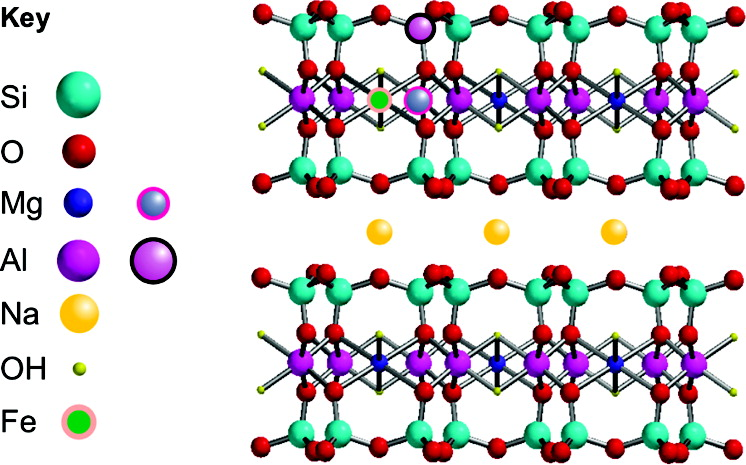
\includegraphics[scale=1.75]{images/clay_structure.jpg}
	\caption{Diagram of montmorillonite unit cell\protect\footnotemark. Outlined atoms indicate substitutions \cite{joshi2009mechanism}.}
	\label{fig:clay_structure}
\end{figure}
\footnotetext{ Reprinted with permission from P.C. Joshi, M.F. Aldersley, J.W. Delano, and J.P. Ferris, “Mechanism of montmorillonite catalysis in the formation of RNA oligomers,” \textit{J. Amer. Chem. Soc.}, vol. 131, no. 37, pp. 13 369–13 374, Sept. 2009. Copyright 2009 American Chemical Society.}

The substitutions in the clay cause a buildup of a net negative charge on the surfaces of the clay structure due to the provided supplemental electrons. The magnitude of this charge depends on the number and type of substitutions. Due to these variations, different types or varieties of montmorillonite are known to have different surface charges. This value can range from 0.66 to 0.98 per O$_{20}$(OH)$_4$ formula unit \cite{joshi2009mechanism}, \cite{newman1987chemical}. As the Coulomb force between sheets of clay would naturally repel them, positively charged exchangeable interlaminar cations are present between the sheets, leading to a net neutral charge and neutralizing the repulsive force between sheets \cite{mering1953role}. Typically, these cations are alkali or alkaline earth metals such as Na, Li, K, Mg, or Ca \cite{berend1995mechanism}. For the work conducted within this thesis, only montmorillonite samples with interlaminar cations of Li, Na, and K were used.

\subsection{Swelling Properties}
In a completely dry sample of montmorillonite, the interlaminar cations are located in the hexagonal cavities on the external surfaces of each individual clay sheet. For Na montmorillonite, this results in a basal spacing between sheets of approximately $d_{001}=9.6\angstrom$ \cite{cases1992mechanism}. This spacing for dry montmorillonites is dependent on the valence or radius of the exchangeable cation of the particular sample in question \cite{mering1953role}. While both Li and Na montmorillonites have a basal spacing of approximately 9.6$\angstrom$, it is found that this value increases to 9.95$\angstrom$ for K, 10.25 - 10.6$\angstrom$ for Rb, and 10.7 - 11.5$\angstrom$ montmorillonites \cite{berend1995mechanism}.

Water in the vicinity of montmorillonite has the tendency to be absorbed by the mineral. These water molecules may accumulate on the surfaces of the clay structure, but are also intercalated between the clay sheets, solvating the exchangeable cations \cite{aldrich1944hydration}, \cite{mering1946hydration}. During this process, the cations will be unseated from the hexagonal cavities, and be more freely accessed by the intercalated water \cite{mering1953role}. Upon sufficient water content, usually provided in the form of water vapor from the ambient atmosphere, a monolayer of water will form between the clay sheets. Increasing the availability of water (by increasing the relative humidity in most cases) will eventually facilitate the formation of a bilayer of water, and subsequently a trilayer and so on. With each added layer of water, the basal spacing between sheets also increases. The type of exchangeable cation which is present in the clay will dictate these spacings, as well as how many layers of water may form \cite{mering1964gonflement}.

Often, it is possible to achieve up to three layers of water between sheets for Li, and Na montmorillonite. For K montmorillonite however, it is difficult to obtain a bilayer and for cations with a valence larger than this, such as the cases with Cs and Rb, only a monolayer is possible \cite{mering1964gonflement}. Spacings for a monolayer of water are usually in the vicinity of $d_{001}=12.0\angstrom$ for Li, and $d_{001}=12.5\angstrom$ for Na, K, Rb, and Cs exchanged montmorillonites. A bilayer hydrate is represented by a basal spacing of $d_{001}=15.5$ - $16.0\angstrom$ \cite{berend1995mechanism}. Trilayers typically present with $d_{001}\approx 18.1\angstrom$ \cite{cases1992mechanism}. The relative humidity required to obtain a certain number of water layers between clay sheets is highly dependent on the exchangeable cation. For example, it has been shown that a sample of Na montmorillonite kept at a relative humidity of $p/p_0=0.98$, has a basal spacing of $d_{001}=15.76\angstrom$. Similarly prepared K montmorillonite kept at a humidity of $p/p_0=0.97$ for more than four times as long as the Na sample was found to have a basal spacing of only $d_{001}=12.08\angstrom$ \cite{berend1995mechanism}. Jacques Méring and Rachel Glaeser were also able to show that it is easier to hydrate a montmorillonite which has exchangeable cations of a higher valence (such as Ca$^{2+}$), as the non-local charge cancellation increases the energy of the system, making it easier to solvate these cations \cite{mering1953role}.

A final aspect of the swelling properties of montmorillonite, which must be mentioned, is the fact that the process is very heterogeneous. By stating this, it is meant that a monolayer of water does not form homogeneously and instantly in the clay. What instead will happen is more of the interlaminar surface will be covered with a monolayer of water as the relative humidity increases, until there is a complete and homogeneous monolayer. At this point, a bilayer will begin to form as the humidity is continually increased. This process was thoroughly investigated by Cases et al. in their 1992 Langmuir paper \cite{cases1992mechanism}.

\subsection{Vibrational Modes of Intercalated Water}
Infrared spectroscopy has long been used to investigate the vibrational modes within the water molecule. For many years this methodology has been applied to investigate the specific behavior of the water which is intercalated in montmorillonite \cite{madejova2003ftir}. There are three principal vibrational modes of interest for water: symmetric O-H stretching ($\nu_1$), H-O-H bending or deformation ($\nu_2$), and asymmetric O-H stretching ($\nu_3$). One may find a depiction of these three modes in Figure~\ref{fig:water_vibrations}. It must be noted that these are all vibrations of the covalent bonds within a water molecule, and not vibrations which may occur in the hydrogen bond which forms between a hydrogen atom of one water molecule and the oxygen atom of another.

\begin{figure}
	\centering
	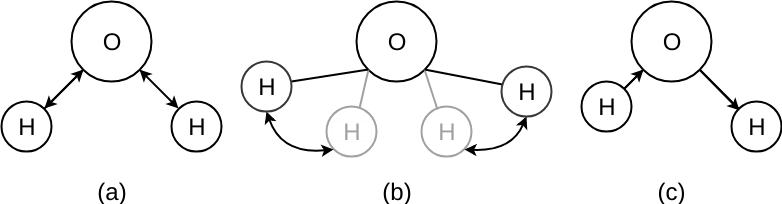
\includegraphics[scale=0.55]{images/water_vibrations.png}
	\caption{Vibrational modes of water: (a) depicts the symmetric stretching mode, (b) the bending or deformation mode, and (c) the asymmetric stretching mode.}
	\label{fig:water_vibrations}
\end{figure}

For liquid water, these modes are usually assigned frequencies of $\nu_1=3280cm^{-1}$, $\nu_2=1645cm^{-1}$, and $\nu_3=3490cm^{-1}$ \cite{eisenberg2005structure}. In liquid water, there is also an overtone of $\nu_1+\nu_2+\nu_3$ located at $3404cm^{-1}$ \cite{max2009isotope}. Although the intercalated water is in a liquid state, the frequencies of these modes are not the same as those of bulk water. The values of these frequencies for water intercalated in montmorillonite has been very well cataloged by Jana Madejová and Peter Komadel in their 2001 paper. In analyzing the infrared spectra of montmorillonite samples, they have assigned the water deformation mode to $\nu_2\approx 1632cm^{-1}$ and the stretching mode to $\nu_1\approx 3393cm^{-1}$ \cite{madejova2001baseline}. Their exact reported values vary slightly depending on location where the montmorillonite sample was taken from. A more in depth explanation of the location of these modes and the effects of exchangeable cation and hydration shall be given in chapter 3.

\section{Overview of this Work}
This thesis builds upon the already extensive body of knowledge on the subject, looking at some old problems from a new point of view, while also examining a new theory. Firstly, the hydration properties of montmorillonite were once again examined. Using X-ray Diffraction (XRD), the hydration of pressed disks of montmorillonite was examined. After being left in a desiccator at controlled humidity levels, the number of layers of water intercalated between clay sheets was measured for each disk by examining the distance between clay sheets. The goal of this experiment was to determine a simple but also effective method to accurately control the hydration of the clay samples, leaving either no water, a monolayer, bilayer, or trilayer of water between clay sheets, depending on the interlaminar cation which is present. One may find this portion of the thesis treated in chapter 2.

A novel, previously unexplored hypothesis is at the center of the second aspect of this work. The catalytic properties of montmorillonite previously discussed, have been shown to have a dependence on the pH of the clay used \cite{joshi2009mechanism}. To further explore this trend, infrared spectra of montmorillonite samples of varying interlaminar cation and pH values ranging from 3 to 10, were collected and analyzed. From the spectra of montmorillonite, one is able to observe the frequencies, and therefore corresponding energies of the O-H stretching mode, and the H-O-H deformation or "scissoring" mode of the water molecules which are intercalated. The energies of these modes were analyzed as a function of the pH of the clay, interlaminar cation, and origin of the clay sample. While infrared spectroscopy has been previously used to characterize clay minerals, no known work has been found examining pH dependencies. Due to the impact this could play on montmorillonite's ability to act as a catalyst, these results could play an important role in the fields of biochemistry and life sciences, as well as to Corning with their Life Sciences product line of laboratory glassware. This part of the research is outlined in chapter 3.

Finally, an attempt to model these montmorillonite-water surface interactions using molecular dynamics (MD) simulations was made. In this portion, two different modeling methods were attempted: one using Reax Force Fields which allow for the simulation of chemical reactions in MD simulations, and a more traditional MD approach, using standard Leonard-Jones and Coulomb potentials. Different approximations for the water molecules were also made for each of these options, where respectively the molecules were allowed to dissociate, and a flexible water model, where the O-H bonds and the angle between the two hydrogen atoms were both treated with harmonic potentials. Details pertaining to these simulations are given in chapter 4.

Also presented are considerations for future work on this subject, and future steps which are currently being considered to further examine this system, and better describe the interactions between intercalated molecules themselves, as well as with the clay surface.
 

%%% Local Variables: 
%%% mode: latex
%%% TeX-master: t
%%% End: 
 % chapter 1
%%%%%%%%%%%%%%%%%%%%%%%%%%%%%%%%%%%%%%%%%%%%%%%%%%%%%%%%%%%%%%%%%%% 
%                                                                 %
%                            CHAPTER TWO                          %
%                                                                 %
%%%%%%%%%%%%%%%%%%%%%%%%%%%%%%%%%%%%%%%%%%%%%%%%%%%%%%%%%%%%%%%%%%% 
 
\chapter{Hydration of Clay Minerals}
\section{Historical Approaches}
The tendency of montmorillonite clays (and other similar phylosilicate clay minerals) to swell when in the presence of water has previously been well investigated. In order to study this hydration mechanism, many different experimental methods have been devised over the years. Some of these are quite intricate, requiring specialized equipment in order to conduct such experiments, while others were much simpler. Briefly described here are two of the methods which are more widely accepted.

First is the method of water vapor adsorption. To achieve a greater control over this technique, Aldrich, Hellman, and Jackson developed a humidifier with the specific intent of being able to use it throughout conducting XRD measurements \cite{aldrich1944hydration}. Maintaining a relative humidity of approximately $p/p_0=0.92$, the samples were able to remain in a stable environment throughout the experiment. Such mechanisms have become quite standard in more recent years. Brahim, Armagan, Besson, and Tchoubar invented a chamber which could be mounted on the X-ray diffractometer, and contain the sample in a similar manner \cite{brahim1986methode}. XRD is often used to measure the basal spacing between clay sheets, using the relationship provided by Braggs law:
\begin{equation}
	\lambda = 2d\sin(\theta)
\end{equation}
where $\lambda$ is the wavelength of the incident X-ray, $d$ is the distance between sheets, and $\theta$ is the angle between the clay sheet surface, and the incident beam. Devices of similar function have been used in many other papers as well. The downfall of such a device is its complexity and cost to build. It must be ensured that it can be properly mounted with the diffractometer, and then there is the issue of creating an air supply with a bubbler and then regulating this humidity.

Another method to study the hydration of smectites is thermogravimetric analysis. Here, a sample is placed in a small furnace, where it also sits upon a highly sensitive microbalance. As the samples are heated, water on the clay surface, as well as the intercalated water begin to evaporate and leave the clay. This of course changes its mass which is measured by the balance. Such a methodology was used by Bishop, Pieters, and Edwards \cite{bishop1994infrared}. Of course, the obvious hindrance of such a method is the fact that it is unidirectional. Once heated, the air containing the moisture is vacated from the devices, and usually temperatures of over 900$^\circ$C are obtained, which denatures the clay such as in Bérend et. al. \cite{berend1995mechanism}. Due to the temperatures involved and the insulation required, it is not possible to conduct any other measurements at the same time, such as shown with the previously mentioned devices.

Combinations of these two methods have also been used as well, such as by Johnston, Sposito, and Erickson. In their paper, a special chamber is used to maintain humidity and also allow for infrared spectroscopic measurements, similar to the chambers made for XRD. The described device also has a microbalance which is able to measure changes in the sample mass at the same time. All of these methods however are either complicated to implement and build, expensive, or both. This has prompted the search for an alternative method of controlling the hydration of montmorillonite samples in a controlled fashion which is less costly and easy to implement.

\section{Method of Saturated Salt Solutions}
One such method which could possibly meet the above criteria are saturated salt solutions. Varying salts, mixed with water to the point of saturation, maintain specific relative humidities, depending on the exact salt utilized \cite{young1967humidity}. In this portion of the presented research, three different salts were used in an attempt to maintain a relative humidity necessary to facilitate the formation of a bilayer or trilayer of intercalated water in Li montmorillonite samples. Li exchanged clay was used, as it is the easiest to hydrate, due to the small size of the cation \cite{mering1964gonflement}.

\subsection{Experimental Methods}

\subsubsection{Preparation of Saturated Salt Solutions}
Salts were mixed in with distilled water in a large plastic vial until sediment began to accumulate at the base of the vial, guaranteeing complete saturation. These solutions were then poured into the base of plastic desiccators. The salts used were $(NH_4)_2SO_4$, $KNO_3$, and $K_2SO_4$. These three were chosen as they have been shown to maintain humidities of $p/p_0=0.8$, $p/p_0=0.92$, and $p/p_0=0.97$ respectively at room temperature \cite{wexler1954relative}. These humidities were chosen as it had previously been shown that only relative humidities of $p/p_0=0.9$ or greater are able to produce a homogeneous bilayer in clay samples \cite{berend1995mechanism}, \cite{mering1946hydration}. Little precision is needed in this portion of the experiment, as long as it is ensured that the solutions are indeed saturated, and no more salt my be absorbed by the water.

\subsubsection{Preparation of Clay Samples}
The same Li exchanged montmorillonite was used to produce two different types of samples: powder and disks. Typically, clay powder is used for experiments which involve hydration of the sample \cite{aldrich1944hydration}, \cite{berend1995mechanism}, \cite{johnston1992vibrational}. The clay powder was placed on sheets of weigh paper, which were in turn placed inside of desiccators where the saturated salt solutions were present. The samples would then remain there for varying amounts of time until XRD measurements were conducted on them.

\begin{figure}
	\centering
	\begin{subfigure}{.5\textwidth}
		\centering
		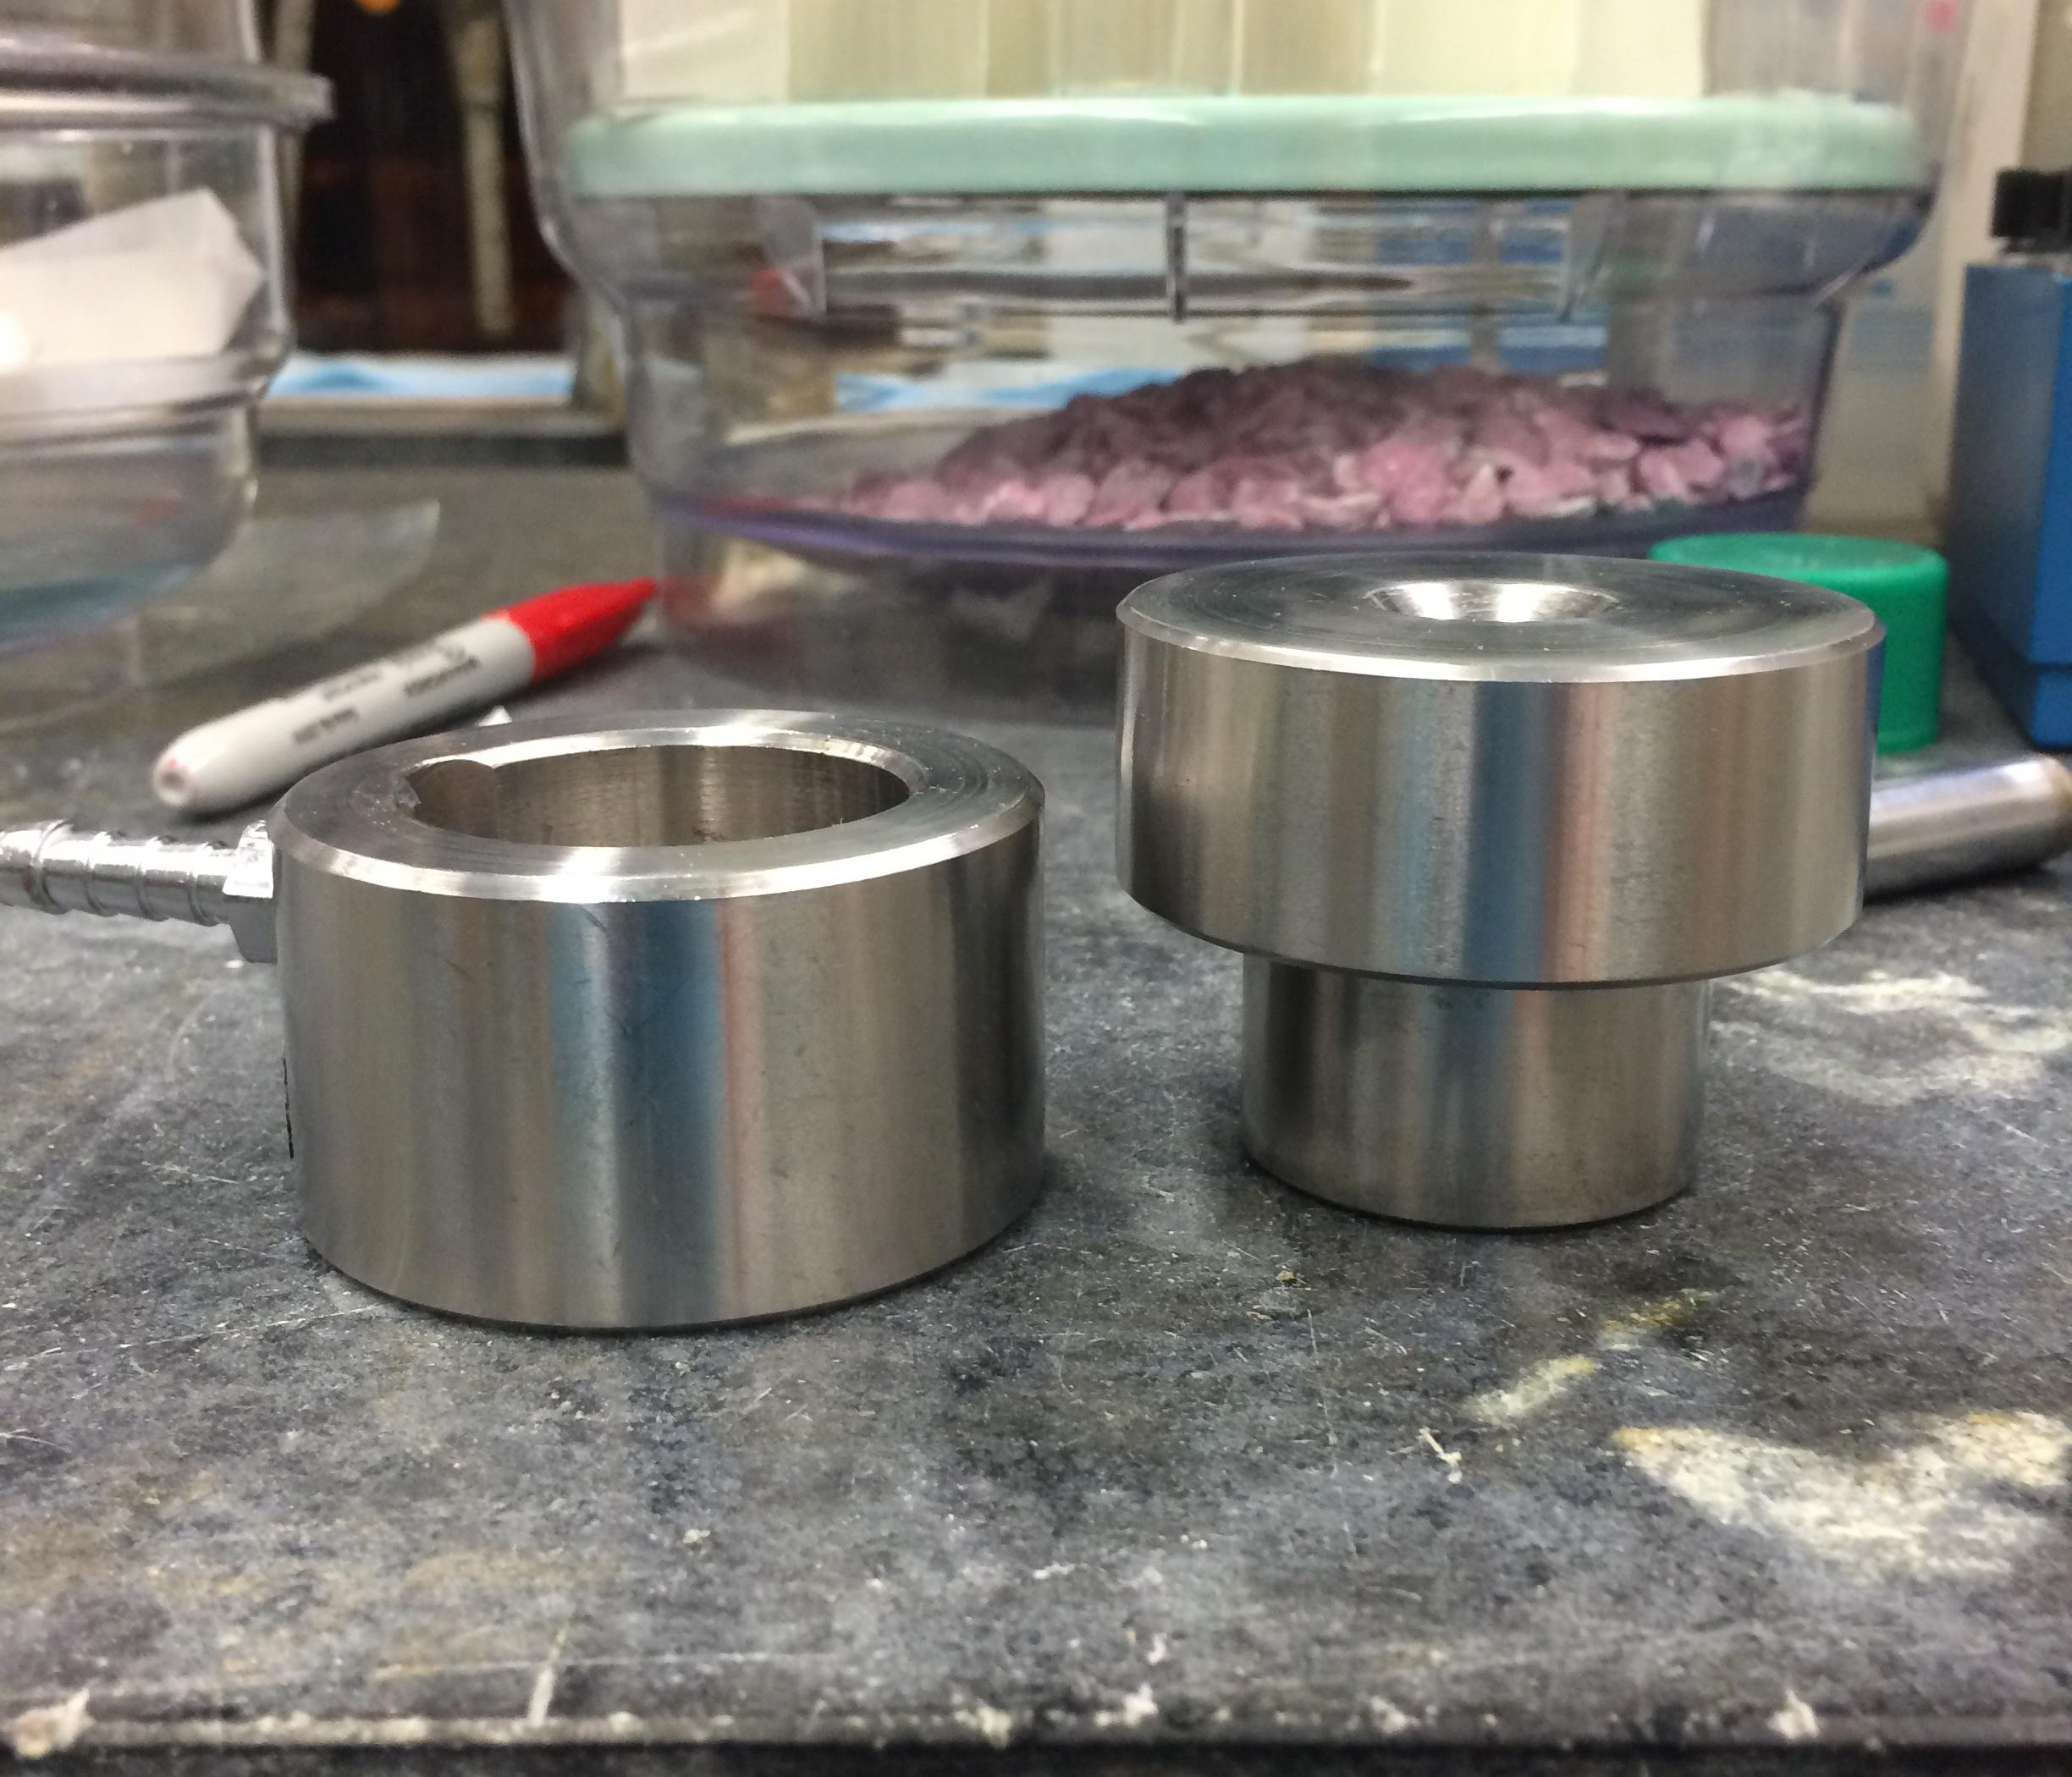
\includegraphics[scale=0.12]{images/die_opened.jpg}
		\caption{The two halves of the KBr die separated.}
		\label{fig:die_opened}
	\end{subfigure}%
	\begin{subfigure}{.5\textwidth}
		\centering
		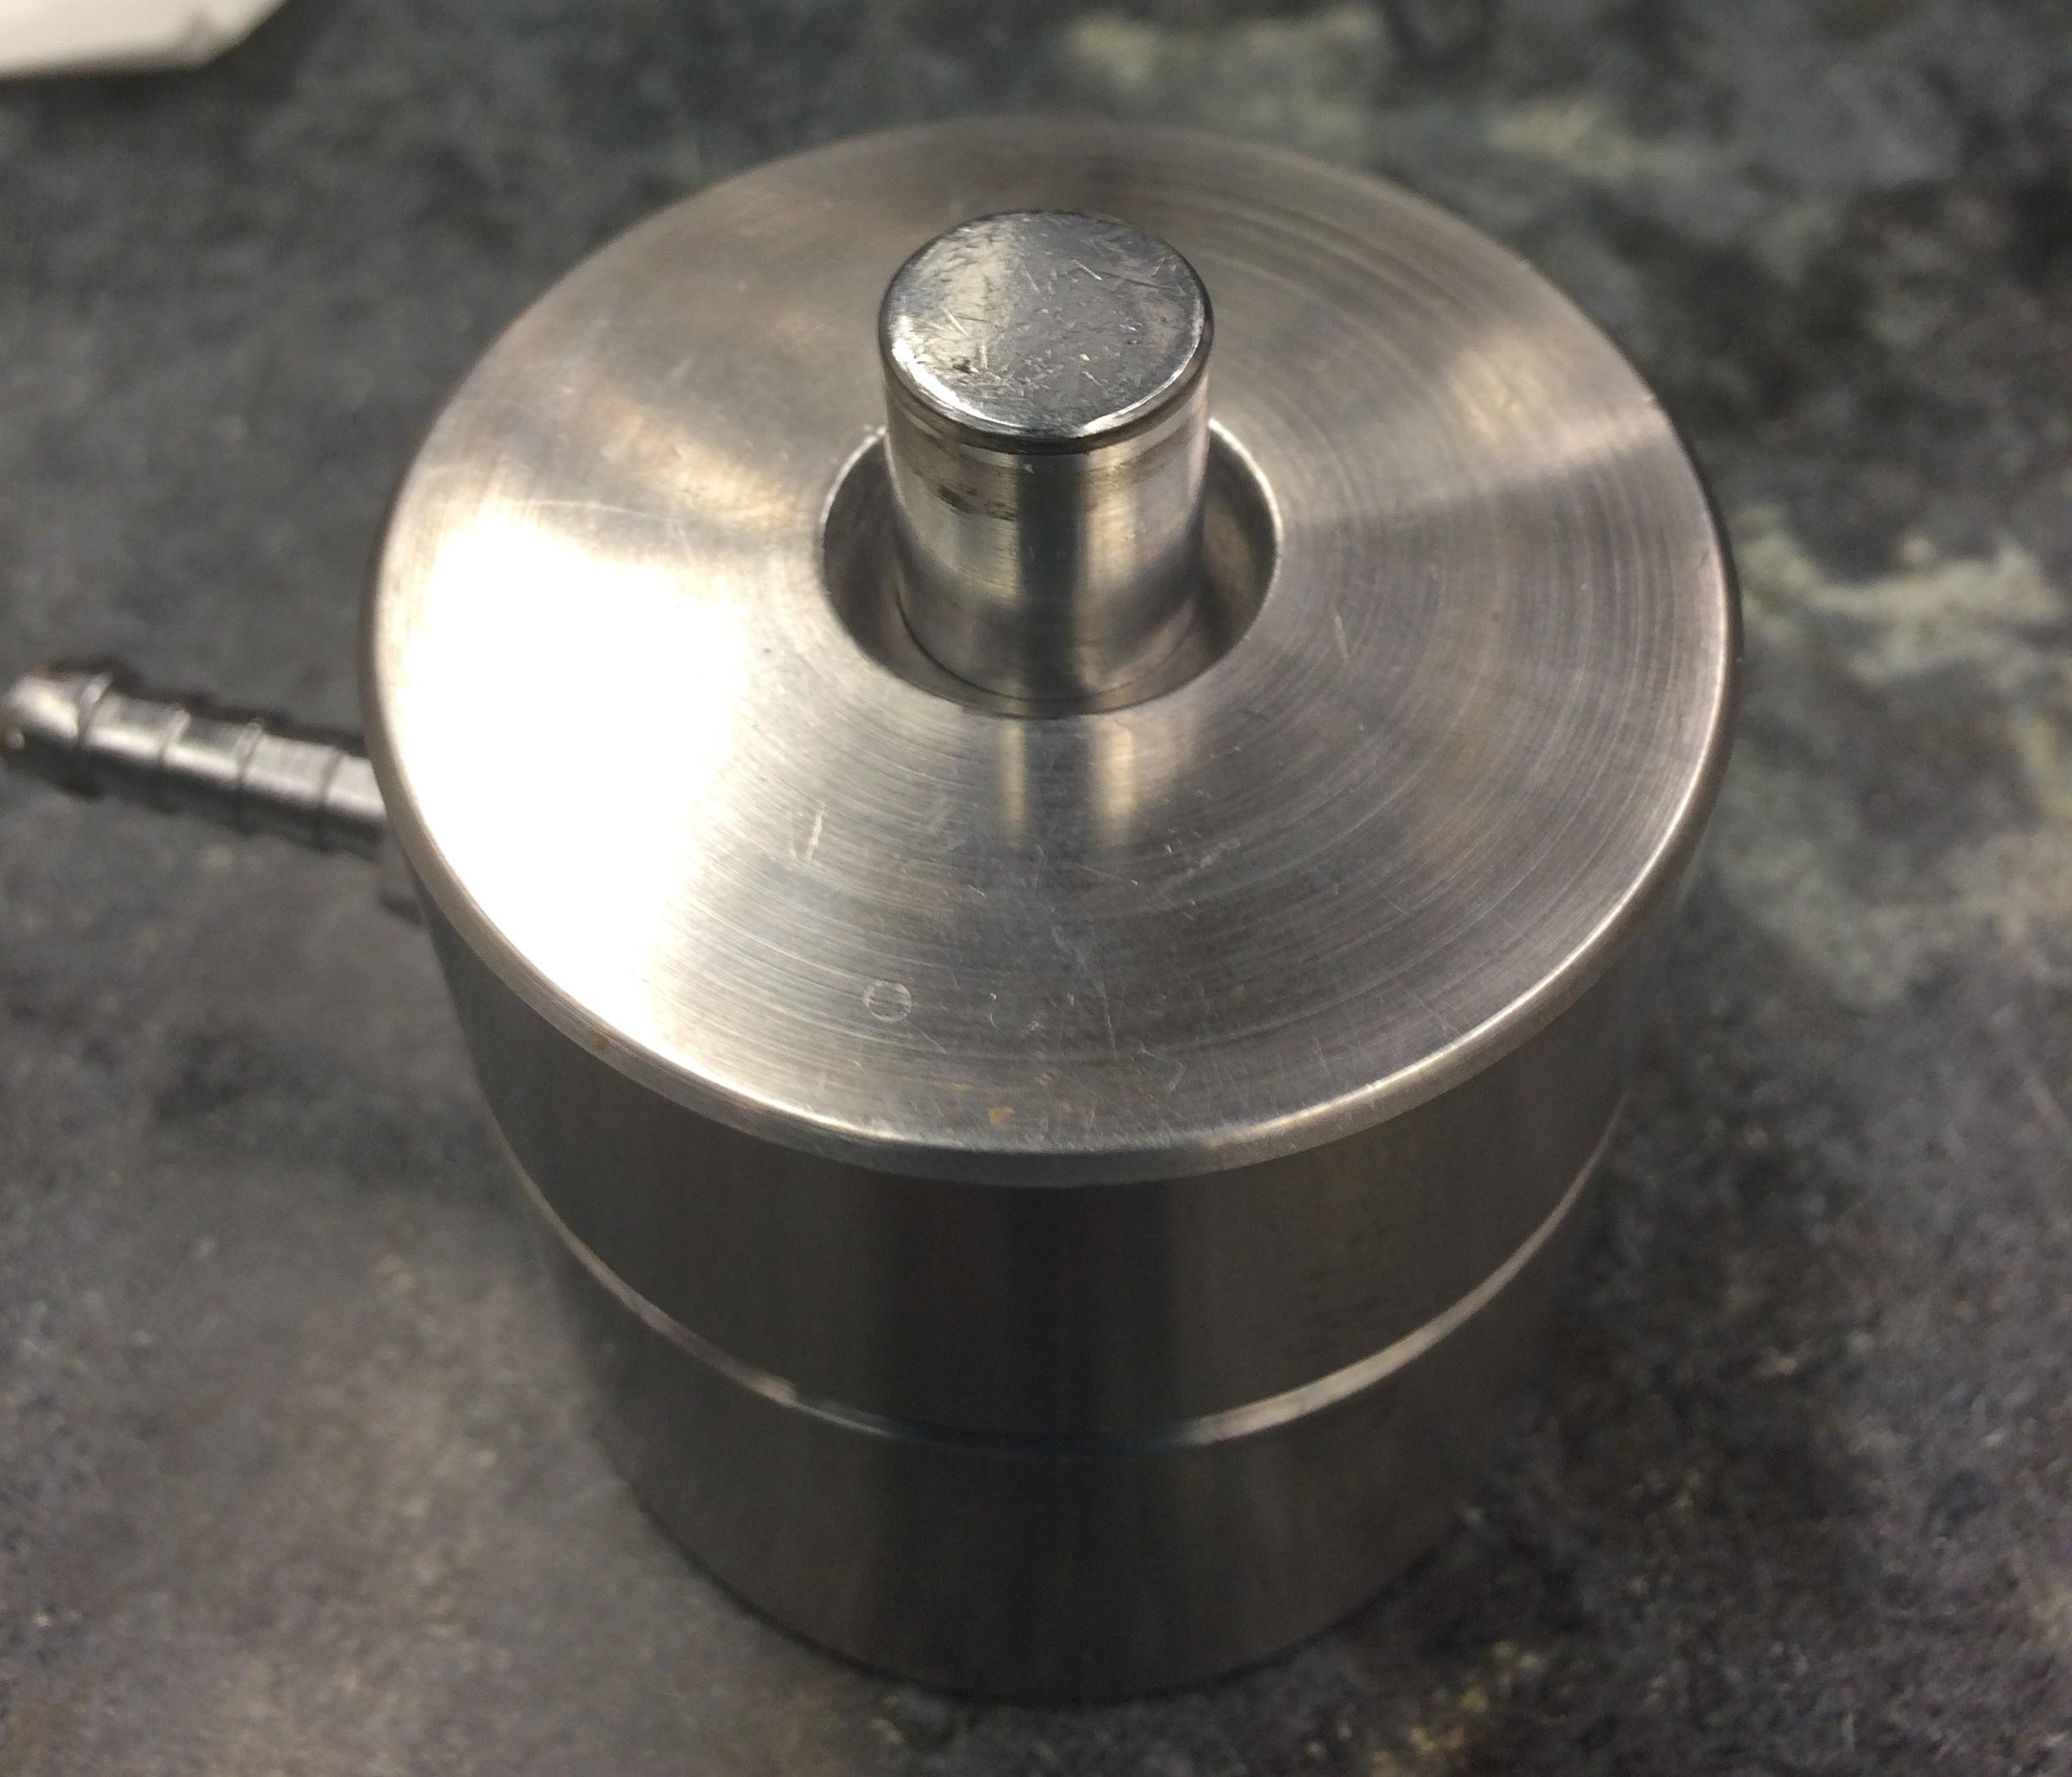
\includegraphics[scale=0.12]{images/die_closed.jpg}
		\caption{Assembled KBr die ready to be compressed.}
		\label{fig:die_closed}
	\end{subfigure}
	\caption{The KBr die used to compress clay powder into pellets.}
	\label{fig:KBr_die}
\end{figure}


Clay which has been pressed into a small thin disk however can be easier to work with in many lab settings, therefore if proper hydration of such samples is possible, they would be of great use in experiments. Such clay disks were prepared for this experiment by placing approximately 0.12$g$ to 0.13$g$ of clay powder into a KBr pellet die. The die used to form the pellets is displayed in Figure~\ref{fig:KBr_die}. A hydraulic press was used to compress the die to a force of approximately 12 tons. A small, sturdy clay pellet or disk was formed with a thickness of approximately 0.5$mm$ and a diameter of 1$cm$. While formed with a KBr die, no KBr was mixed with the clay powder. These samples were then placed in desiccators filled with saturated salt solutions for varying periods of time, until they were removed for XRD measurements. Samples of both types were usually left in desiccators for periods of one to five days before XRD measurements were conducted.

\subsubsection{XRD Measurments}
The $d_{001}$ basal spacing of the samples was measured using a a Bruker D8-Discover X-Ray Diffractometer. Standard locked coupled scans varied the $2\theta$ axis, measuring the reflections at each angle.

Hydrated clay powder was placed into elongated depressions on square glass plates. A second glass plate was then used to press the clay into the depression. After the second plate was removed, large particles of clay on the edge of the depression were wiped away, and the plate was mounted into the diffractometer. A Z scan was first performed to ensure that the X-ray beam was incident in the middle portion of the depression, approximately half way down. Locked coupled scans were performed over the  $2\theta$ angles from $2^\circ$ to $10^\circ$ for all samples.

Hydrated clay pellets underwent a similar process. Pellets were attached to a flat glass plate using a small piece of double sided tape. This plate was then placed in the diffractometer, using 2$mm$ spacer bars to recess the entire plate in the sample mount, to account for the pellet protruding from the surface. A beam height limiter had to be used with the pellets as their diameter was somewhat shorter than most other samples used in the device. A Z scan was again used to center the bean in the center of the disk, between its two faces. A rocking curved scan positioned the $\theta$ axis to the location of maximum intensity, compensating for the fact that the disks do not lie perfectly flat on the plate. Locked coupled scans across the $2\theta$ angle from $2^\circ$ to $10^\circ$ were also performed.

\subsection{Results and Discussion}
\subsubsection{Clay Pellets}

\begin{figure}
	\centering
	\begin{subfigure}{.5\textwidth}
		\centering
		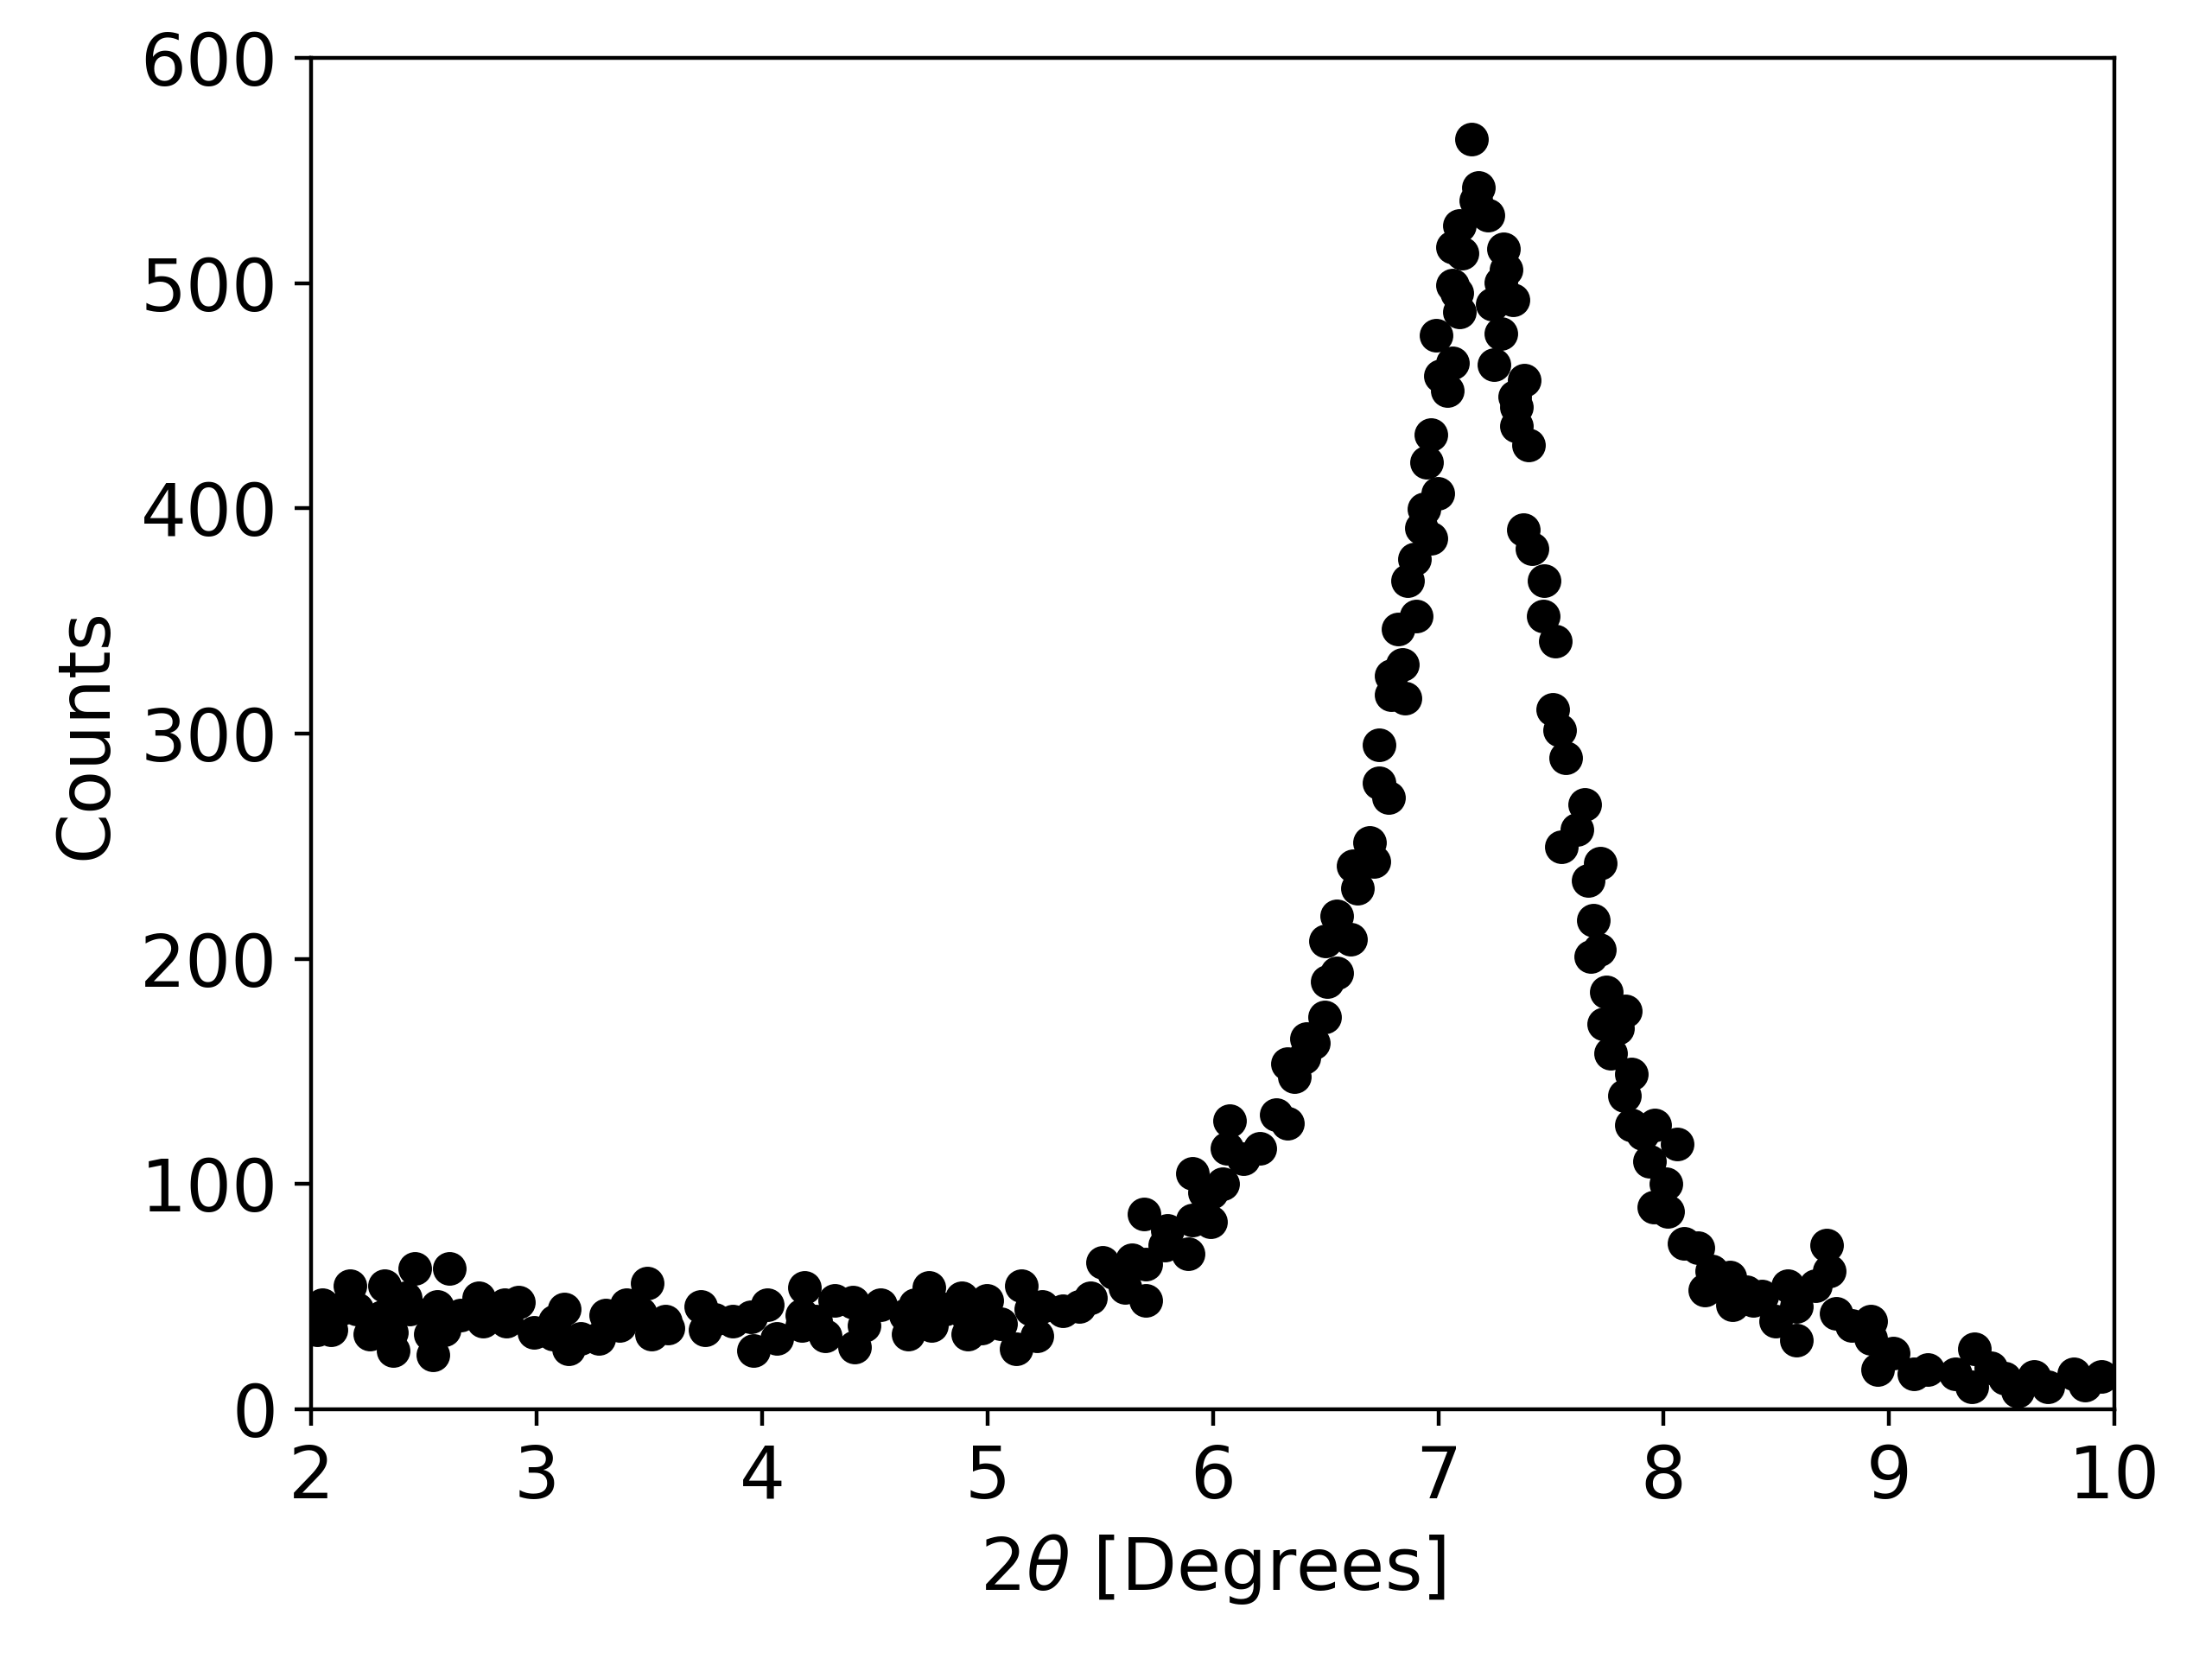
\includegraphics[scale=0.5]{images/80_1d.png}
		\caption{Left for 20 hours, peak at $2\theta=7.1^\circ$ corresponding to $d_{001}=12.4\angstrom$.}
		\label{fig:80_1d}
	\end{subfigure}%
	\begin{subfigure}{.5\textwidth}
		\centering
		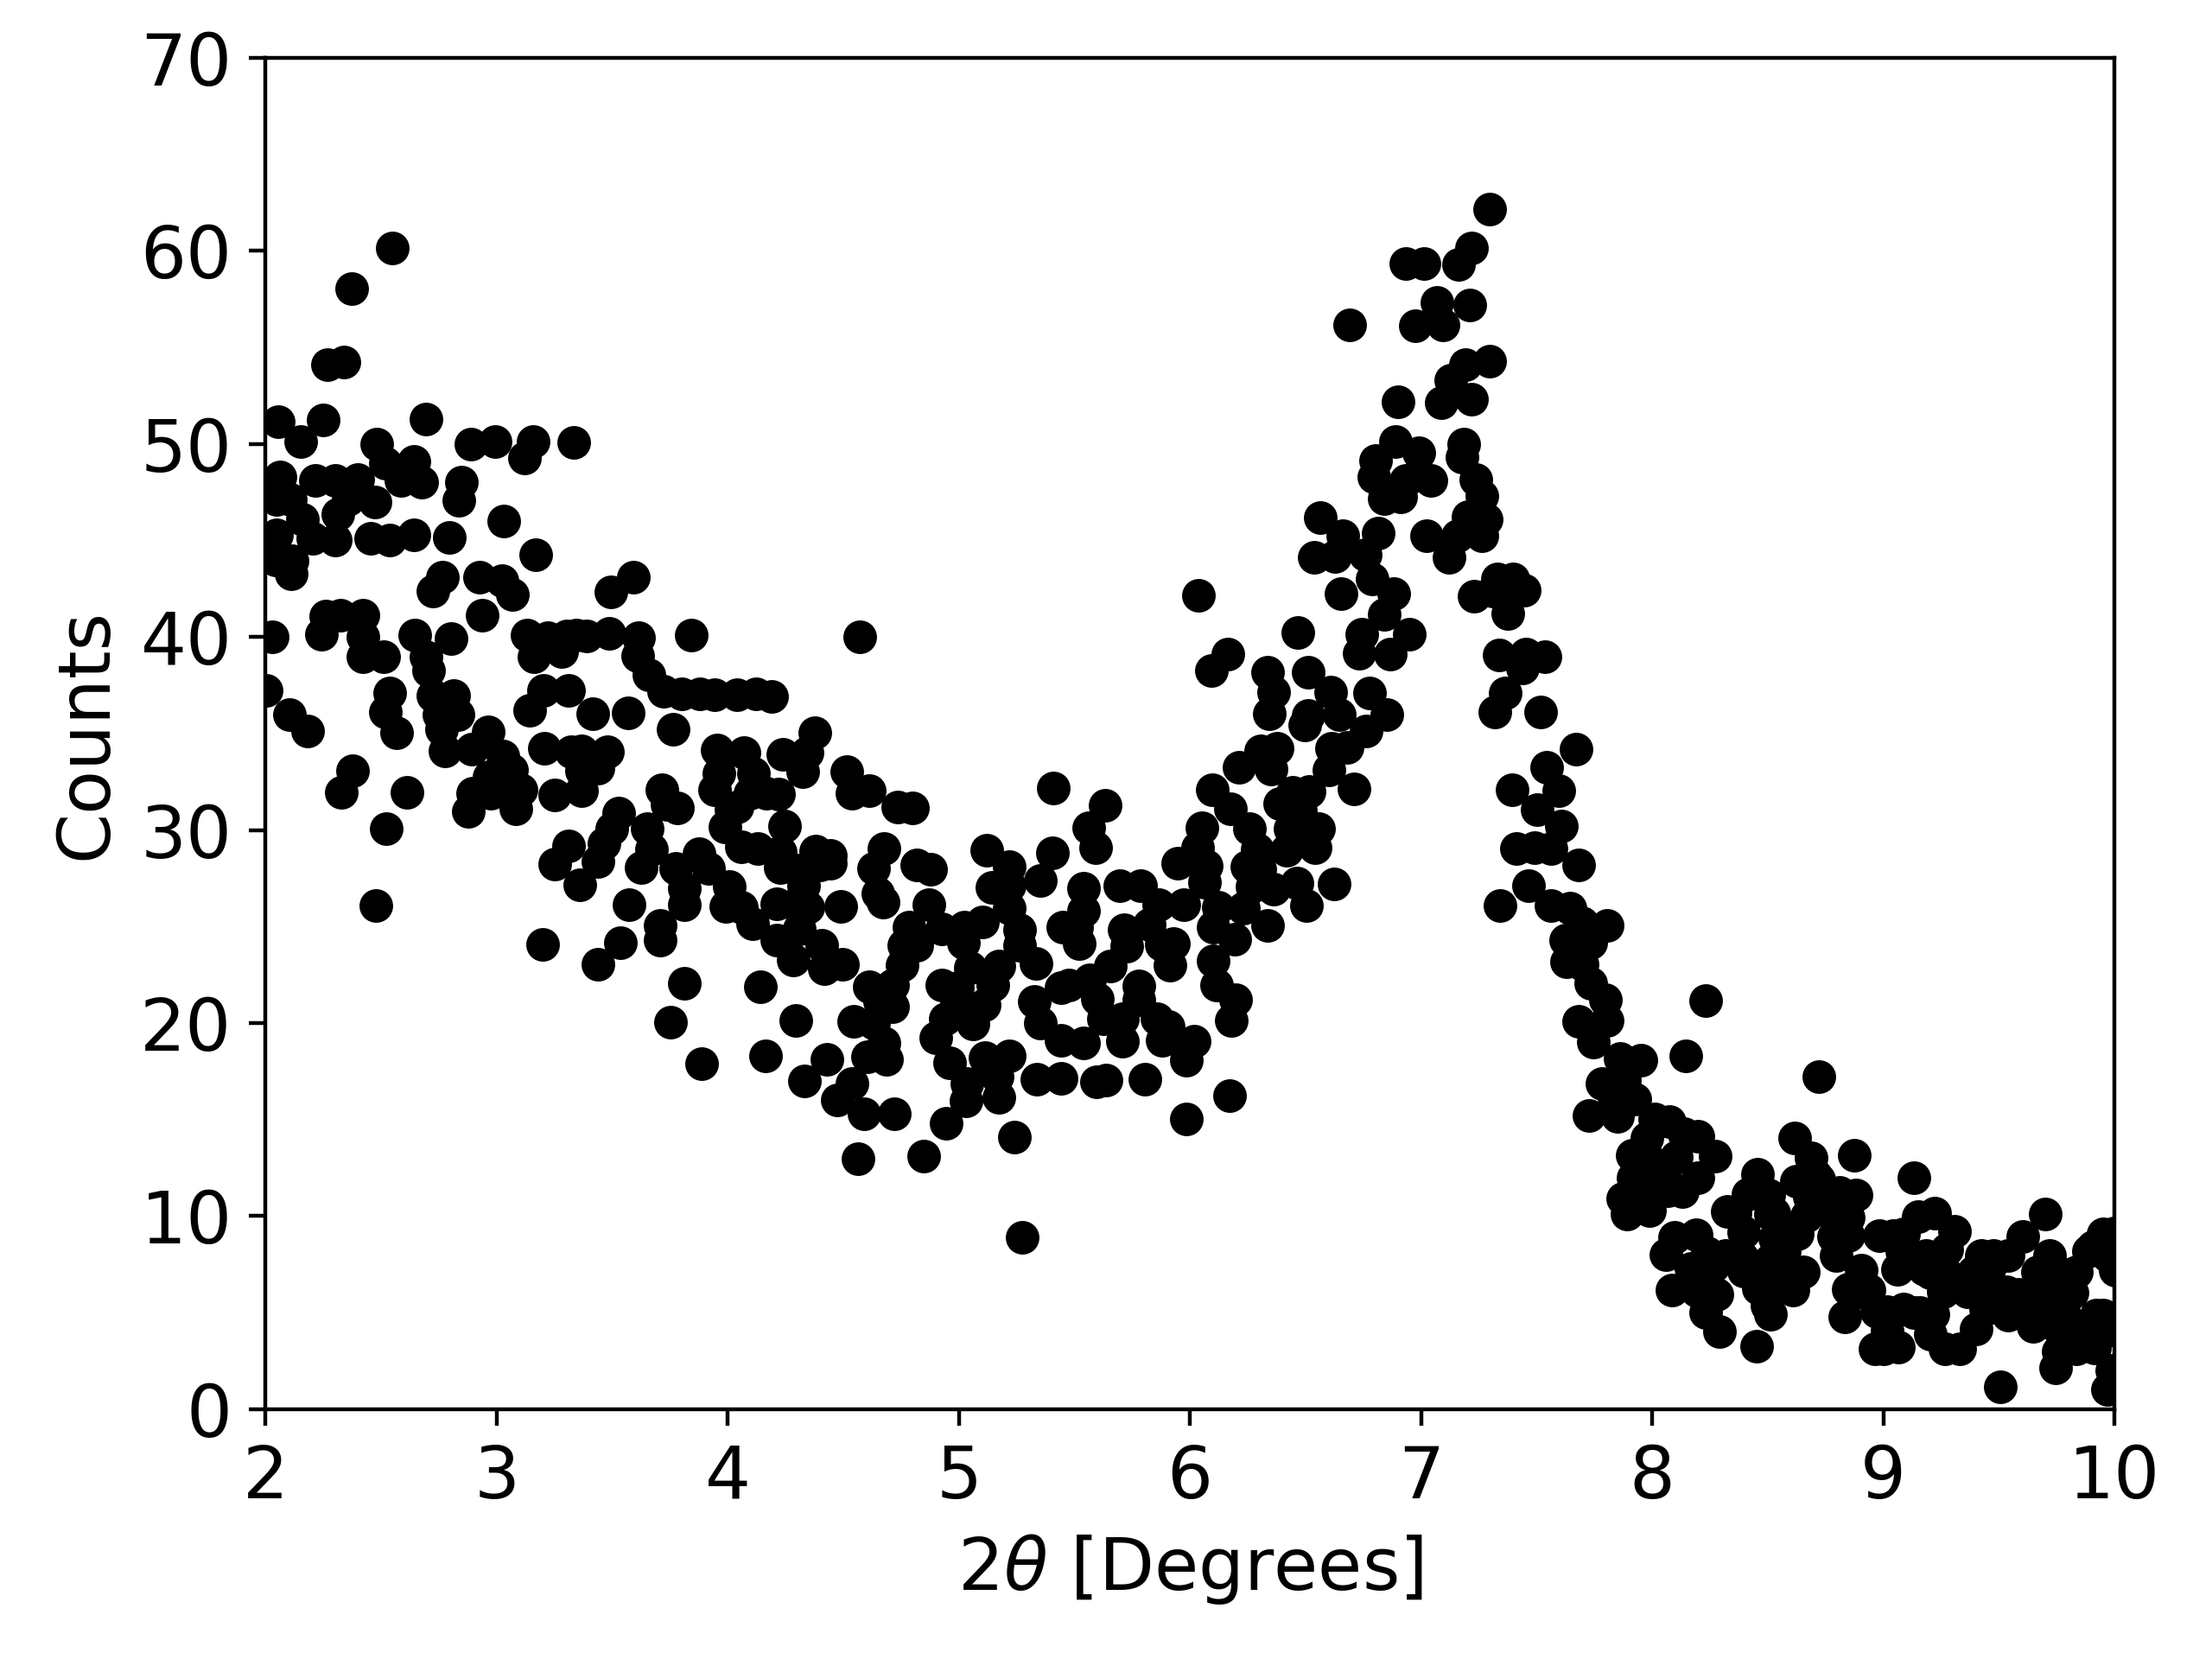
\includegraphics[scale=0.5]{images/80_3d.png}
		\caption{Left for 70 hours, peak at $2\theta=7.3^\circ$ corresponding to $d_{001}=12.1\angstrom$.}
		\label{fig:80_3d}
	\end{subfigure}
	\caption{XRD Bragg peaks of clay pellets left in 80\% humidity.}
	\label{fig:80_pellet}
\end{figure}

The XRD peaks of samples left in desiccators for approximately one and three days are presented in Figure~\ref{fig:80_pellet}. Both peaks indicate that the basal spacing is only $d_{001}\approx 12\angstrom$, indicating that there is only a monolayer of water present in the montmorillonite. The full width half maximum (FWHM) of the peak in Figure~\ref{fig:80_1d} is less than $1^\circ$, indicating that the monolayer is quite homogeneous, and that there are very few, if any locations where there is the formation of a bilayer in the sample. It is more difficult to determine the breadth of the peak in Figure~\ref{fig:80_3d}, but due to the smaller basal spacing in accordance with the center of the peak location, it is also very likely that there is but a monolayer of water present between the clay sheets.

\begin{figure}
	\centering
	\begin{subfigure}{.5\textwidth}
		\centering
		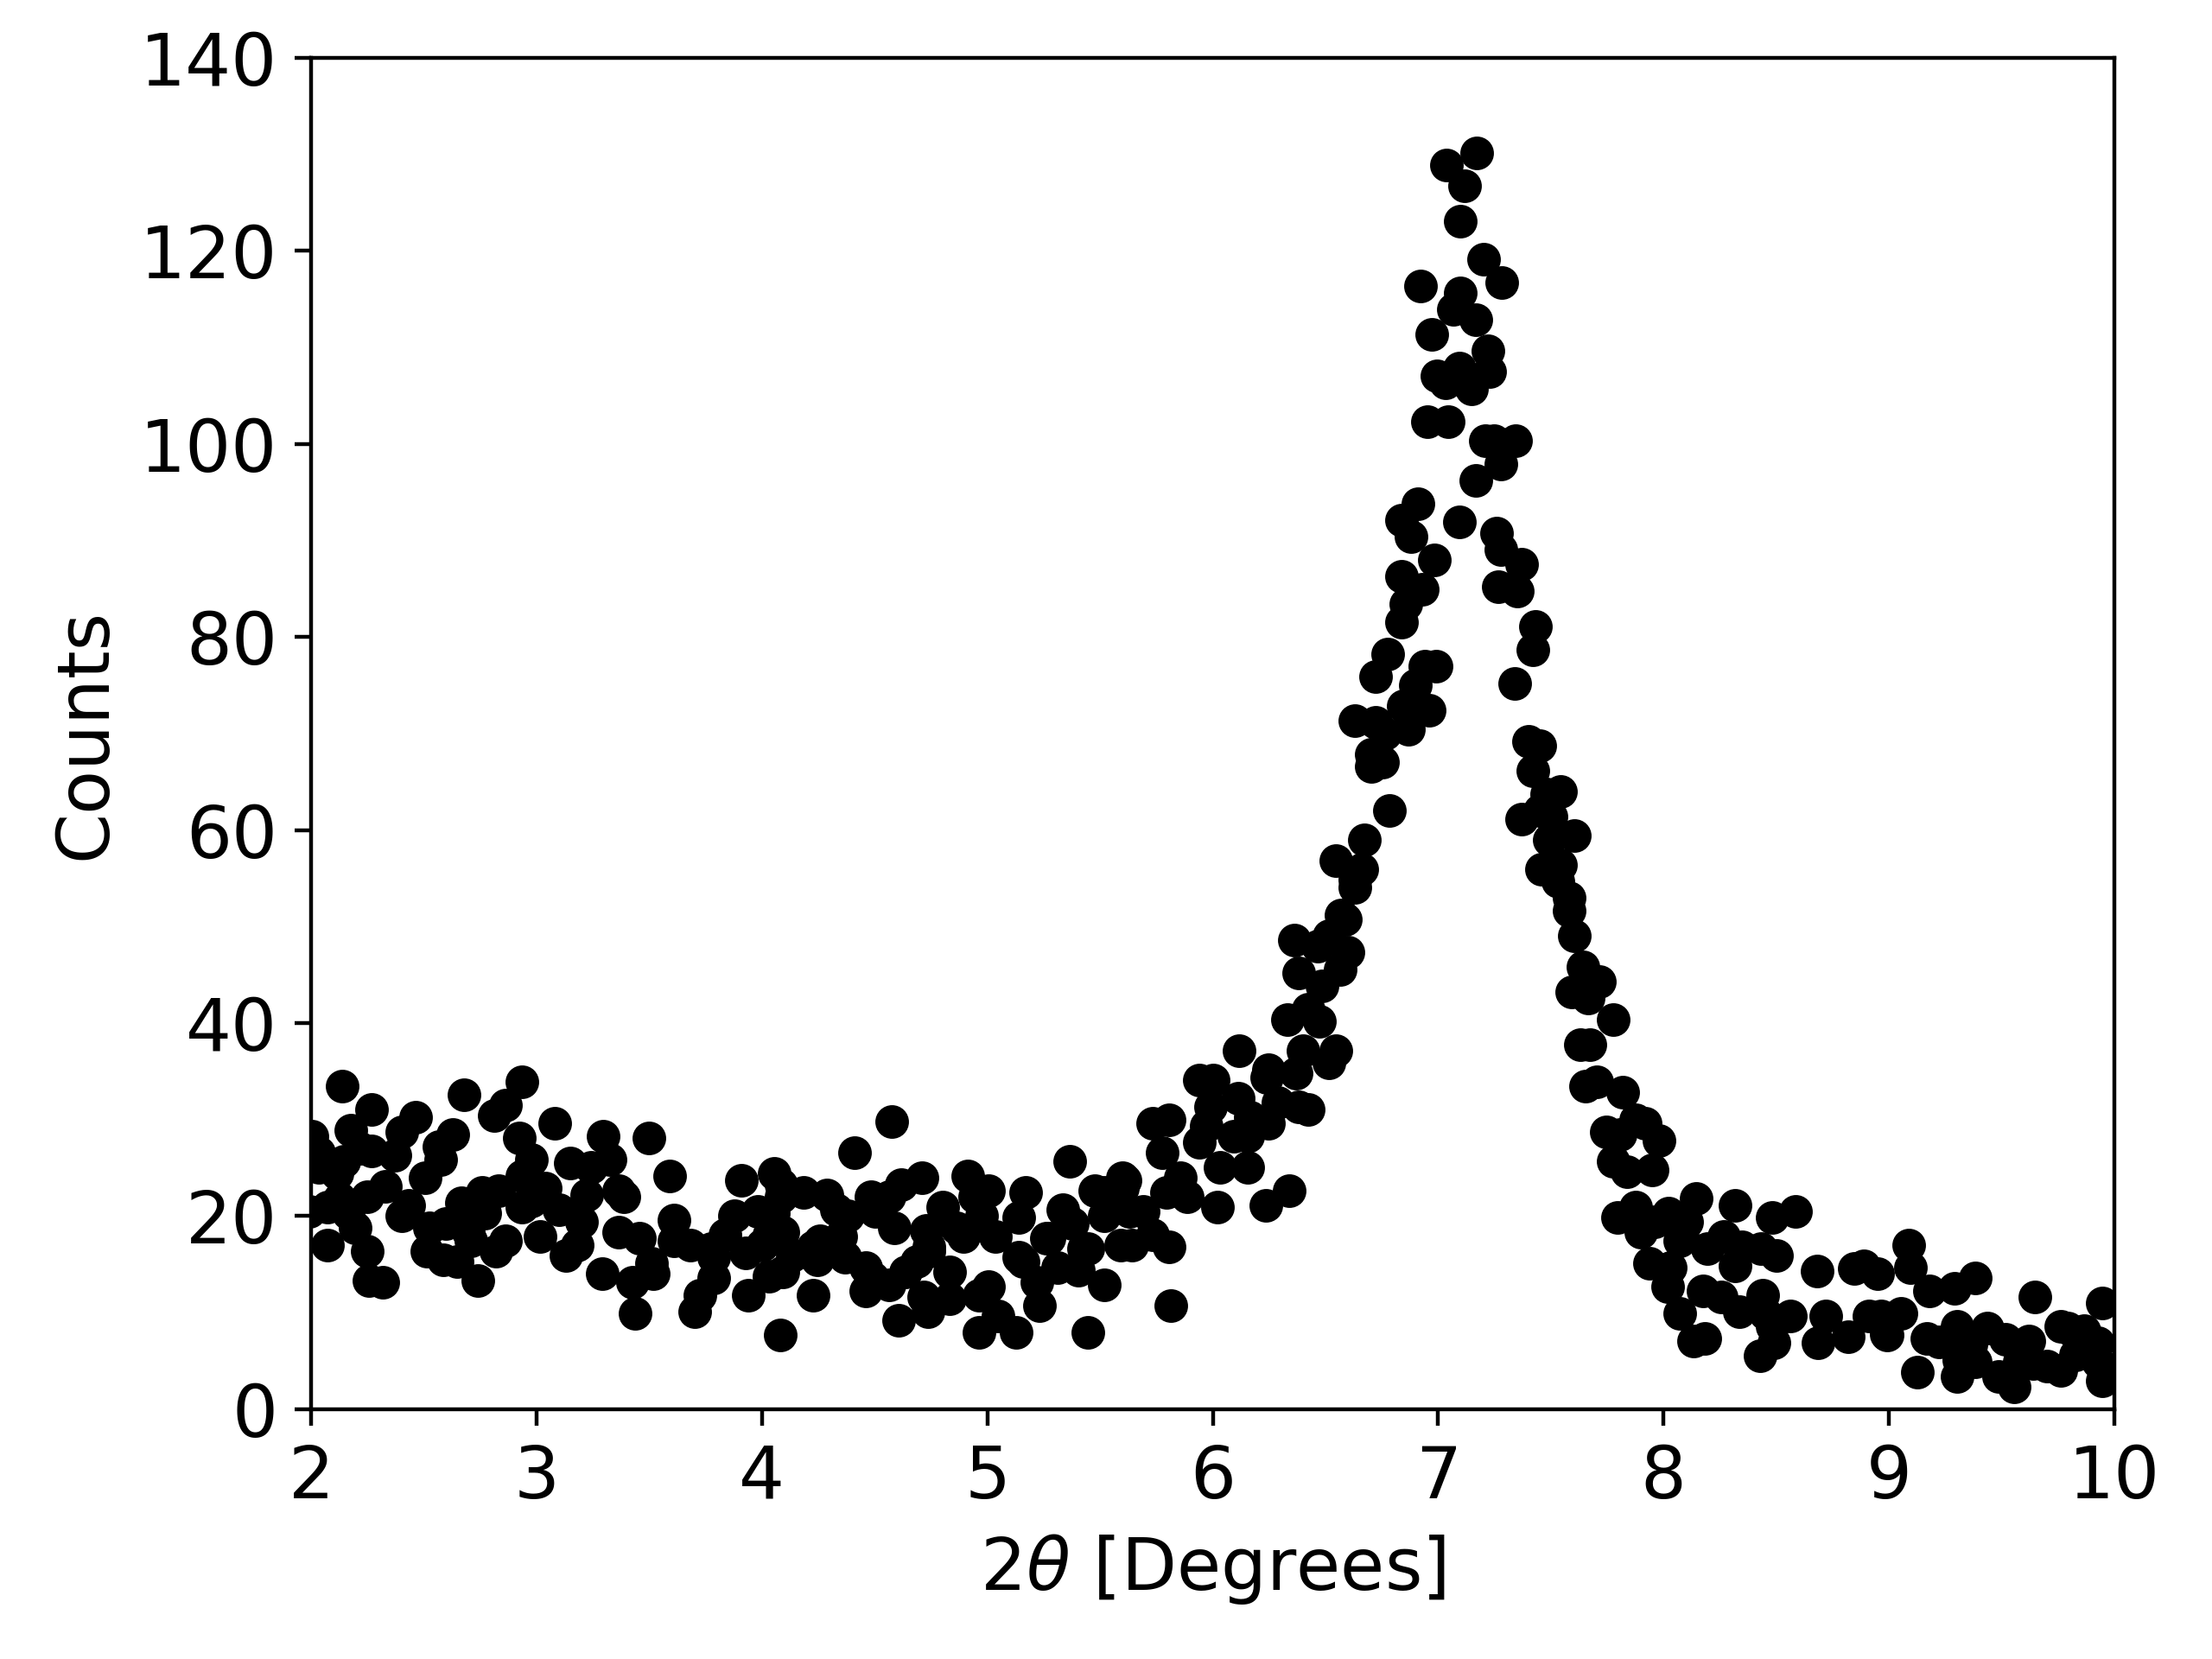
\includegraphics[scale=0.5]{images/97_plt_1d.png}
		\caption{Left for 20 hours, peak at $2\theta=7.2^\circ$ corresponding to $d_{001}=12.3\angstrom$.}
		\label{fig:97_plt_1d}
	\end{subfigure}%
	\begin{subfigure}{.5\textwidth}
		\centering
		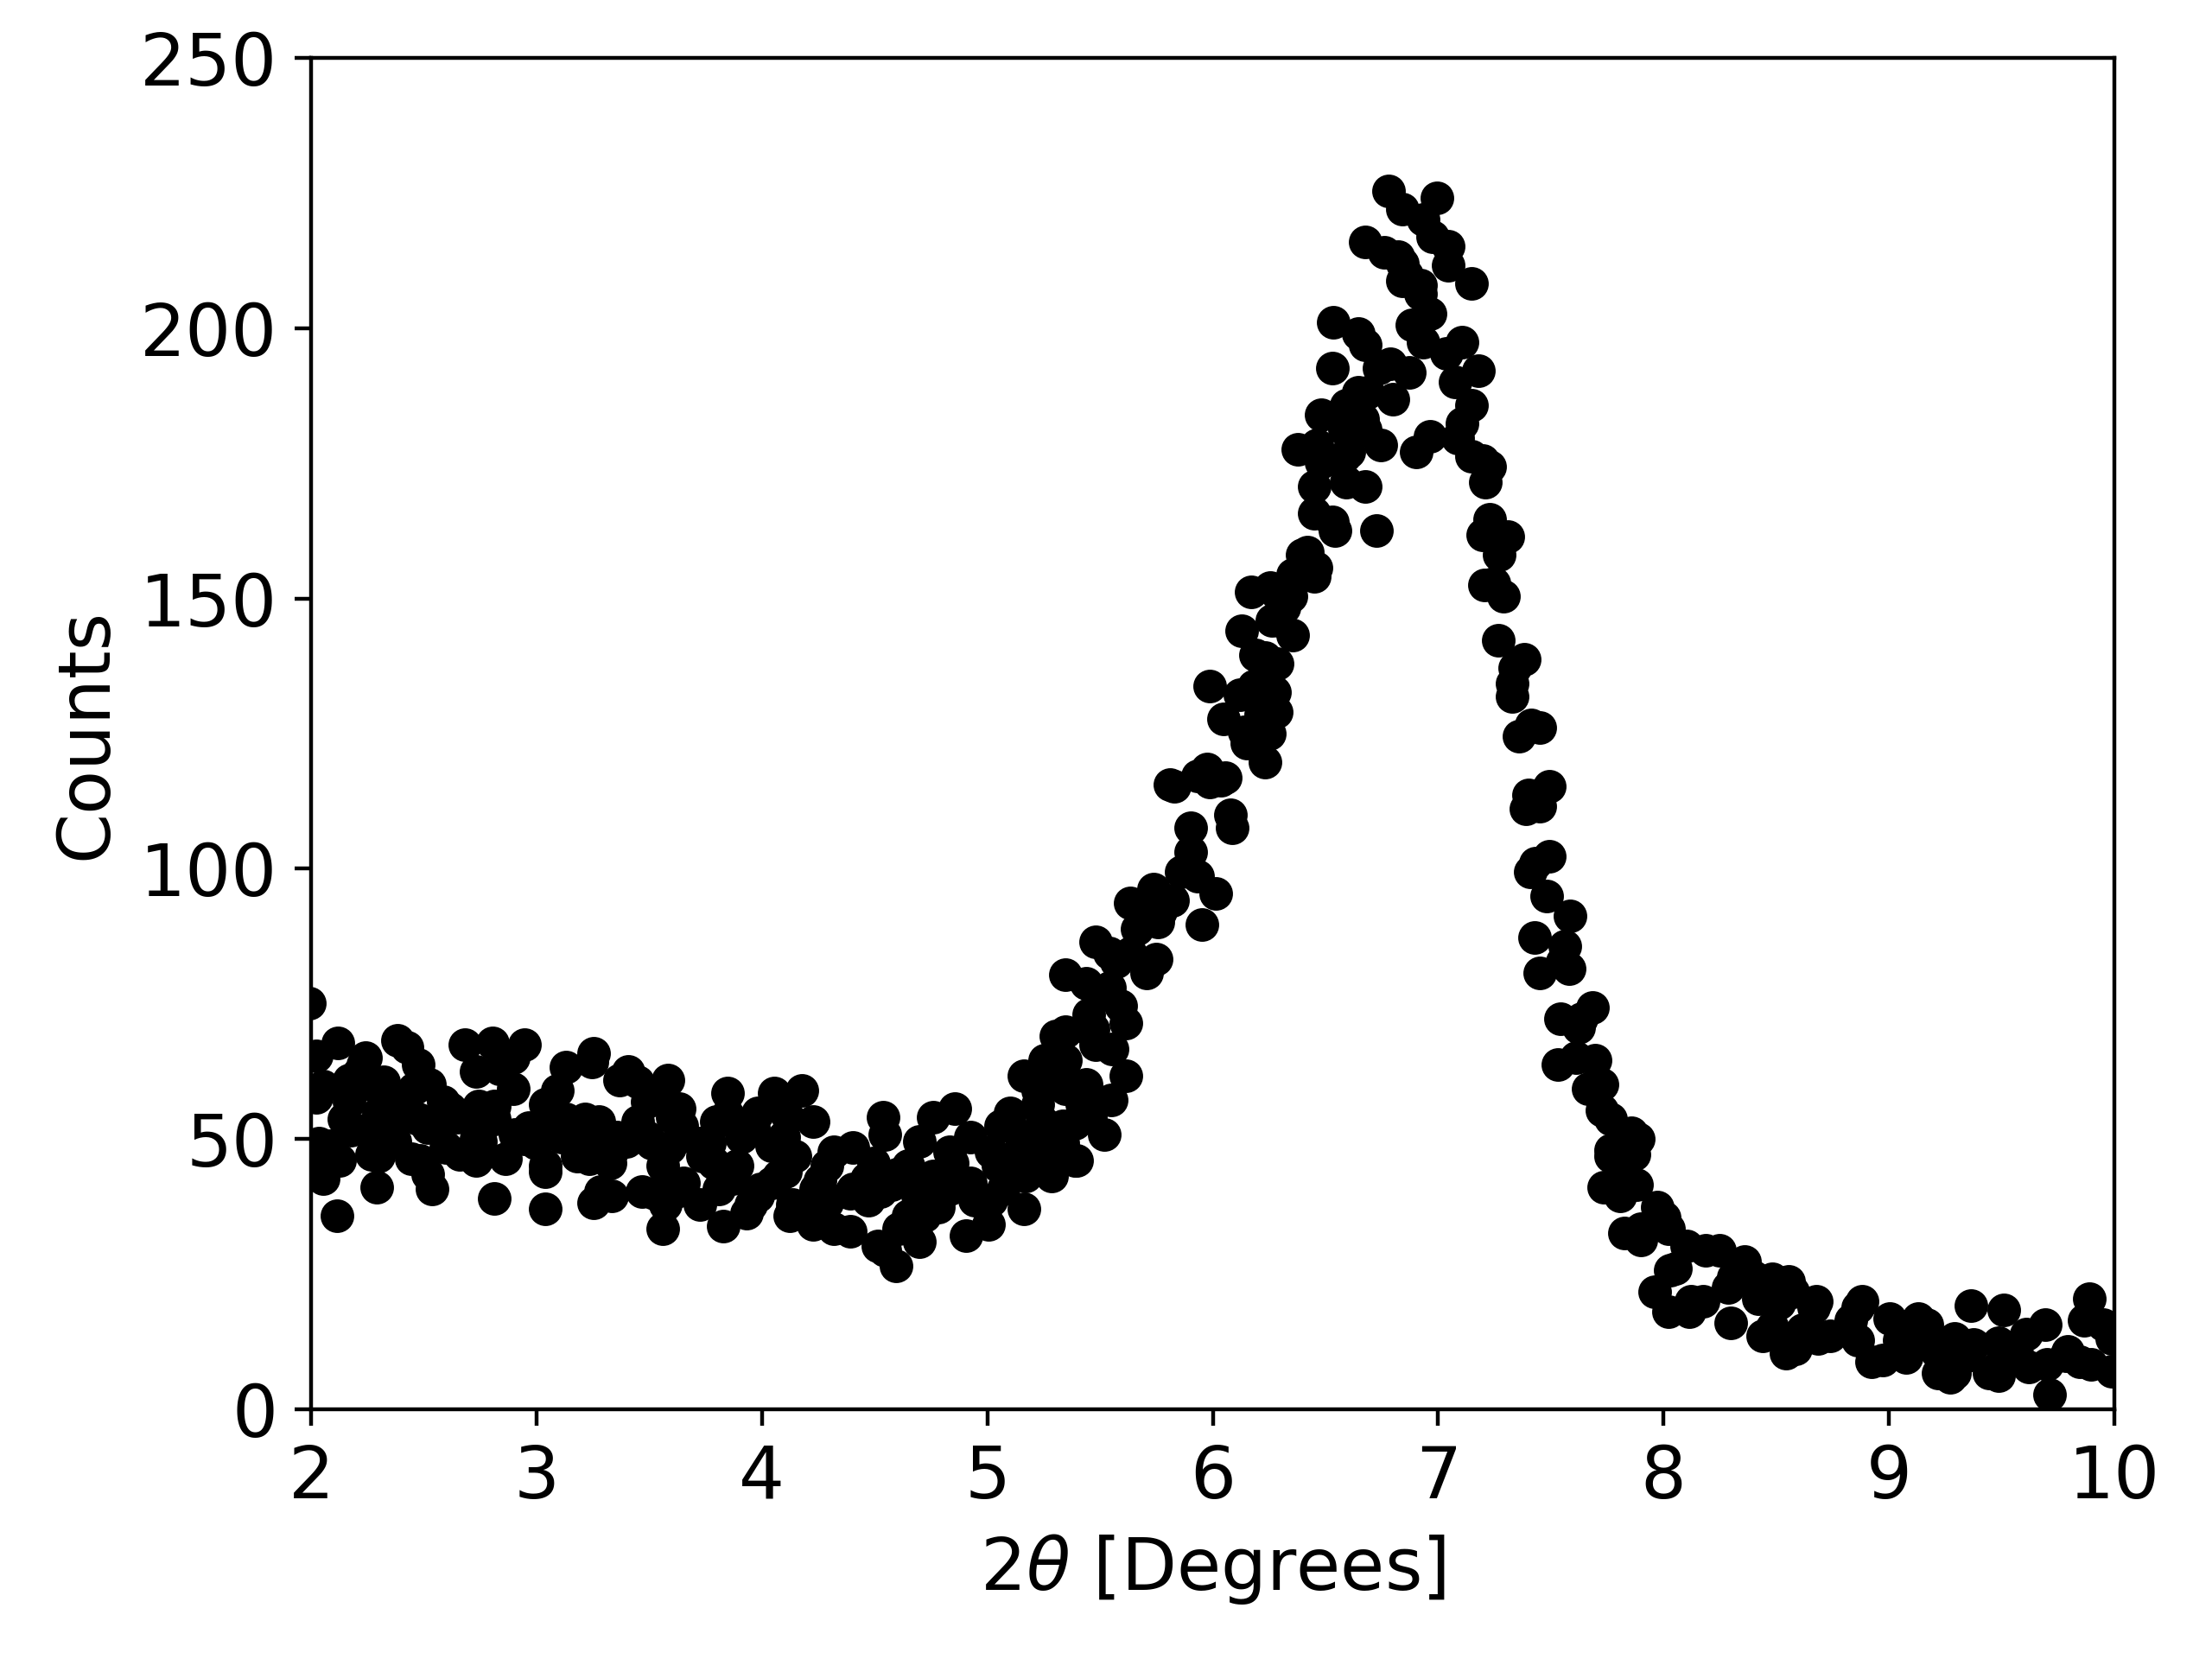
\includegraphics[scale=0.5]{images/97_plt_3d.png}
		\caption{Left for 70 hours, peak at $2\theta=7.0^\circ$ corresponding to $d_{001}=12.7\angstrom$.}
		\label{fig:97_plt_3d}
	\end{subfigure}
	\caption{XRD Bragg peaks of clay pellets left in 97\% humidity.}
	\label{fig:97_pellet}
\end{figure}

Moving up in humidity to the $K_2SO_4$ desiccator, which should have maintained a relative humidity of $p/p_0=0.97$, a similar result is observed. After one day, as shown in Figure~\ref{fig:97_plt_1d}, the sample only has a monolayer of water which is very homogeneous. Increasing the time it is left in the desiccator to three days does have a slight effect. As seen in Figure~\ref{fig:97_plt_3d}, the main peak is still at $7.3^\circ$, indicating a monolayer, but a small bump is now visible at approximately $5.5^\circ$, which corresponds to a bilayer of water. Although small, this does indicate a certain level of heterogeneity in the hydration.


\subsubsection{Clay Powder}

\begin{figure}
	\centering
	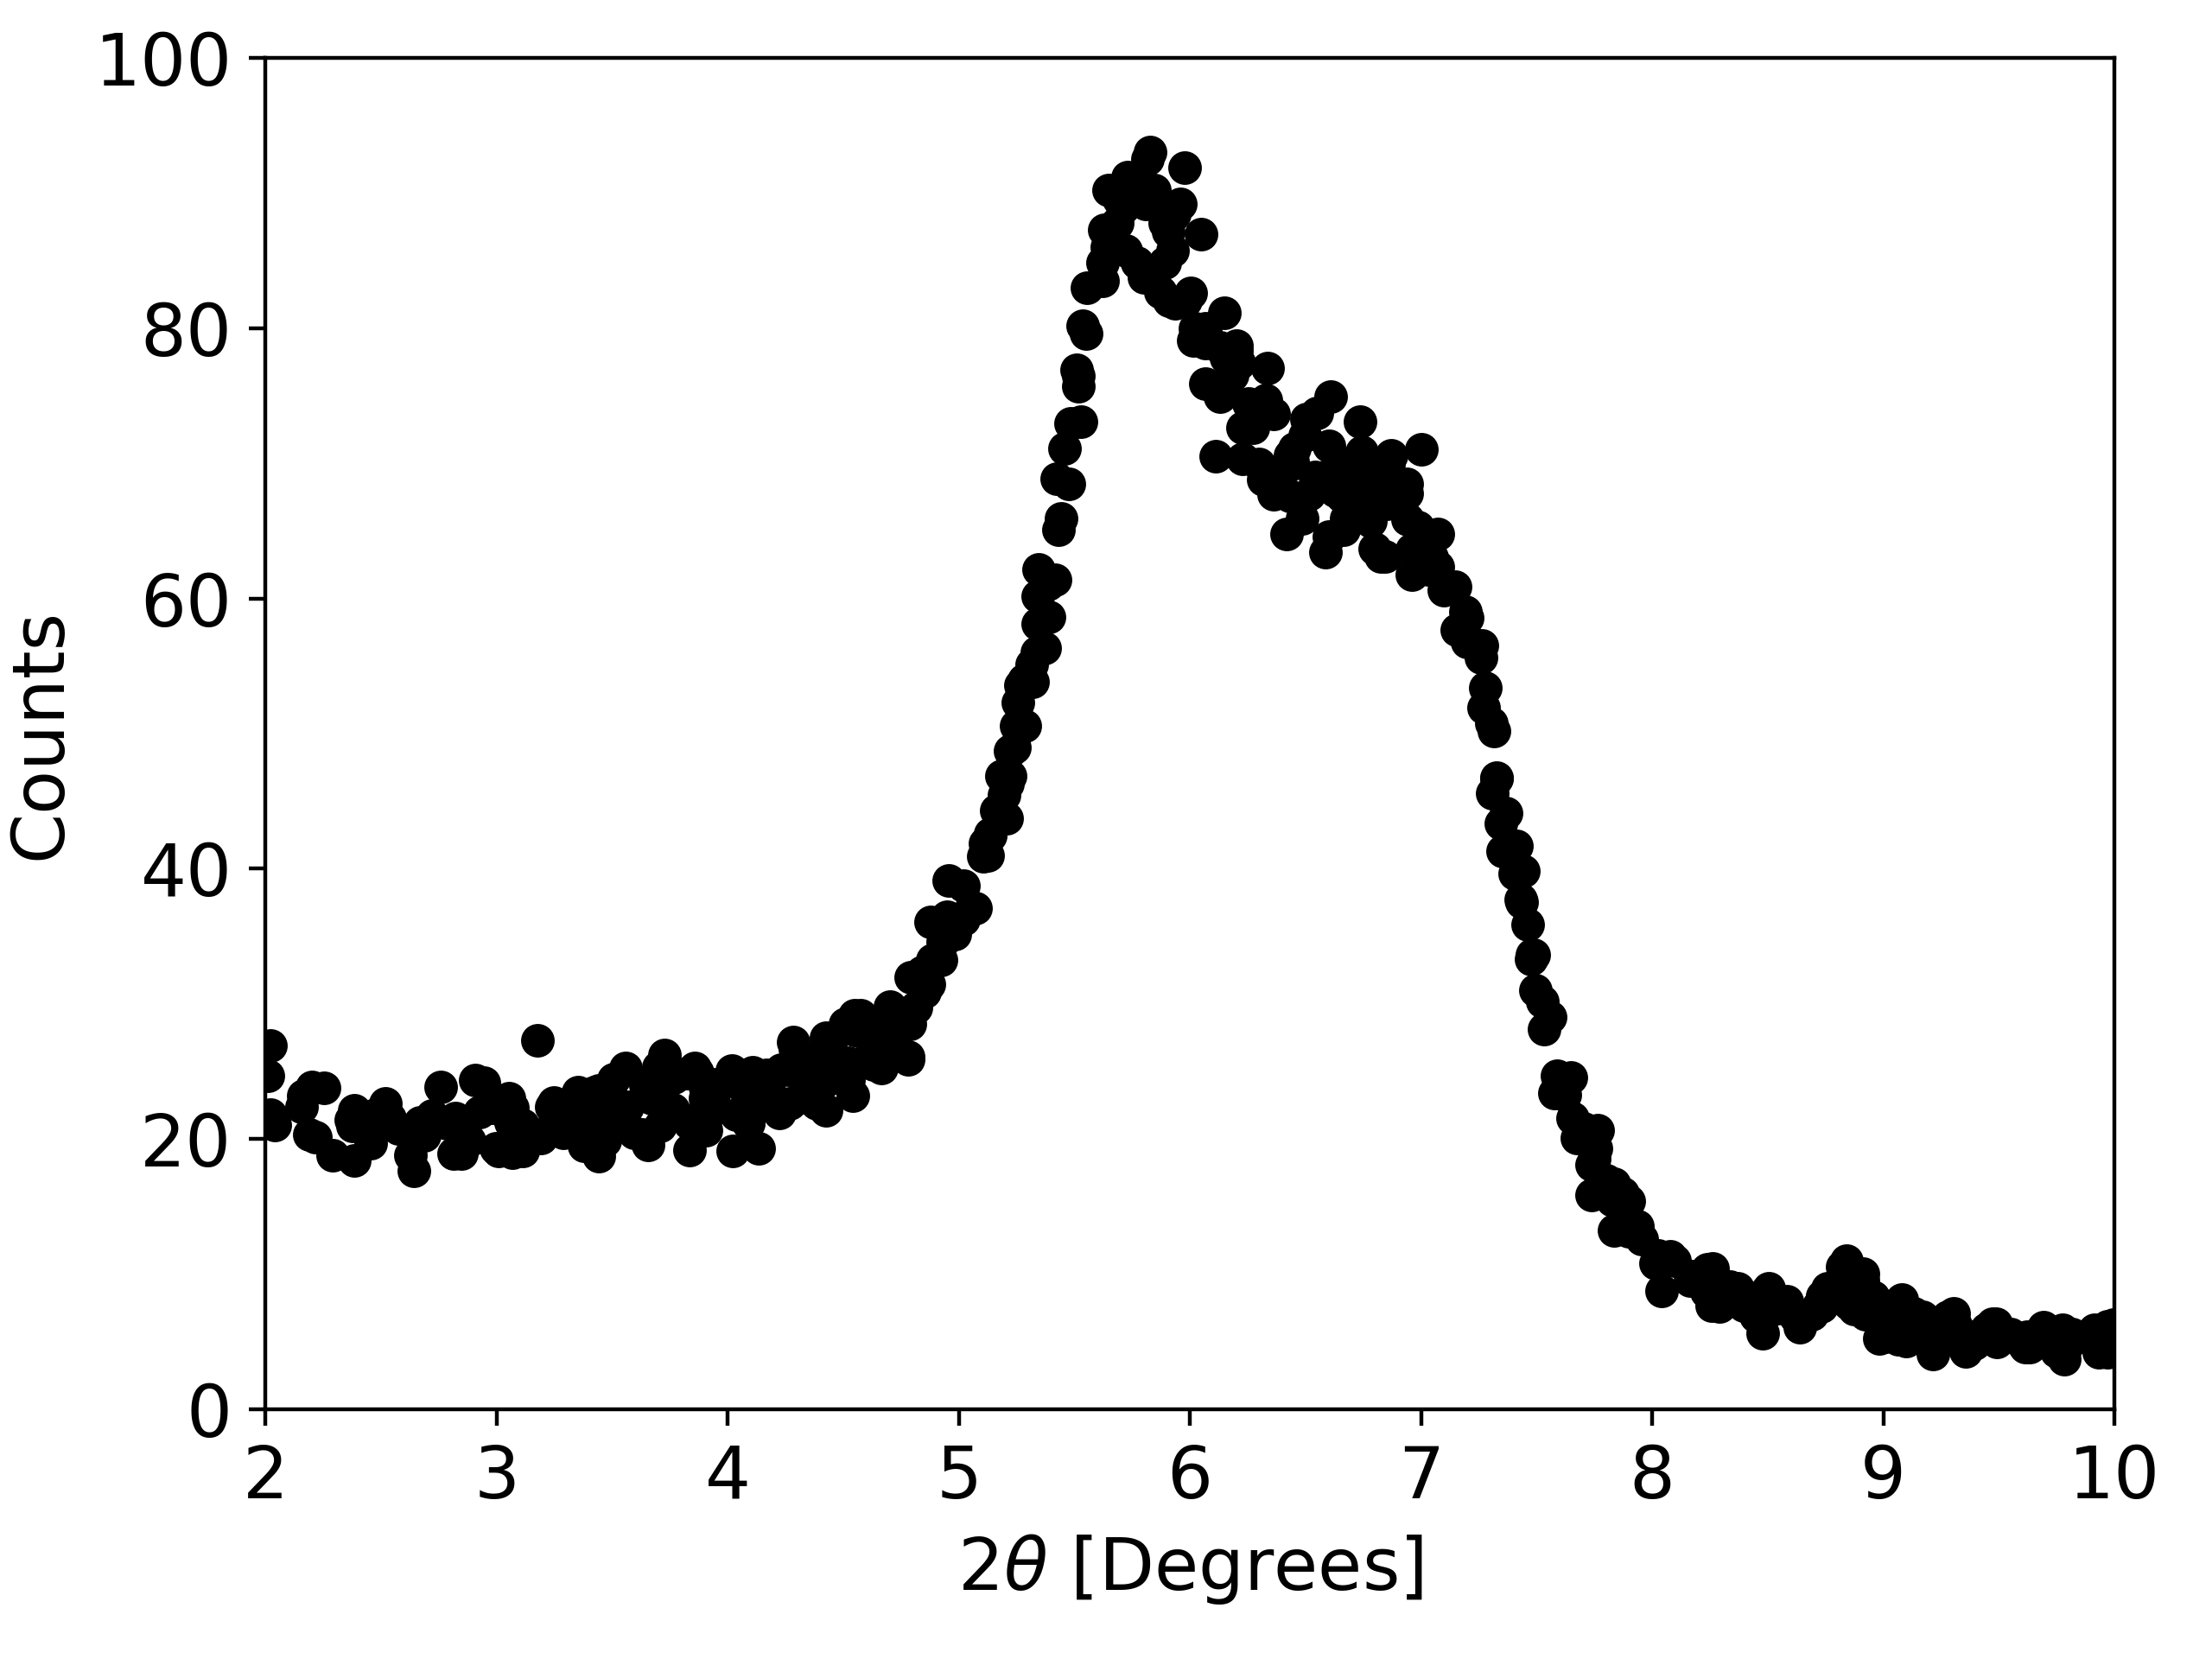
\includegraphics[scale=0.7]{images/97_pwd_3d.png}
	\caption{Peak of clay powder kept at 97\% humidity for three days, with $d_{001}=15.1\angstrom$, and a FWHM of $2.0^\circ$.}
	\label{fig:97_pwd_3d}
\end{figure}

Leaving clay powder samples at 97\% humidity for three days produces a very different result compared to the clay pellets which were exposed for a comparable amount of time. In Figure~\ref{fig:97_pwd_3d}, we see that the principal peak is now that corresponding to a $15.1\angstrom$ basal spacing, indicating a bilayer of water, and a second peak, of just a slightly lower magnitude, is observed at $2\theta=7^\circ$, corresponding to a monolayer of water. From this, it would appear that the powder samples are much more easily hydrated than the clay pellets, and that in this sample, there is mainly a bilayer of water between sheets of clay, though it is very heterogeneous, with a large portion of the clay also having a monolayer.

\begin{figure}
	\centering
	\begin{subfigure}{.5\textwidth}
		\centering
		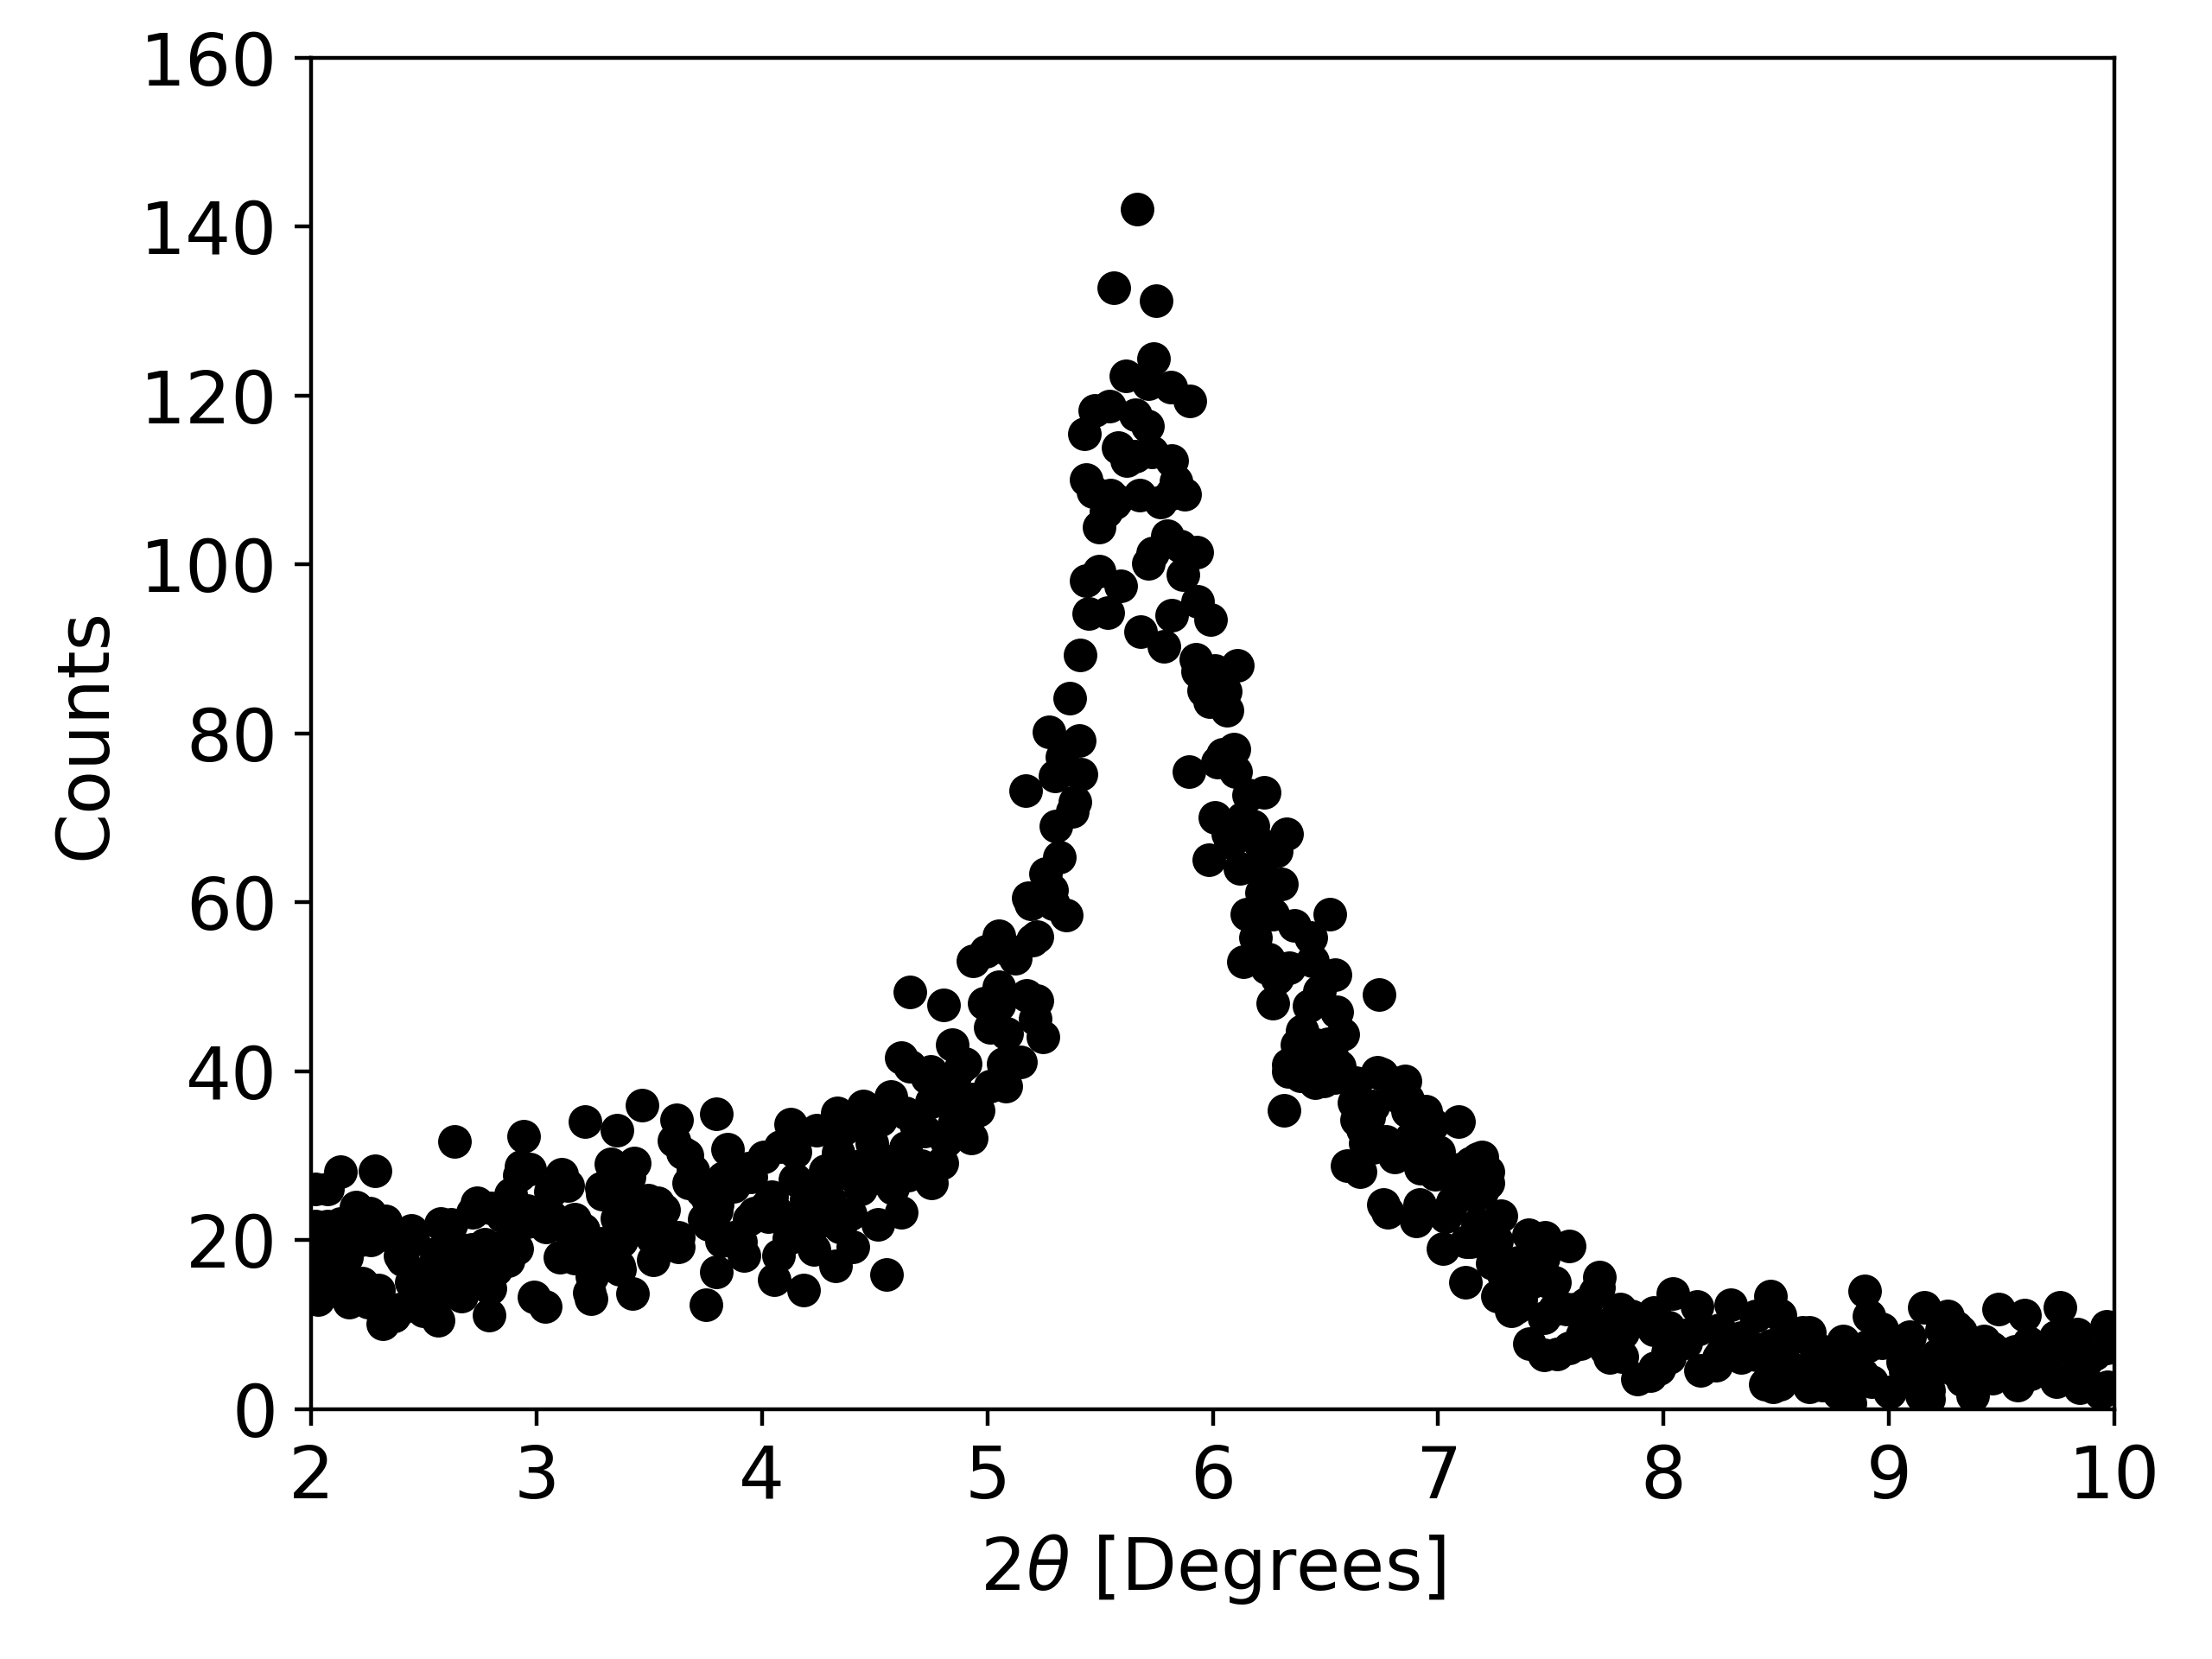
\includegraphics[scale=0.5]{images/97_pwd_5d.png}
		\caption{Initial scan, basal spacing of $d_{001}=15.5\angstrom$ and FWHM of $0.8^\circ$.}
		\label{fig:97_pwd_5d}
	\end{subfigure}%
	\begin{subfigure}{.5\textwidth}
		\centering
		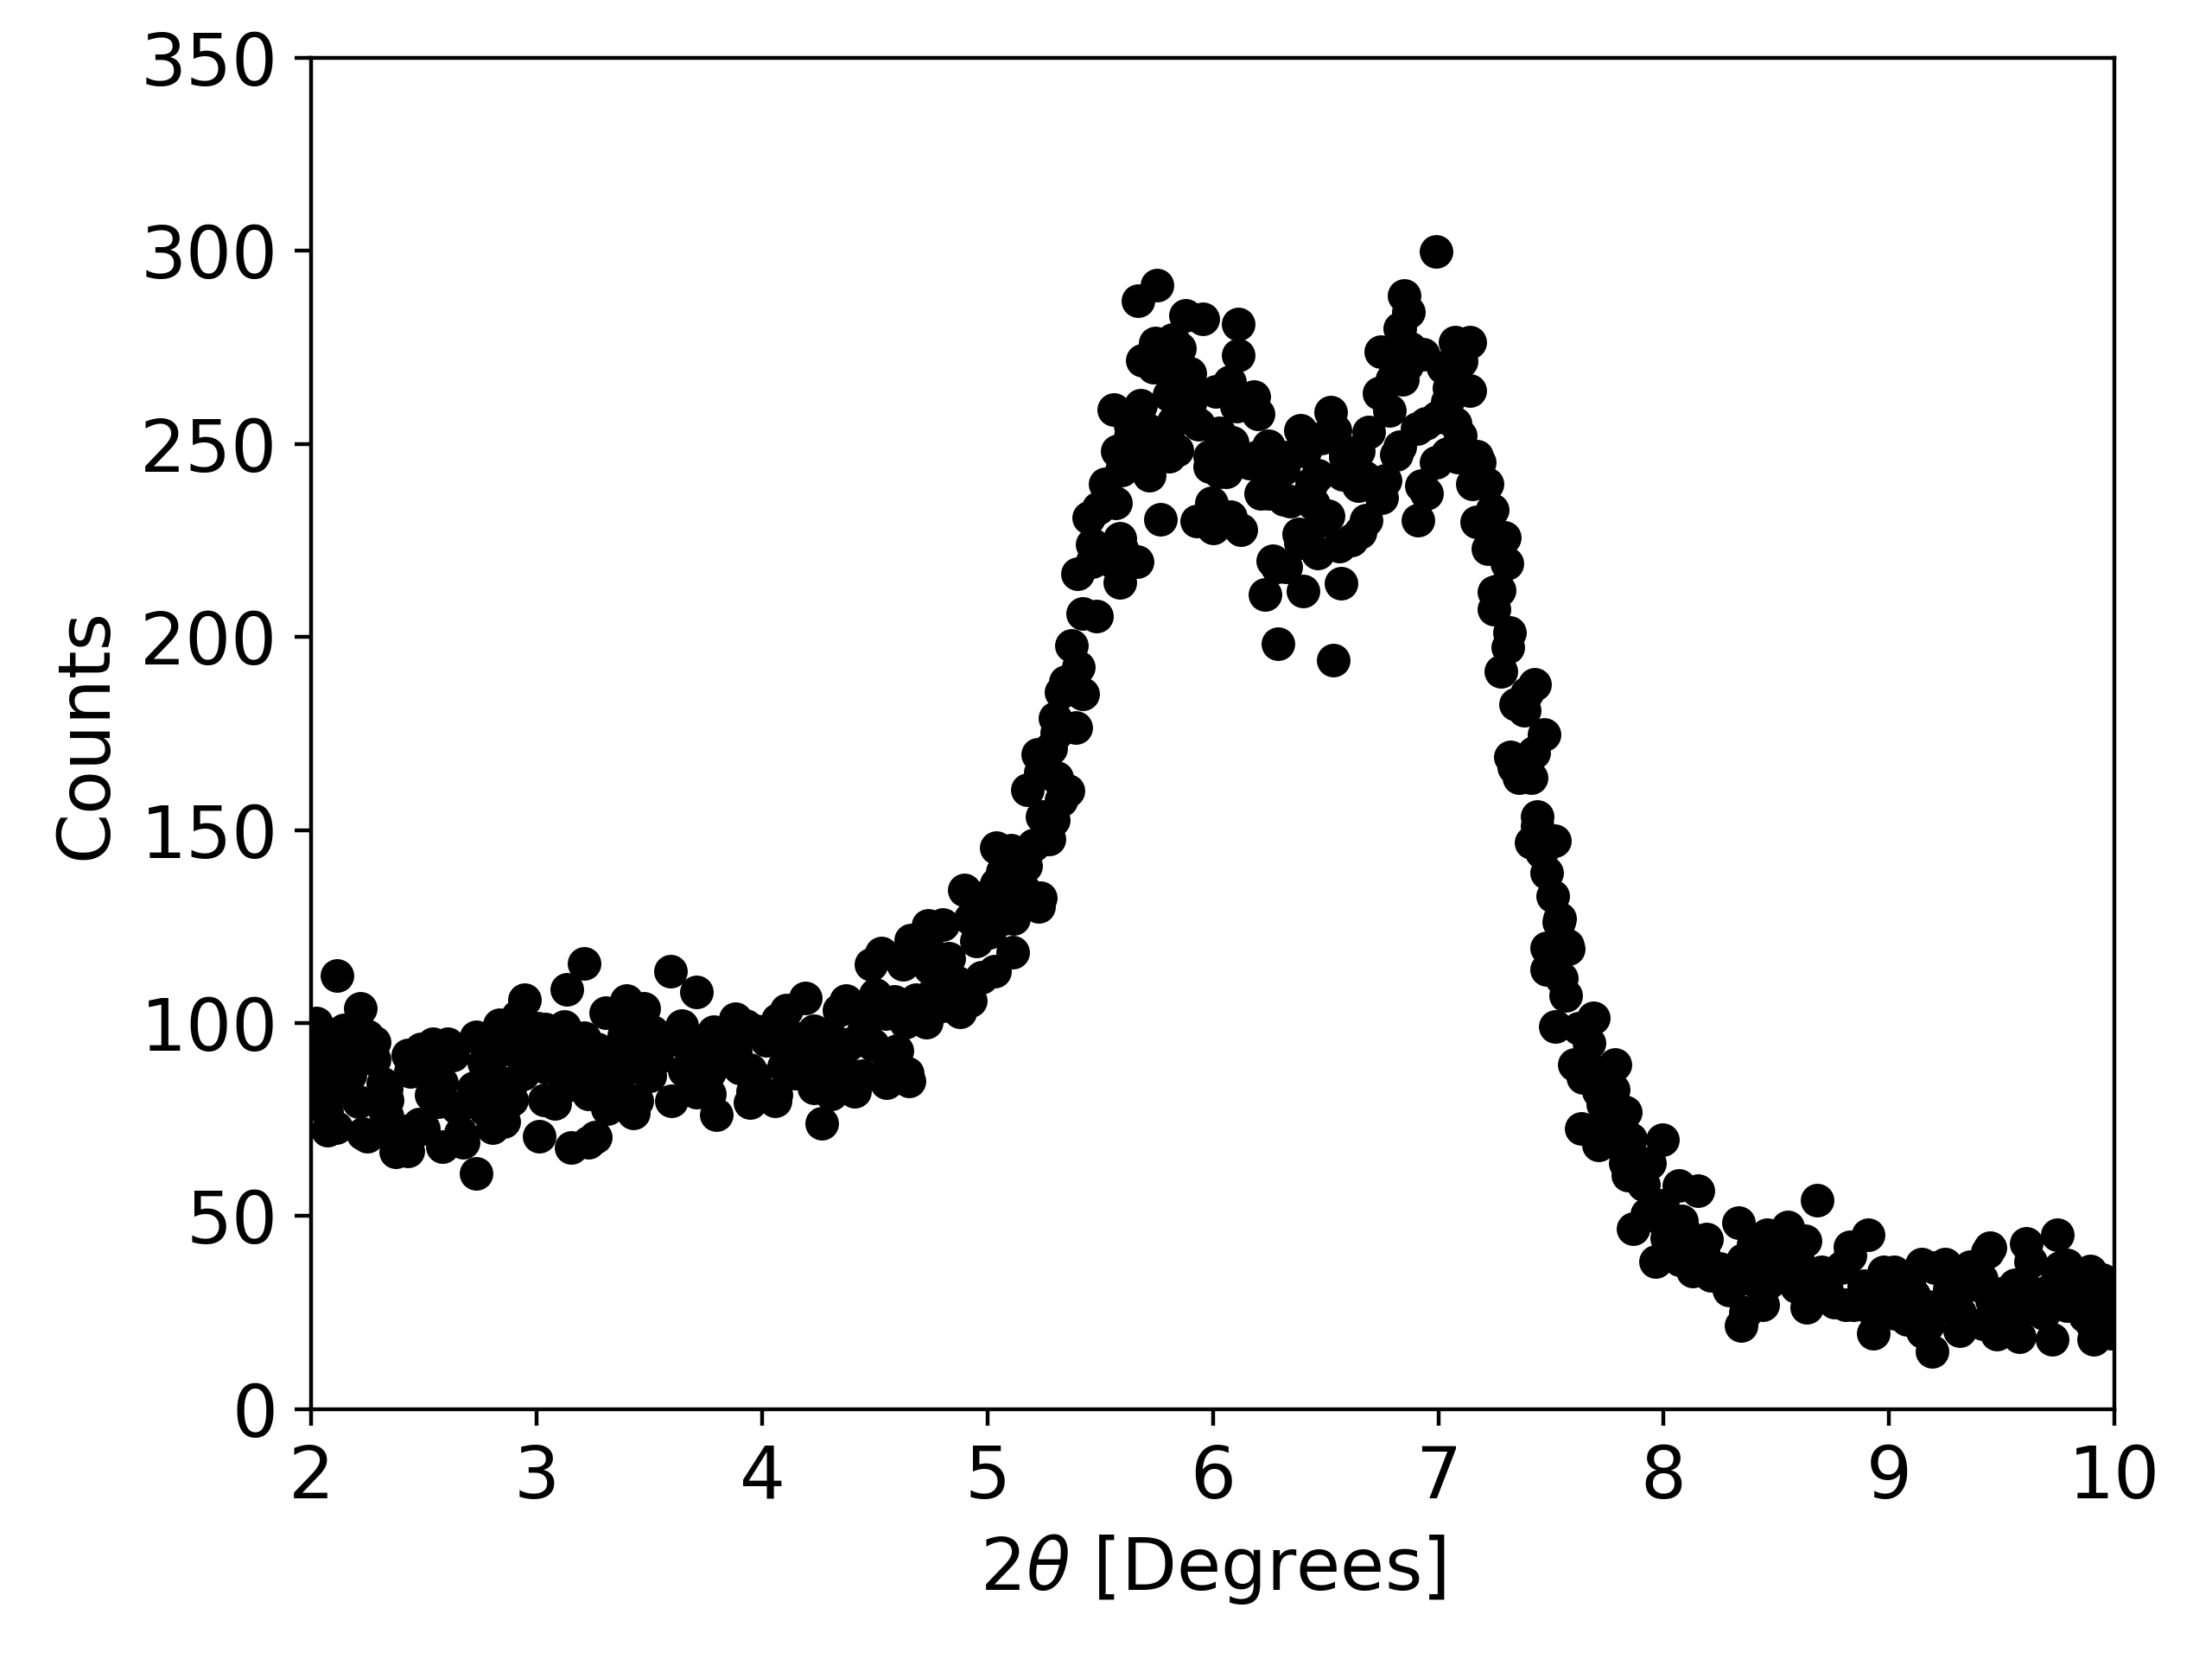
\includegraphics[scale=0.5]{images/97_pwd_5d_2.png}
		\caption{Second scan taken 15 minutes later. Peaks for spacing of $15.5\angstrom$ and $12.5\angstrom$.}
		\label{fig:97_pwd_5d_2}
	\end{subfigure}
	\caption{Bragg peaks of clay powder left in 97\% humidity for five days.}
	\label{fig:97_pwd_double}
\end{figure}

Upon increasing the duration for which the clay powder was left in the desiccator at 97\% humidity to five days, it was initially found that the sample had a near homogeneous bilayer of water intercalated between clay sheets. This peak may be observed in Figure~\ref{fig:97_pwd_5d}. There is a very small peak present at $7^\circ$, indicating some portions of the sample with only a monolayer, but the FWHM of the principal peak being less than $1^\circ$ indicated a very homogeneous bilayer hydration. While performing the scan however, which could take upwards of 20 minutes per sample, it was observed that the signal was changing with time. In Figure~\ref{fig:97_pwd_5d_2}, the signal of the exact same sample, but scanned 15 minutes later is presented. There is a very clear double peak, indicating that the sample now roughly has a 50\% bilayer and 50\% monolayer hydration. Observing this shift has shown just how sensitive the clay samples are to changes in the ambient relative humidity, and that while it may take the clay several days to obtain a homogeneous bilayer hydrate, this water may be lost in a matter of minutes if there is a large decrease in ambient humidity. Unfortunately, there is no way of knowing what the humidity in the XRD chamber was while these measurements were taken.

\subsubsection{Overview}
From this experiment, it is evident that the hydration of clay powder samples is much easier than that of the compressed clay pellets. This is likely due to the decreased surface area of clay which is in contact with the air for the clay pellets in comparison to the powder. It is also likely more difficult for the pellets to swell and expand due to their being too firmly compressed. More experiments would have to be conducted for longer periods of time to determine whether or not it is even possible to achieve a homogeneous bilayer hydration of a clay pellet. Such a task is manageable however if the clay is left in powder form, though the times required are much higher than those reported by Bérend et. al. \cite{berend1995mechanism}. Table~\ref{tab:hyd_time} provides a summary of the required times for different hydration levels. One reason for the greater times reported here is that the humidity inside of the desiccators might not have been that predicted by the prescribed salt solution. It is possible that the plastic desiccators used were not very airtight, or that there was not enough salt solution in each desiccator. Actually measuring the relative humidity is quite difficult, and requires expensive equipment which was not available. As such, all of the reported humidities in this work must be considered rough estimates at best. Despite this fact, these results should be easily reproducible with the specified salt solutions, and may even provide higher hydration levels in shorter periods of time if more salt solution or better desiccators are used.
\begin{table}
	\centering
	\caption{Times and humidities required for various hydration levels of Li montmorillonite.}
	\label{tab:hyd_time}
	\begin{tabular}{|c|c|c|c|}
		\hline
		\textbf{Humidity [$\bm{p/p_0}$]} & \textbf{Sample Type} & \textbf{Time [$\bm{hr}$]} & \textbf{Hydration} \\
		\hline
		\hline
		0.8 & pellet & 70 & monolayer \\
		\hline
		0.97 & pellet & 70 & monolayer, some bilayer \\
		\hline
		0.97 & powder & 70 & bilayer, large portion monolayer \\
		\hline
		0.97 & powder & 120 & bilayer \\
		\hline		
	\end{tabular}
\end{table}


%%% Local Variables: 
%%% mode: latex
%%% TeX-master: t
%%% End: 
 % chapter 2
%%%%%%%%%%%%%%%%%%%%%%%%%%%%%%%%%%%%%%%%%%%%%%%%%%%%%%%%%%%%%%%%%%% 
%                                                                 %
%                            CHAPTER THREE                        %
%                                                                 %
%%%%%%%%%%%%%%%%%%%%%%%%%%%%%%%%%%%%%%%%%%%%%%%%%%%%%%%%%%%%%%%%%%% 
 
\chapter{Infrared Spectroscopy of Clay Minerals}

\begin{figure}
	\centering
	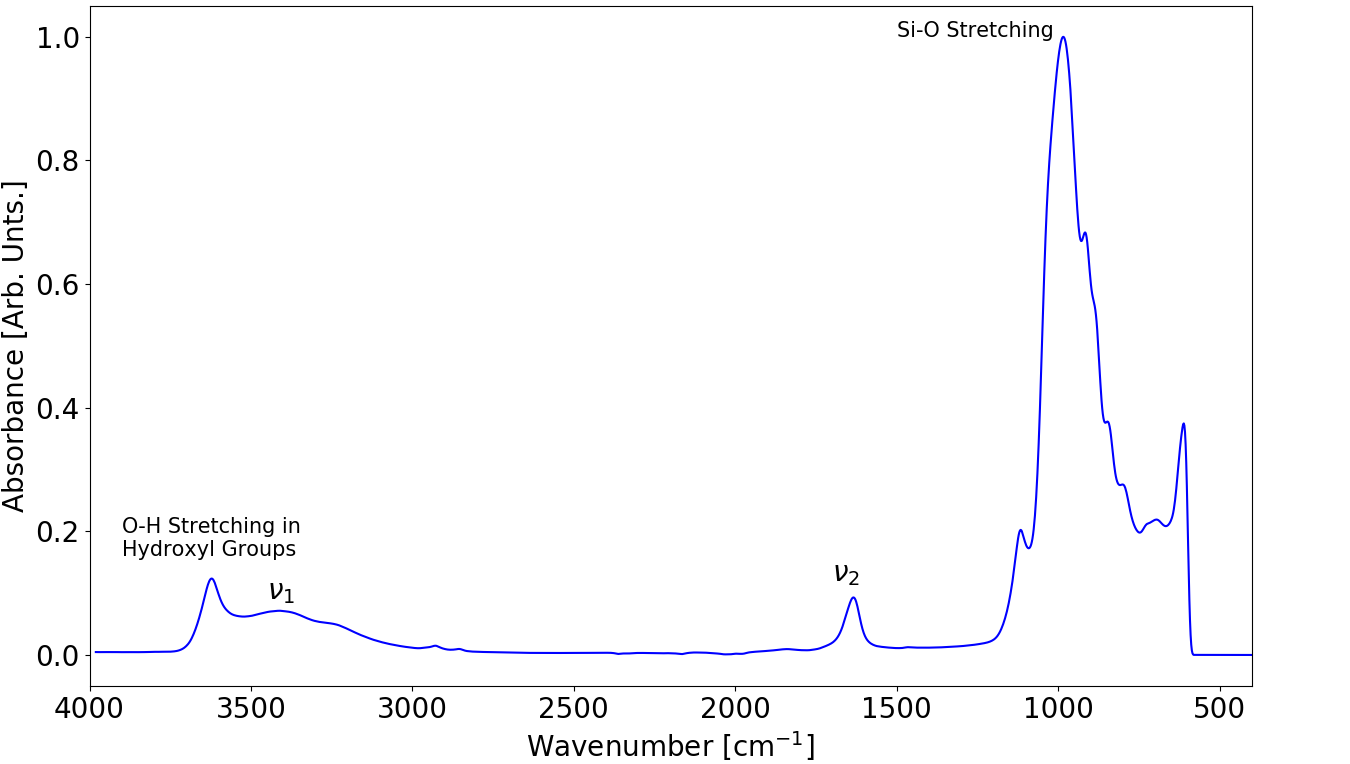
\includegraphics[scale=0.5]{images/spectrum_labels.png}
	\caption{Complete IR spectrum of a Li$^{\bm{+}}$ montmorillonite sample prepared at a pH of 7.}
	\label{fig:spectrum}
\end{figure}

\section{Infrared Spectrum of Montmorillonite}
An example of a typical infrared spectrum of a montmorillonite sample is provided in Figure~\ref{fig:spectrum}. In general, there are three regions of interest in the $500cm^{-1}$ - $4000cm^{-1}$ band. The first such region occurs between $500cm^{-1}$ and $1300cm^{-1}$. There are many overlapping absorbance bands within this region, all of which are attributed to vibrational modes of the clay structure itself. Within the scope of this work, these modes are of little interest, as we are focused primarily on the effects on water. It is also difficult to measure effects on these modes as their exact characteristics are heavily dependent on the composition, and therefore the source, of the clay samples \cite{madejova2001baseline}. One overarching trait of importance to this work however is the largest absorbance maximum in this region (and in the provided spectrum as a whole). This absorbance band is attributed to the Si-O stretching mode of the silica molecules in the clay \cite{madejova2001baseline}. This maximum is always the majorant over the spectrum, and is used in this paper to normalize our collected spectra, so that comparisons may be made between them. Apart from this, no analysis has been conducted on the absorbance bands located in this region.

Second, is the region between $1500cm^{-1}$ and $1800cm^{-1}$ containing one absorbance maximum, usually located at $1633cm^{-1}$. As previously mentioned, this is attributed to the bending mode of the intercalated water ($\nu_2$) \cite{madejova2003ftir}, \cite{madejova2001baseline}, \cite{bishop1994infrared}, \cite{johnston1992vibrational}, \cite{xu2000infrared}. This is one of the three bands which will be of interest for the remainder of this work.

\begin{figure}
	\centering
	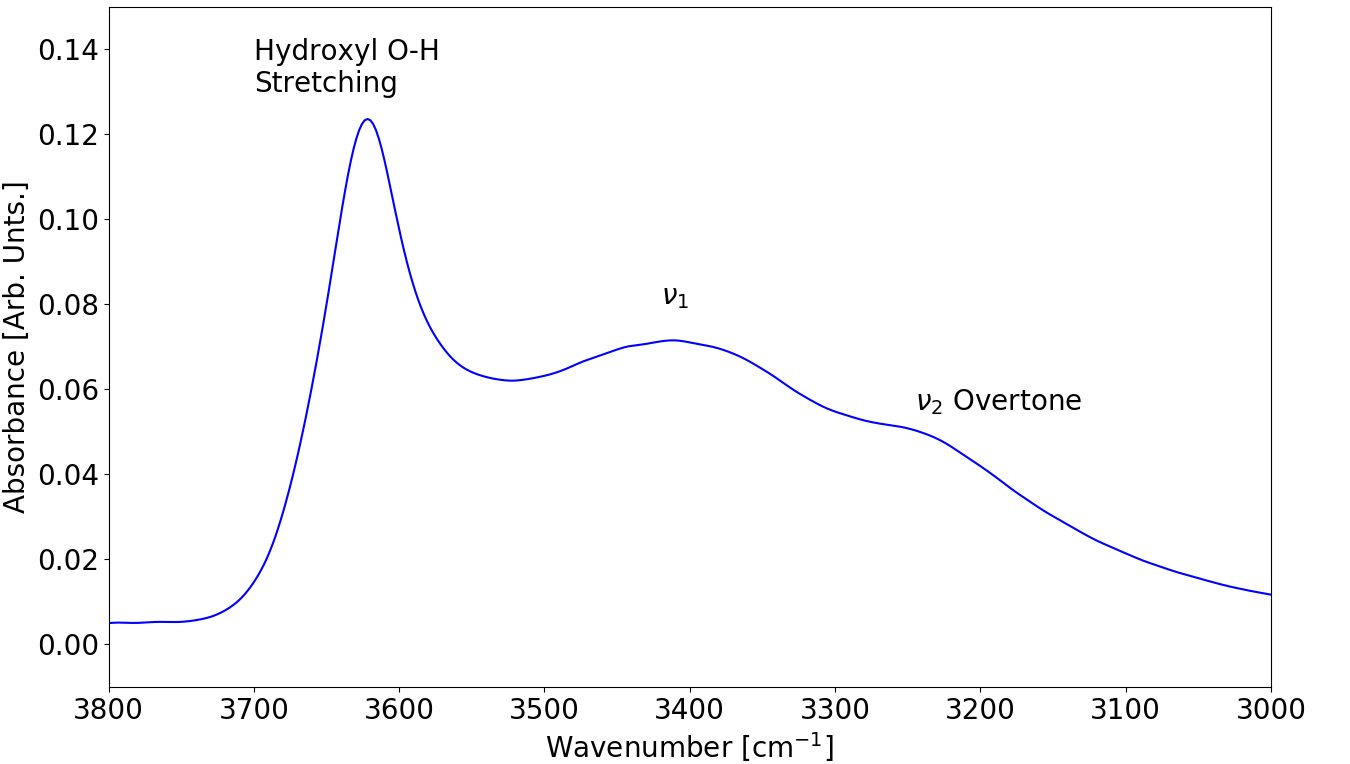
\includegraphics[scale=0.5]{images/water_peaks.png}
	\caption{3800cm$^{-1}$ - 3000cm$^{-1}$ region of montmorillonite infrared spectrum.}
	\label{fig:water_peaks}
\end{figure}

The third region of interest is between $3000cm^{-1}$ and $3800cm^{-1}$. In this band, there are three overlapping absorbance maxima. The most prominent and well defined is located at approximately $3620cm^{-1}$, and is attributed to the O-H stretching mode of the hydroxyl groups which are part of the clay lattice itself. The second which is much broader and located around $3410cm^{-1}$ is due to the symmetric stretching mode ($\nu_1$) of the O-H bond in the water molecules \cite{madejova2001baseline}. To the right, at $3242cm^{-1}$ is an overtone of the $\nu_2$ mode previously described \cite{xu2000infrared}. Of these three absorbance bands, the two which are pertinent to this work are the O-H stretching mode of the hydroxyl groups, and the $\nu_1$ mode of the intercalated water. Although the absorbance peak generated by the principal tone of the $\nu_2$ mode is tracked throughout the course of this experiment, the overtone was not considered in the analysis. This is due to the difficulty in fitting this small and less prominent absorbance peak, and because it is assumed that any variations in the $\nu_2$ mode of the water would present themselves in the resonance located at $1633cm^{-1}$.

Previously, it was briefly mentioned that all spectra collected in this work were normalized to the majorant absorbance peak of the Si-O stretching mode. While the structure and composition of montmorillonites varies (even within samples taken from the same location), it has been shown previously by Wilke, Aldersley, and Joshi that that the average compositions are similar enough that an appropriate choice for normalization would be the Si-O absorbance maximum \cite{wilke2016}. It is also easy to find and has a very consistent frequency between samples, making this an ideal choice as well. Normalizing the spectra is important, as the height of the absorbance maxima corresponding to $\nu_1$ and $\nu_2$ give an indication as to the quantity of water present, relative to other samples. The more water present in a sample, the higher the absorbance for the bands corresponding to modes occurring in the intercalated water. Therefore, as the level of hydration decreases, the heights of the $\nu_1$, $\nu_2$, and $\nu_2$ overtone absorbance bands also decrease \cite{madejova2003ftir}, \cite{bishop1994infrared}, \cite{johnston1992vibrational}, \cite{xu2000infrared}. While the height of these maxima and the hydration level of the clay are not specifically considered in this experiment, the effects of the hydration level on the frequencies of these vibration modes will be discussed in the upcoming section, and the ability to make general comparisons between spectra is of value.


\section{Previous Investigations}
\subsection{Effects of Hydration Level}
There have been many previous studies which examine the effects of hydration level on the stretching and bending modes of the intercalated water. Johnston, Sposito, and Erickson studied the effects of hydration on the water deformation mode ($\nu_2$) in their 1992 paper. In that work, it was found that regardless of which exchangeable cation was present in the clay sample, moving from a hydration level of 0 to approximately 10-15 H$_2$O molecules per cation, the frequency of the $\nu_2$ mode also increases. For a hydration of 15 or more H$_2$O molecules per cation, the frequency change begins to level off, and is similar to that of bulk water \cite{johnston1992vibrational}.

Bishop, Pieters, and Edwards in 1994 conducted a similar work, but expanded analysis to all bands attributed to water in the infrared and near infrared regions as well. Their results supported those of Johnston, Sposito, and Erickson, indicating that for Na montmorillonite, an observed shift in the $\nu_2$ band from $1617cm^{-1}$ to $1630cm^{-1}$ occurred as the sample was hydrated. Contrasting the behavior of the $\nu_2$ band, the absorbance maximum due to the $\nu_1$ band decreases with frequency as the hydration increases. No correlation was found between the band attributed to O-H stretching of structural hydroxyl groups and the hydration level \cite{bishop1994infrared}.

These two previous papers are further backed by a third, from 2000 written by Xu, Johnston, Parker, and Agnew. The results of Johnston's initial 1992 paper further support this work, and again show a trend of increasing frequency for the $\nu_2$ band from approximately $1625cm^{-1}$ to $1636cm^{-1}$ for Na and Li montmorillonites. At levels of hydration $>$ 10 water molecules per cation, the frequency again appears to remain constant. This paper also provided a more in depth analysis of the $\nu_1$ absorbance band as a function of water content as well. For all cations tested, the frequency of the symmetric stretching mode decreased with increasing water content. Na and Li samples tended to shift from around $3430cm^{-1}$ to $3420$ or $3415cm^{-1}$ when being hydrated from $<$ 5 water molecule per cation, to 15 molecules per cation. While this work did not specifically analyze the structural O-H stretching mode at $3620cm^{-1}$, based on their provided graphs, it would appear that little variation was present in this mode \cite{xu2000infrared}.

While specific values may vary slightly between these works, the general observations are consistent throughout. In general it is clear that more intercalated water causes an increase in the frequency of the $\nu_2$ mode, and a decrease in the frequency of the $\nu_1$ mode. Both the papers by Johnston and Xu propose the explanation that a decrease in the frequency of the $\nu_2$ mode under dehydration indicates that there are fewer hydrogen bonds forming between water molecules, and that the remaining molecules are then clustered around the exchangeable cations \cite{xu2000infrared}, \cite{johnston1992vibrational}. The paper by Johnston goes further in its explanation, stating that the water molecules conglomerated around the cation become polarized, and that this should be accompanied by an increase in the frequencies of the $\nu_1$ and $\nu_3$ modes \cite{johnston1992vibrational}. Though they were not able to make such observations at the time, the papers by Bishop and Xu both observe these traits in combination, supporting the provided explanation.

\subsection{Effects of Interlaminar Cation}
As previously explained, the amount of intercalated water has an effect on the frequencies of the symmetric stretching and deformation modes of this water. The interlaminar cation which is present also has an effect on these frequencies, due to both its size and valence. Furthermore, some of the previously discussed hydration properties may also be affected by the species of exchangeable cation present in the sample. Such effects shall briefly be discussed here.

In Johnston, Sposito, and Erickson's previously mentioned paper, the frequency range of the $\nu_2$ mode was examined at varying hydration levels for samples with Na, K, Co, and Cu cations. From their presented data it can be seen that upon reaching the hydration level at which the $\nu_2$ mode no longer changed with hydration, Co and Cu samples both had frequencies at approximately 1633$cm^{-1}$ to 1635$cm^{-1}$. These are slightly lower than the values for K and Na samples which were at 1637$cm^{-1}$ and 1640$cm^{-1}$ respectively \cite{johnston1992vibrational}. Bishop, Pieters, and Edwards observed that higher energies were observed for the water deformation mode for exchangeable cations which has a higher polarizing ability (i.e. higher charge and smaller radius). Similarly, it was postulated that as the polarizing ability of the cation is increased, the energy of the $\nu_1$ mode should decrease. This was supported in their observations for samples which had a higher water content, but for lower hydration levels, this appeared to not hold true \cite{bishop1994infrared}. Xu, Johnston, Parker, and Agnew also observed a strong dependence of the $\nu_2$ mode on the valence of the exchangeable cation. Na and Li samples reached a stable frequency at 1636$cm^{-1}$, while Mg and Ca samples were at slightly lower energies, of 1633$cm^{-1}$. For the $\nu_1$ mode, Na and Li samples had frequencies of approximately 3420$cm^{-1}$ at hydration of $>$ 10 $H_2O$ molecules per cation, while Ca and Mg samples were slightly lower, at 3415$cm^{-1}$ and 4505$cm^{-1}$ respectively \cite{xu2000infrared}.

With these direct effects due to the interlaminar cation described, one must also remember that the species of cation has an effect on the hydration level of the clay. As Jacques Méring described in his 1964 paper, montmorillonites which contain K as the exchangeable cation will usually only develop a monolayer of water between clay sheets. This is a general property as one moves down the periodic table, using cations with a larger radius, as compared to atoms such as Na and Li \cite{mering1964gonflement}. This difficulty in hydration means that the cation which is present could also lead to secondary effects which occur due to the hydration level, as discussed in the previous section.

\section{Effects of the Variation of pH}
To better understand the role the pH of a montmorillonite sample plays in this system, the following experiment was devised to better understand how the pH affects the symmetric stretching, and deformation modes of the water, and also of the O-H stretching mode in the structural hydroxide groups. To do this, series of samples were produced, with one series corresponding to one clay mine, and one exchangeable cation (Li, Na, or K). Within a series, 15 sample disks were produced, each corresponding to a different pH value between 3 and 10, using a 0.5 interval. Infrared spectra of each sample were then collected and analyzed. What remains of this chapter is devoted to an explanation of the methodology used, and the presentation of the results.

\subsection{Experimental Methods}
\subsubsection{Clay Sample Preparation}
The samples used through the course of this experiment were produced using montmroillonite acquired from the American Colloid Company, originating from the Belle Fourche A, C, and F clay mine beds, in addition to samples from the Miniota and Treherne mine beds. Homoionic samples with Li, Na, and K as the exchangeable cation were prepared by mixing the clays with chloride salts associated with the desired cation. All of the sample disks in a series were produced from the resulting clay, which was then titrated to the desired pH, using the methodology described by Banin et. al. \cite{banin1985ph}. After a sample at each desired pH level for a sample series was produced, the clay was centrifuged, then freeze dried, as prescribed by Aldersley, Joshi, Price, and Ferris \cite{aldersley2011role}.

With each series of clay powders produced, a clay pellet was produced for each pH in each sample series produced. The methodology used to produce these pellets is identical to that previously described in chapter 2. As before, no KBr was mixed with the clay powder. After each pellet was formed, it was placed in its own vial, and left in the lab at room temperature and room humidity ($p/p_0\approx 0.4 - 0.6$).

\subsubsection{Collection of Infrared Spectra}
For each sample prepared, two infrared spectra were taken using a Nicolet 4700 ATR-FTIR device. A resolution of 2$cm^{-1}$ was used for all measurements, and spectra were taken over the interval of $4000cm^{-1}$ - $500cm^{-1}$. To collect an infrared spectrum of a sample, the sample stage was first cleaned using isopropyl alcohol and disposable lab wipes. The desired clay pellet was then removed from its vial, and placed on the platform, and centered over the crystal. A press was then manually lowered onto the pellet, maintaining contact between the clay pellet and the crystal of the spectrometer. While the pellets are in general rather sturdy, the pressure required over the small surface area would sometimes cause the pellets to break in half, crumble, or crack. With a bit of finesse and practice, the maximum amount of pressure possible without breaking the clay pellet was applied. One may closely observe the surface of the pellet and see deformations and cracks begin to form, so it is known when to stop applying pressure. Despite the care used in this process, samples inevitably cracked, and crumbled. When this occurred, the press was removed, and the largest remaining piece of the sample was then placed over the crystal, and the press was again gently re-applied.

After one spectrum was completed, the press would be removed, and the sample (or its remains) would be reoriented to obtain a second spectrum in a different location on the pellet. After this, the sample and its remains would be collected and replaced in the vial. The stage and press would be washed again with isopropyl alcohol between each sample. Occasionally, a spectrum would be collected which did not resemble a standard infrared spectrum of montmorillonite. It was found that this was due to a lack of sufficient contact between the sample, and the spectrometer crystal on the stage. In this case, the sample was re-positioned, and more pressure was applied using the press.

\subsection{Results}

\subsubsection{Data Analysis}
\begin{figure}
	\centering
	\begin{subfigure}{1\textwidth}
		\centering
		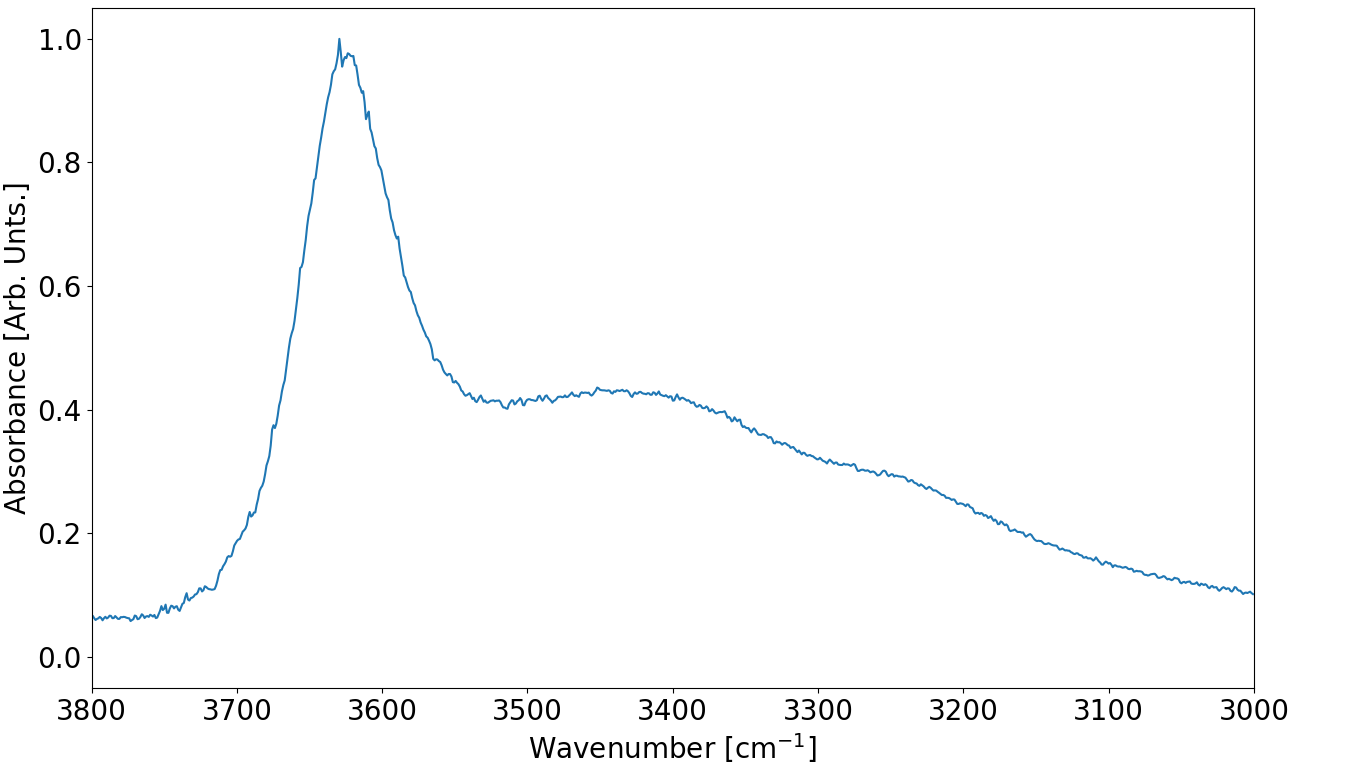
\includegraphics[scale=0.5]{images/raw_spectrum_noise.png}
		\caption{Raw sample spectrum with high frequency noise.}
		\label{fig:spectrum_noise}
	\end{subfigure}\newline
	\begin{subfigure}{1\textwidth}
		\centering
		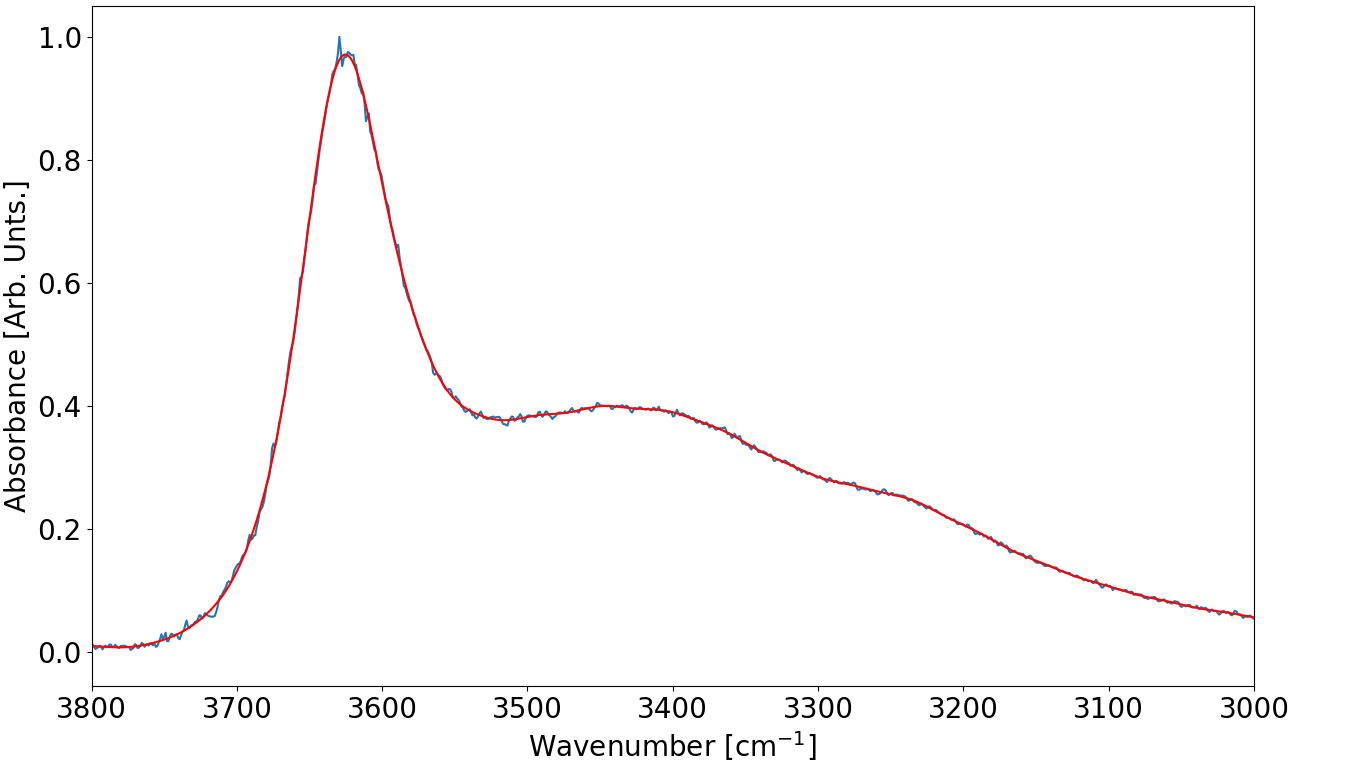
\includegraphics[scale=0.5]{images/filtered_peaks.png}
		\caption{Fourier filtered spectrum plotted over original spectrum from above.}
		\label{fig:filtered_specctrum}
	\end{subfigure}
	\caption{Raw and filtered spectrum of a pH 9.5 Na exchanged sample from 3800cm$^{-1}$ to 3000cm$^{-1}$.}
	\label{fig:raw_spectrum}
\end{figure}

Upon completion of scanning all samples twice, there were approximately 390 spectra which had to be analyzed. A resulting raw spectrum may be viewed in Figure~\ref{fig:spectrum_noise}. While this spectrum clearly has the overall characteristics of a montmorillonite infrared spectrum between 3000$cm^{-1}$ and 3800$cm^{-1}$, as initially presented by Figure~\ref{fig:water_peaks}, a high frequency noise is present in the spectrum. This noise made it difficult to pinpoint the frequencies of the $\nu_1$ and structural O-H stretching modes. Initially, a simple local averaging algorithm was used to smooth the data, but this lead to a slight loss of structure to the overall shape of the spectrum, especially in the region below 1000$cm^{-1}$, due to the number of small absorbance maxima in those areas. In an effort to preserve overall form, while also removing the high frequency noise, effectively smoothing the data, a Fourier filter was applied to the spectra. To accomplish this, the two regions of interest were each treated separately in the following manner: a linear background was subtracted from the region, using the end points of those regions. A Fourier filter was then applied, using a cutoff frequency of 0.024$cm$. This value was determined by trial and error, looking at the resulting form of the spectrum and adjusting the frequency until a spectrum which looked sufficiently smooth, while also conserving the overall form was found. Appendix~\ref{appendix:fft_filter} has the python script containing the Fourier Filter algorithm used. A filtered spectrum plotted over the original is provided in Figure~\ref{fig:filtered_specctrum}. As these filtered spectra were easier to find absorbance maxima locations from, they were used to conduct all the analysis, and find all frequencies.

Once filtered, the frequencies of the three local absorbance maxima of interest were obtained by fitting a Gaussian curve to the location of the maximum. Due to the large number of spectra collected and the time this would take to obtain all the data conducting the analysis by hand in software such as OriginPro, a script was written in Python to automate this process.

\subsubsection{Variations Due to pH}
\begin{figure}
	\centering
	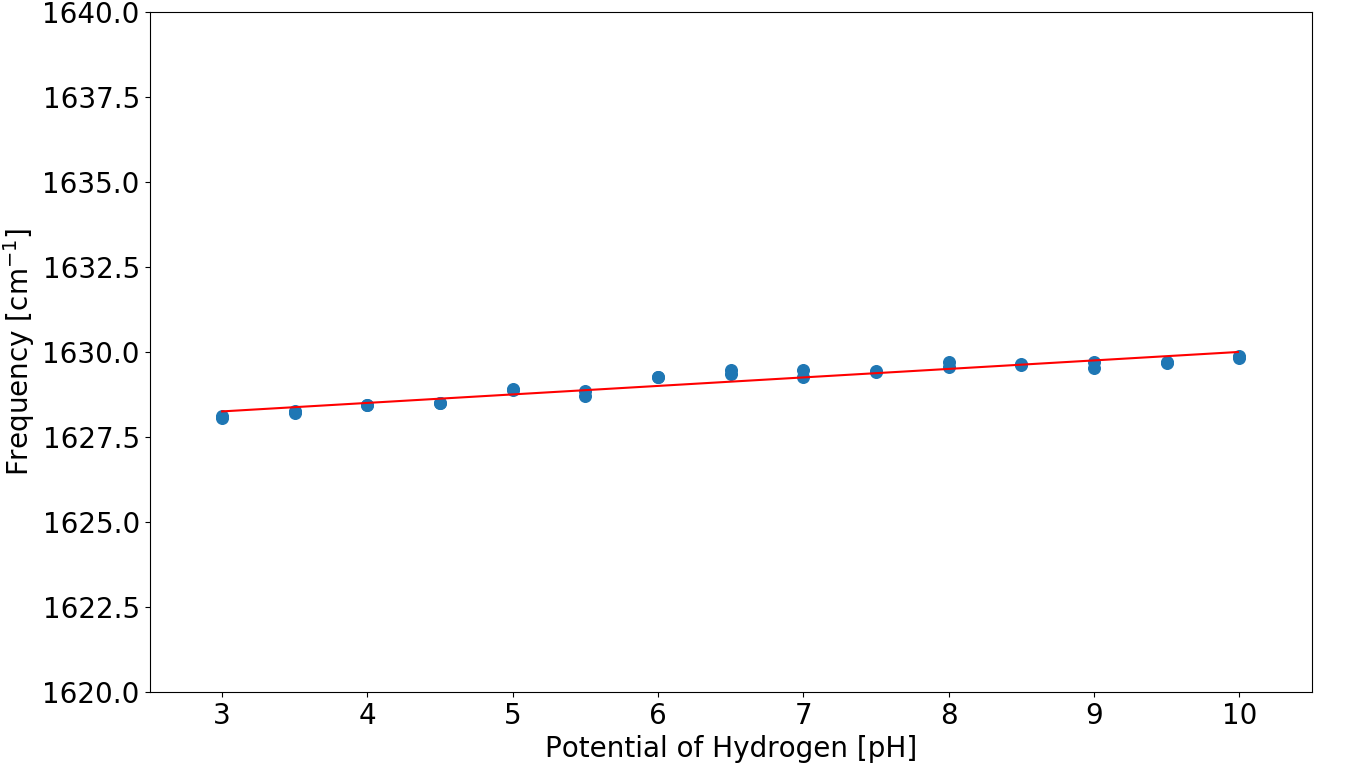
\includegraphics[scale=0.5]{images/deformation_shift.png}
	\caption{Water deformation mode of the Li sample series from Belle Fourche bed F as a function of the pH. Each 0.5 pH interval has two data points. Linear regression provided only as a guide to the eye.}
	\label{fig:deformation_shift}
\end{figure}
Once all the water vibration frequencies were determined for all samples in a series, the frequency of each of the three modes of interest was plotted against the pH of the sample. Looking at Figure~\ref{fig:deformation_shift}, one may see such a plot for the $\nu_2$ water deformation mode. From pH 3 to pH 10, there is an average shift in frequency of just under 2$cm^{-1}$. This observation was consistent between not only all Li sample series, but also for all series from the other two cations. One is directed to Table~\ref{tab:deformation_shifts} to see at what frequencies this shift occurred for each sample series.
\begin{table}
	\centering
	\caption{The frequencies over which the shift in the $\nu_2$ mode occurs when moving from pH of 3 to 10 for all sample series.}
	\label{tab:deformation_shifts}
	\begin{tabular}{|c||c|}
		\hline
		\textbf{Sample Series} & \textbf{Frequency Range of $\bm{\nu_2}$ Mode [$\bm{cm^{-1}}$]} \\
		\hline
		\hline
		Li $_A$ & 1628 - 1630 \\
		\hline
		Li $_C$ & 1628 - 1630 \\
		\hline
		Li $_F$ & 1628 - 1630 \\
		\hline
		Li $_T$ & 1628 - 1630 \\
		\hline
		Na $_A$ & 1628 - 1630 \\
		\hline
		Na $_C$ & 1628 - 1630 \\
		\hline
		Na $_F$ & 1628 - 1630 \\
		\hline
		Na $_M$ & 1628 - 1630 \\
		\hline
		Na $_T$ & 1628 - 1630 \\
		\hline
		K $_A$ & 1628 - 1630 \\
		\hline
		K $_C$ & 1628 - 1630 \\
		\hline
		K $_M$ & 1628 - 1630 \\
		\hline
		K $_T$ & 1628 - 1630 \\
		\hline
	\end{tabular}
\end{table}

\begin{figure}
	\centering
	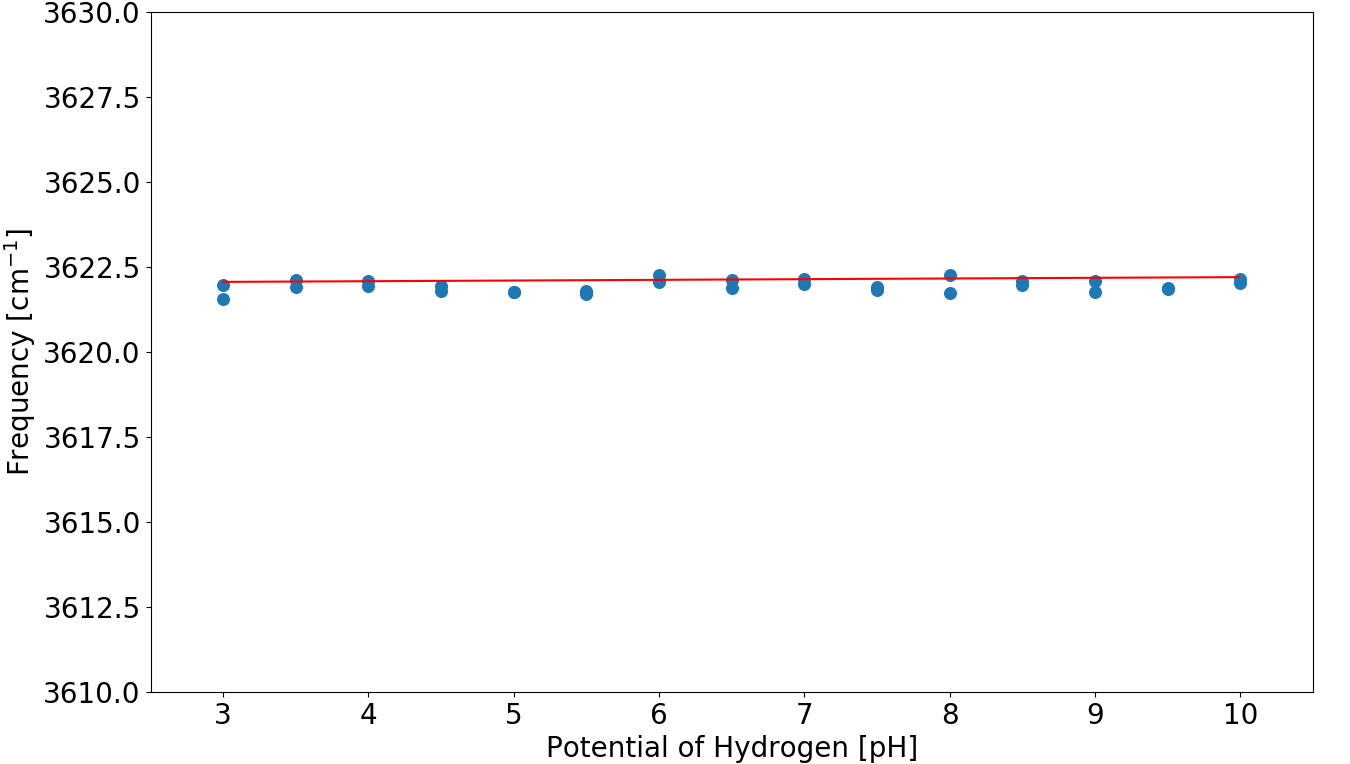
\includegraphics[scale=0.5]{images/hydrx_shift.png}
	\caption{Structural O-H stretching mode frequencies of the Li sample series from Belle Fourche bed F as a function of the pH. Each 0.5 pH interval has two data points. Linear regression provided only as a guide to the eye.}
	\label{fig:hydroxyl_shift}
\end{figure}

The observed shifts in the structural O-H mode had even fewer variations, remaining almost constant with changes in the pH. Figure~\ref{fig:hydroxyl_shift} demonstrates this for the Belle Fourche bed F, Li series. The line provided as a guide is notably more horizontal than for the previously mentioned $\nu_2$ mode. Same sample series were less constant however, having lower resonance frequencies at lower pH values. These differences were not usually more than 2$cm^{-1}$ from the max value which was quickly reached as the pH increased. The range of frequencies over which this mode was observed for each series may be found in Table~\ref{tab:structural_shifts}.

\begin{table}
	\centering
	\caption{The frequencies over which the shift in the structural O-H stretching mode occurs when moving from pH of 3 to 10 for all sample series.}
	\label{tab:structural_shifts}
	\begin{tabular}{|c||c|}
		\hline
		\textbf{Sample Series} & \textbf{Frequency Range of Structural O-H Mode [$\bm{cm^{-1}}$]} \\
		\hline
		\hline
		Li $_A$ & 3624 - 3625 \\
		\hline
		Li $_C$ & 3624 - 3627 \\
		\hline
		Li $_F$ & 3622 \\
		\hline
		Li $_T$ & 3621 - 3624 \\
		\hline
		Na $_A$ & 3624 - 3626 \\
		\hline
		Na $_C$ & 3626 - 3630 \\
		\hline
		Na $_F$ & 3622 \\
		\hline
		Na $_M$ & 3624 - 3626 \\
		\hline
		Na $_T$ & 3624 - 3625 \\
		\hline
		K $_A$ & 3624 - 3626 \\
		\hline
		K $_C$ & 3627 - 3630 \\
		\hline
		K $_M$ & 3624 - 3627 \\
		\hline
		K $_T$ & 3622 - 3626 \\
		\hline
	\end{tabular}
\end{table}

\begin{figure}
	\centering
	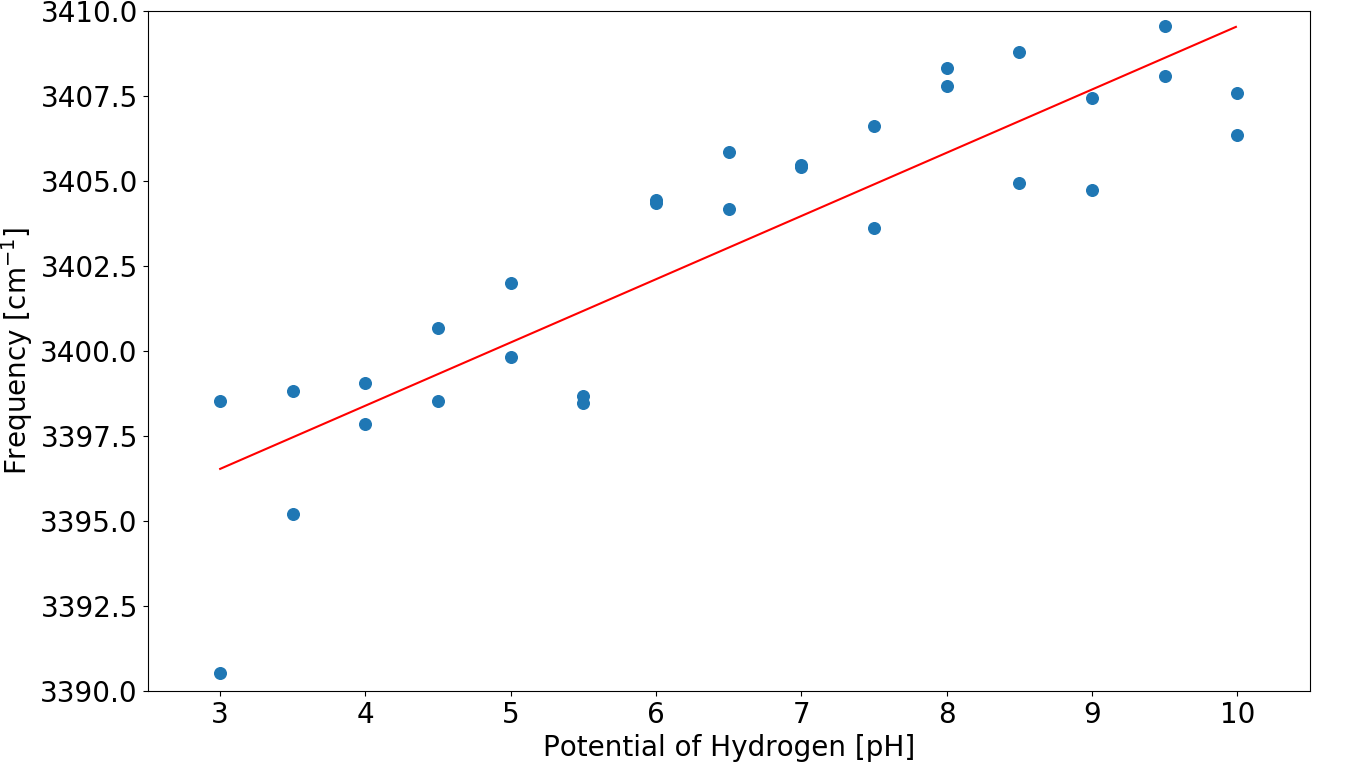
\includegraphics[scale=0.5]{images/water_shift.png}
	\caption{Symmetric O-H water stretching mode frequencies of the Li sample series from Belle Fourche bed F as a function of the pH. The linear regression is only provided as a guide to the eye.}
	\label{fig:water_shift}
\end{figure}
\begin{figure}
	\centering
	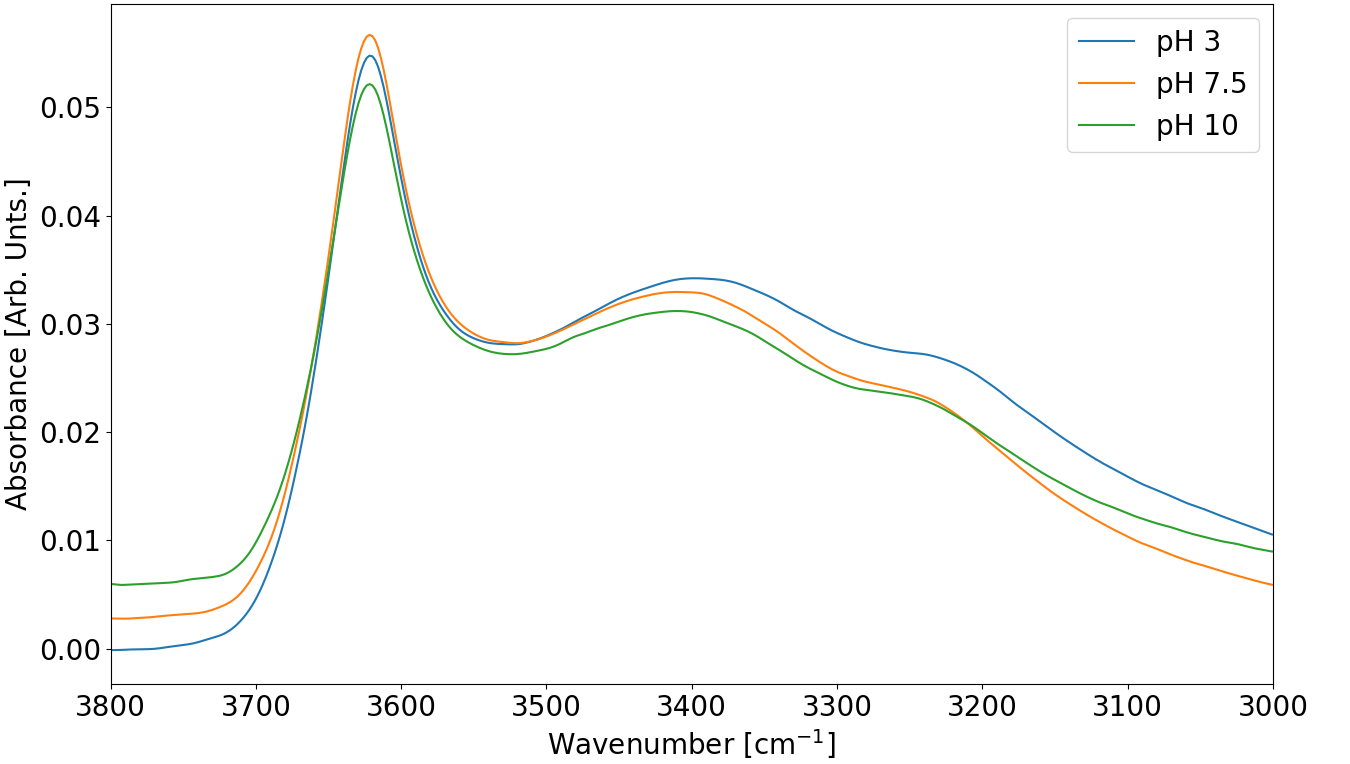
\includegraphics[scale=0.5]{images/spectra_shifts.png}
	\caption{Three spectra from the Belle Fourche F Li series, with visible shift in location of $\nu_1$ mode.}
	\label{fig:spectra_shift}
\end{figure}

We now arrive at the frequency shift of the $\nu_1$ mode as a function of pH, presented in Figure~\ref{fig:water_shift}. There are stark differences between this plot and the two immediately preceding it. The frequency of this mode clearly increases as the pH is increased from 3 to 10, by approximately 13$cm^{-1}$ in the presented case, much larger than the 2$cm^{-1}$ resolution. This general trend to increase in frequency was visible in all sample series for all exchangeable cations, and origin locations. Other Li sample series demonstrated much greater shifts though, sometimes 19$cm^{-1}$ or 25$cm^{-1}$ over the 3 - 10 pH range. A second visual outlining the shift in the $\nu_1$ mode is provided in Figure~\ref{fig:spectra_shift}. One can easily see how the smaller absorbance peaks attributed to the $\nu_1$ mode are not aligned, while the absorbance peaks for the structural O-H stretching mode are all perfectly aligned. Table~\ref{tab:stretch_shifts} provides the value for what was determined to be the average shift in frequency for the $\nu_1$ mode, determined by linear regression.

\begin{table}
	\centering
	\caption{Average frequency shifts for the three investigated modes of all Li sample series, found using linear regressions. The subscript represents which mine bed the series came from (Belle Fourche A,C,F, Treherne, and Miniota).}
	\label{tab:stretch_shifts}
		\begin{tabular}{|c||c|}
			\hline
			\textbf{Sample Series} & \textbf{Frequency Shift in $\bm{\nu_1}$ Mode [$\bm{cm^{-1}}$]} \\
			\hline
			\hline
			Li $_A$ & 13.99 \\
			\hline
			Li $_C$ & 25.76 \\
			\hline
			Li $_F$ & 13.04 \\
			\hline
			Li $_T$ & 19.18 \\
			\hline
			Na $_A$ & 22.73 \\
			\hline
			Na $_C$ & 20.33 \\
			\hline
			Na $_F$ & 17.77 \\
			\hline
			Na $_M$ & 40.08 \\
			\hline
			Na $_T$ & 30.27 \\
			\hline
			K $_A$ & 17.82 \\
			\hline
			K $_C$ & 7.72 \\
			\hline
			K $_M$ & 15.66 \\
			\hline
			K $_T$ & 33.43 \\
			\hline
	\end{tabular}
\end{table}

\subsection{Discussion}

From Table~\ref{tab:deformation_shifts}, one can see that all sample series had water deformation modes which occurred between 1628 and 1630 $cm^{-1}$. Typically, as with the Li series from Belle Fourche F bed,  the frequency of the $\nu_2$ mode had a slight shift, starting at the lower end of this 2$cm^{-1}$ band at pH 3, and moving to the 1630$cm^{-1}$ end at a pH of 10. Given the resolution was 2$cm^{-1}$, this slight shift can not be considered significant. That being said, most Li sample series displayed a similar trend as well, on the same order of magnitude. More experiments should be conducted to examine this region with a higher resolution, to see if this shift is of significance or not.

The frequency of the structural O-H hydroxyl group stretching had somewhat similar properties, in that the frequency remained quite constant over the range of pH values tested. At the lower range of tested pH values, this frequency was sometimes also lower than for the samples at higher pH values, by approximately 1 - 1.5 $cm^{-1}$. By pH values of 5 or higher, the frequency of this mode was constant, if it had appeared at lower frequencies for lower pHs. As the shifts were within the 2$cm^{-1}$ resolution of the measurements, and many series didn't have any measurable variation from the average value of the frequency, these slight shifts can not be considered significant. While the water deformation mode had the same frequencies for every sample series examined, the average frequency for the structural O-H stretching mode was not constant between sample series from different clay mines. At first glance one would think there is no trend. Upon further inspection however, it was realized that the frequency of this mode actually has a dependence on the clay mine, where the original clay powder for the samples was collected. Regardless of pH or exchangeable cation, series which came from the same clay mine tended to have very similar O-H stretching frequencies of their hydroxyl groups. Assuming clays which come from the same location have a similar structure in terms of substitutions and composition apart from the species of exchangeable cation, the exact frequency of this mode depends on the composition of the clay structure itself.

Shifts in the symmetric stretching mode of water, seen in Table~\ref{tab:stretch_shifts}, are blatantly different from the two previously examined modes however. While the deformation and the structural O-H stretching modes showed no significant variation with changes in the pH, the frequency of the $\nu_1$ mode did present with a variation which was visible in all sample series. Shifts ranging from 13$cm^{-1}$ up to 40$cm^{-1}$ were observed, often being ten times larger than the resolution. These shifts were obtained using a linear regression, though it should be noted that this method was used for its simplicity, and it not meant to describe any known theory. Regardless of cation species or clay mine, there was always a strong positive shift. It should be noted however that the correlation of the data was much better for the Li and Na sample series, than for the K series. This has been attributed to the K samples having less water, as previously discussed.


%%% Local Variables: 
%%% mode: latex
%%% TeX-master: t
%%% End: 
 % chapter 3
%%%%%%%%%%%%%%%%%%%%%%%%%%%%%%%%%%%%%%%%%%%%%%%%%%%%%%%%%%%%%%%%%%% 
%                                                                 %
%                            CHAPTER FOUR                         %
%                                                                 %
%%%%%%%%%%%%%%%%%%%%%%%%%%%%%%%%%%%%%%%%%%%%%%%%%%%%%%%%%%%%%%%%%%% 
 
\chapter{Molecular Dynamics Simulations of Clay-Water Interfaces}

	\section{Theoretical Background}
		Molecular dynamics simulations of the clay-water interface were performed to further investigate the experimentally observed trends in the behavior of the vibrational modes of the water molecules, and the pH of the system as seen in chapter three. Computational methods considering the classical and basic quantum mechanical effects have previously been developed and implemented in mature codes. The basic theory of these methods, and the setup of the simulated system are provided here. 
	
		
		\subsection{Traditional Force Field Approximations}
			The more traditional approach to molecular dynamics is to approximate the basic forces which act on atoms and molecules with well known and accepted functions to approximate such behaviors. The first source one must consider is the electrostatic force between atoms which are charged, or approximated as having a charge, which is modeled using the form of the Coulomb potential between two point charges:
			\begin{equation}
				U_{C_{ij}} = k_e \frac{q_iq_j}{r_{ij}}
				\label{eq:coulomb}
			\end{equation}
			where $k_e$ is the Coulomb constant. 
			
			The next force considered is the van der Waals force, between atoms in different molecules. Two common methods exist for approximating this force, being either the 12-6 or the 9-6 Lennard-Jones (LJ) potentials. In this work, we shall only make use of the 12-6 LJ potential, as this is the form used in the consistent valence force field (CVFF), which will be used in the subsequent simulations \cite{heinz2005force}. We arrive at a function describing these interactions of the form
			\begin{equation}
				U_{LJ_{ij}} = 4\epsilon_{ij}\bigg[ \bigg(\frac{\sigma_{ij}}{r_{ij}}\bigg)^{12} - \bigg(\frac{\sigma_{ij}}{r_{ij}}\bigg)^6\,\bigg]
				\label{eq:lj}
			\end{equation}
			with $\epsilon_{ij}$ being the depth of the potential well and $\sigma_{ij}$ being the distance at which the potential is zero, due to the repulsive and attractive components being equal to one another between atom $i$, and atom $j$. This force, along with the Coulomb potential shall be used to describe the intermolecular forces acting on any atom in a system.
			
			Lastly is the potential energy between bonded atoms, constituting the intramolecular forces at play. Under the CVFF (and the flexible water model discussed later), the intramolecular forces which dictate the bond distance, and bond angle are described using harmonic potentials.
			\begin{equation}
				U_{r_{ij}} = \frac{k_{r_{ij}}}{2}\big( r_{ij} - r_{0_{ij}} \big)^2
				\label{eq:bond_length}
			\end{equation}
			\begin{equation}
				U_{\theta_{ijk}} = \frac{k_{\theta_{ijk}}}{2}\big( \theta_{ijk} - \theta_{0_{ijk}} \big)^2
				\label{eq:angle}
			\end{equation}
			Equation~\ref{eq:bond_length} describes the length between bonded atoms $i$ and $j$, with $r_{0_{ij}}$ being the equilibrium distance, and $k_{r_{ij}}$ being the harmonic constant for that particular bond. Similarly, Equation~\ref{eq:angle} describes the potential energy stored in the angle formed by the bonded atoms $i$, $j$, and $k$. $\theta_{0_{ijk}}$ is the equilibrium angle, and $k_{\theta_{ijk}}$ is the spring constant for the formed angle. It should be remembered that while this potential is calculated between three atoms, it contributes no force on the atom situated at the vertex of the prescribed angle.
			
			The potential acting on any atom may then be described by the sum of all of these potentials, from all contributing atoms in the system. This particular combination is that used in the CVFF, and for the potential on any one atom, looks like
			\begin{multline}
				U_i = \underbrace{\sum_{j\:bonded}\frac{k_{r_{ij}}}{2}\big( r_{ij} - r_{0_{ij}} \big)^2 + \sum_{jk\:bonded}\frac{k_{\theta_{ijk}}}{2}\big( \theta_{ijk} - \theta_{0_{ijk}} \big)^2}_\text{intramolecular forces}  \\ + \underbrace{\sum_{j\:nonbonded}\bigg\{k_e \frac{q_iq_j}{r_{ij}} + 4\epsilon_{ij}\bigg[ \bigg(\frac{\sigma_{ij}}{r_{ij}}\bigg)^{12} - \bigg(\frac{\sigma_{ij}}{r_{ij}}\bigg)^6\,\bigg]\bigg\}}_\text{intermolecular forces}.
				\label{eq:potential}
			\end{multline}
			The force on an atom is then found taking the negative gradient of this function, which is then used to calculate a new velocity and position for the $i$th atom at each timestep \cite{heinz2005force}. Some physical intuition is the backbone of this approximation, and each term has an easily comprehensible physical meaning, adding to its poise and elegance, and also its completeness as this is a well accepted and well used form in the field of molecular dynamics simulations.
			
		\subsection{Reactive Force Field (ReaxFF) Approximation}
			The Reactive Force Field (ReaxFF) is a new method of performing molecular dynamics simulations, initially developed by van Duin, Dasgupta, Lorand, and Goddard. Desiring a method to simulate a more dynamic system, where chemical reactions and dissociation may occur, ReaxFF allows for bonds to be broken and formed through the course of the simulation, unlike the previously outlined traditional force fields which maintain all bonds, and do not allow new bonds to form. The potential energy is divided into different contributions, but many more components are involved such as calculating the bond order, under and over coordination, and other terms \cite{vanDuin2001reaxff}. This allows for complex interactions to be modeled, making ReaxFF a potentially very powerful force field. However, while being derived from well accepted physical principals, these terms are far more complex and lack basic intuitive physical meaning in contrast to the previously described force field. As such, outlining the equation for the potential energy would take far too long, and is outside the scope of this work. The inquisitive reader is thus encouraged to look at their original paper for a detailed outline of the ReaxFF implementation.
			
	\section{Simulation Methods}
	
		\subsection{Choice of Models}
			In order to perform a molecular dynamics simulation, it is necessary to have an initial data file, containing the starting locations of every atom, all bonds in the system, and all angles. Other bits of information are contained here as well, such as the spring constants, charges, well depths, and bond distances required to calculate the potential energy for each atom. In this sense, one not only needs the structure, but also the force field parameters. Montmorillonite poses a difficult system to model accurately, as there are many different types of bonds and angles which must be accurately determined in order to obtain reasonable simulation results. Hendrik Heinz from the University of Colorado Boulder however has produced just such system in his Interface Force Field (InterfaceFF), which provides force field parameters for many different compounds such as metals, and silicates including montmorillonite \cite{heinz2013thermodynamically}. This model has been shown to quite accurately model the interfacial properties of silicates, particularly with interactions with water \cite{emami2014force}. Many different force field parameters are provided in the suite, including the CVFF, which is one of the force fields to be used in these simulations.
			
			As the system to be modeled contains water which could undergo disassociation, it is worthwhile to consider a second model which considers chemical reactions as well. This was accomplished by combining a structure provided with the InterfaceFF, and using a ReaxFF potential which should be able to appropriately model the system in question. The chosen ReaxFF was that described by Pitman and van Duin in 2012, where they modeled interactions of water and Ca montmorillonite \cite{pitman2012dynamics}. Due to the fact that Ca is of a different valance than Na or K (the two cation species shipped with the InterfaceFF models), extensive changes to the charges on the clay surfaces of the model would be required to maintain neutrality. Given the difficulty of accomplishing this properly in the short time available, this force field was used with a different clay mineral model, kaolinite, which is also provided with the InterfaceFF suite. Kaolinite is also a swelling smectite, but lacks interlaminar cations, and has a 1:1 structure instead of a 2:1 like montmorillonite.
			
			Special attention must also be given to how the water in the system is modeled, as these vibrational modes are the primary quantity of interest. Perhaps the most popular is the simple point charge (SPC) model which has many different variations, but most are defined with rigid angles and bonds. Such a model would make it impossible to measure intramolecular vibrational modes. To get around this, the flexible water model proposed by Wu, Tepper, and Voth is used. This is an extension of the SPC model, in that the O-H bond length and the H-O-H angle are described with harmonic potentials, and the intermolecular forces are found using a 12-6 LJ potential \cite{wu2006flexible}. As these are all characteristic of the CVFF, it was decided that the CVFF model from the InterfaceFF system would be used to more easily integrate with the flexible water model, furthermore denoted as SPC/Fw.
			
		\subsection{Simulation Platform}
			All of the simulations were conducted using LAMMPS, freely distributed by Sandia National Labs \cite{plimpton1995fast}. This was compiled on a native Linux machine, including the following packages at compile: CLASS2, KSPACE, MOLECULE, USER-OMP, and USER-REAXC (\cite{aktulga2012parallel}). All simulations conducted in this work should be reproducible with these packages installed. Simulations were run in parallel, using all eight cores of an AMD FX-8350 CPU. Typical simulations required approximately one to two hours to run. In addition to this, there are three other pieces of software which were used through the course of this experiment. First is Packmol, which was used to create .pdb files which contained the initial distribution of water for the systems to be simulated \cite{martinez2009packmol}. Second was VMD, used for visualization of simulation models, and also converting .pdb files to LAMMPS data files \cite{humphrey1996vmd}. Another tool used for visualization was Ovito, which many will also find quite valuable \cite{stukowski2009Ovito}. Many other scripts were written by the author to aid in combining LAMMPS data files, changing atom properties, or performing analysis on the vibrational modes, all of which were written in Python, using the Python 2.7 standard. Familiarity with this language is therefore also of use.
			
		\subsection{Preparation of Input Data Files}
			\subsubsection{Clay Structures}
				For simulations using the CVFF, a montmorillonite structure was chosen from the InterfaceFF suite, and then combined with the distributed CVFF .frc file, also distributed with InterfaceFF, using the msi2lmp tool (provided with LAMMPS). This then produced a data file readable by LAMMPS containing all of the information for the clay structures. In running the msi2lmp command, the class I flag was used in the arguements, as CVFF is a class I force field. The structures used for the simulations were the Na montmorillonite 0.400 cell, and the K montmorillonite 0.333 5$nm$ neutral edge sheet.
				
				When using ReaxFF, the Kaolinite 15, single layer structure was used, as the atoms in this system were fully supported by the previously mentioned parameters from Pitman and van Duin. The structure was viewed with VMD, and output to a LAMMPS data file with just atoms positions. Force field parameters for ReaxFF are stored in a separate file, obtained from van Duin \cite{pitman2012dynamics}.
				
			\subsubsection{Water}
				As the water molecules must be placed between the layers of montmorillonite, Packmol was used to distribute them within a box, located between the two sheets. A single water molecule was defined in a .pdb, with the H atoms placed at their equilibrium positions, according to SPC/Fw model. Packmol then uses this to randomly orientate a given number of these molecules within the prescribed box. This .pdb file is converted to a LAMMPS data file using VMD, and the charges for the atoms, as well as the bond and angle definitions are added using a python script. The header of this file is manually updated ensuring the proper number of atoms, bonds, and angles. Pair coefficients, and parameters for bonds and angles are also added manually. These are the parameters defined in the paper describing the SPC/Fw model \cite{wu2006flexible}.
				
			\subsubsection{Combining Structures}
				LAMMPS has the capability to read multiple data files, but problems occurred in our simulations using this method, despite being sure to use the append and offset commands. To work around this, the clay structure and water molecules were simply combined into the same data file, with another python script. This ensured that atom and bond parameters were not over written and that both components of the simulation worked in the anticipated manner.
				
		\subsection{Simulation Parameters}
			Simulations were all run with periodic boundary conditions, with real units. Before simulations were started, particles were given randomly determined velocities, corresponding to the 300$K$, as all simulations were performed at 300$K$, and 1atm pressure (standard room temperature and pressure to match sample conditions). A timestep of 0.25$fs$ was employed, and most simulations were run for at least 200000 timesteps. A NPT thermostat and barostat were also used to maintain the temperature and pressure of the system. Simulations conducted using the CVFF used the sixth order mixing rule for parameter coefficients as opposed to geometric mixing rules due to the better results which are usually yielded \cite{waldman:1993cdd}. Examples of the LAMMPS input cards are provided in Appendix~\ref{appendix:cvff} and \ref{appendix:reaxff} with an example of a CVFF and a ReaxFF simulation card respectively. Table~\ref{tab:simulation_parameters_CVFF} provides the parameters used for the CVFF trials, while Table~\ref{tab:simulation_parameters_ReaxFF} provides the parameters used in the ReaxFF trials. In order to obtain the vibrational modes of the water, the ID, type, molecule number, and unwrapped positions of all atoms in the water were output at each timestep. Outputting this data at each timestep was done to increase the effective sample frequency when later finding the vibrational modes from the positions.
			
			\begin{table}
				\centering
				\caption{Provided below are the parameters used for all simulations conducted using the outlined CVFF traditional force field approach.}
				\label{tab:simulation_parameters_CVFF}
				\begin{tabular}{|c|c|c|}
					\hline
					\textbf{Simulation Parameter} & \textbf{Setting} & \textbf{Value}\\
					\hline
					Boundary Conditions & Periodic & \\
					\hline
					Units & Real & \\
					\hline
					Atom Style & Full & \\
					\hline
					\rule{0pt}{2.5ex} K-space Style & PPPM & 10$^{-6}$ \\
					\hline
					\rule{0pt}{2.5ex} Pair Style & lj/cut/coul/long & 12.0 $\angstrom$ $\qquad$ 8.0 $\angstrom$ \\
					\hline
					Bond Style & Harmonic & \\
					\hline
					Angle Style & Harmonic & \\
					\hline
					Dihedral Style & Harmonic & \\
					\hline
					Improper Style & CVFF & \\
					\hline
					Pair Coefficient Mixing Method & Sixth Power & \\
					\hline
					Thermostat & NPT & 300 $K$ \\
					\hline
					Barostat & NPT & 1 $atm$ \\
					\hline
					Timestep &  & 0.25 $fs$ \\
					\hline
					\hline
					\textbf{InterfaceFF Base Model} & \multicolumn{2}{c|}{\textbf{Description}} \\
					\hline
					\multirow{3}{*}{mont0\_400\_Na\_15\_cell} & \multicolumn{2}{c|}{Exchangeable Cation: Na$^+$} \\ & \multicolumn{2}{c|}{50 H$_2$O between two clay sheets} \\ & \multicolumn{2}{c|}{14040$\angstrom^3$ 1374 atoms} \\
					\hline
					\multirow{3}{*}{mont0\_333\_layer\_5nm\_neutral\_edges\_pH3} & \multicolumn{2}{c|}{Exchangeable Cation: K$^+$} \\ & \multicolumn{2}{c|}{100 H$_2$O on each side of one clay sheet} \\ & \multicolumn{2}{c|}{53143$\angstrom^3$ 3172 atoms} \\
					\hline
					
				\end{tabular}
			\end{table}
			
			\begin{table}
				\centering
				\caption{Provided below are the parameters used for all simulations conducted using the outlined ReaxFF approach.}
				\label{tab:simulation_parameters_ReaxFF}
				\begin{tabular}{|c|c|c|}
					\hline
					\textbf{Simulation Parameter} & \textbf{Setting} & \textbf{Value}\\
					\hline
					Boundary Conditions & Periodic & \\
					\hline
					Units & Real & \\
					\hline
					Atom Style & Full & \\
					\hline
					Pair Style & reax/c & NULL \\
					\hline
					Thermostat & NPT & 300 $K$ \\
					\hline
					Barostat & NPT & 1 $atm$ \\
					\hline
					Timestep &  & 0.5 $fs$ \\
					\hline
					\hline
					\textbf{InterfaceFF Base Model} & \multicolumn{2}{c|}{\textbf{Description}} \\
					\hline
					\multirow{3}{*}{kaolinite15\_single\_layer} & \multicolumn{2}{c|}{Exchangeable Cation: None} \\ & \multicolumn{2}{c|}{50 H$_2$O on one side of one kaolinite sheet} \\ & \multicolumn{2}{c|}{5616$\angstrom^3$ 660 atoms} \\
					\hline				
				\end{tabular}
			\end{table}
		
	\section{Analysis Methods}
		To the best of the author's knowledge, there is no adequate or reliable function or software to determine the vibrational mode within molecules in a LAMMPS simulation. Others have claimed to use the velocity auto correlation function (vacf) in LAMMPS, and then performed a Fourier transform on the data to obtain vibrational modes \cite{heinz2005force}. This method was attempted, performing the vacf function on the water molecules, but the results appeared to be nonsensical and no clear vibrational modes appeared to be present. Using the SPC/Fw model, this could not be the case and a new method was devised.
		
		At each timestep, the unwrapped position of each atom in the water was written to a dump file, along with its ID, and molecule number. Using this information, the vectors for the positions of each atom were defined as $\bm{r}_{_{H_1}}$, $\bm{r}_{_{H_2}}$, and $\bm{r}_{_O}$. From this, one is able to find the length of each O-H bond at each timestep with
		\begin{equation}
			r_{_{i}} = \abs{ \bm{r}_{_O} - \bm{r}_{_{H_i}} }.
		\end{equation}
		The angle formed by the molecule at each timestep is then found using
		\begin{equation}
			\theta = \cos^{-1}( \bm{\hat{r}}_{_{1}}\cdot\bm{\hat{r}}_{_{2}} ).
		\end{equation}
		With these quantities as functions of time, the vibrational modes were found by taking their Fourier transform. Because $\theta(t)$, $r_{_{OH_i}}(t)$ are oscillating about non-zero equilibrium values, complex magnitude of the Fourier transform will have large intensity low frequency components in the signal, making  it harder to measure the smaller components due to the vibrations of interest. To get around this, we subtract the average value ($\bar{\theta}$ and $\bar{r}_{_{OH_i}}$) from each function so that the transformed function is essentially oscillating about zero. In general, we calculate the Fourier transform of the angle (and likewise for the radial distance functions) with
		\begin{equation}
			F_\theta (\omega) = \int\limits_{0}^\infty \big[\theta(t) - \bar{\theta}\,\big]e^{-it\omega} \dd t.
		\end{equation}
		
		The magnitude of the Fourier transform ($\abs{F_\theta(\omega)}$) is used to determine the frequencies which are present in the signal. The added power of this method is that one may more easily identify from what vibration a given frequency is coming from, and isolate the signal, whereas computing a vacf for the entire system or just a certain group of atoms would make it very difficult to identify in which mode the frequency is present.
		
		\begin{figure}
			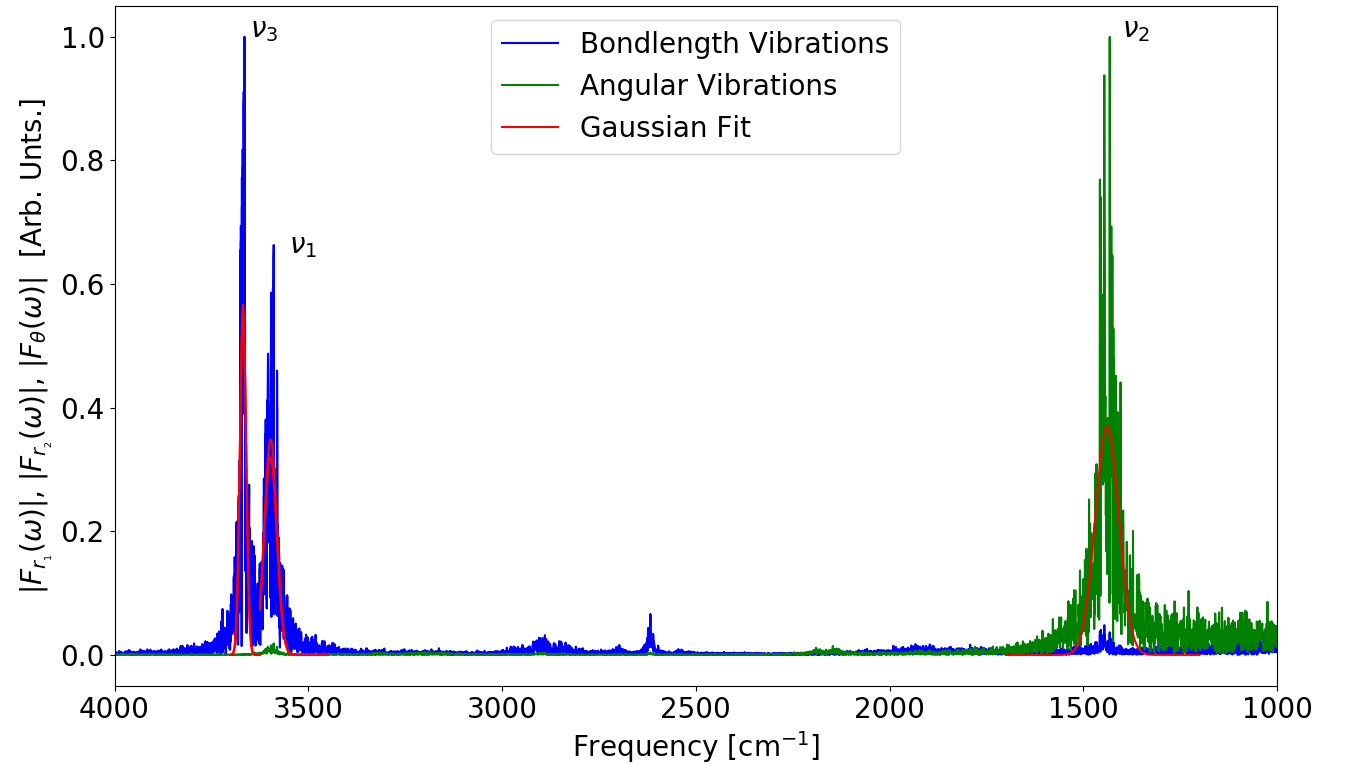
\includegraphics[scale=0.5]{images/Vibration_Modes.png}
			\caption{Normalized Fourier transforms for the O-H bond lengths and angle of a single water molecule in a Na montmorillonite simulation.}
			\label{fig:vib_modes}
		\end{figure}
		
		Figure~\ref{fig:vib_modes} depicts a resulting frequency spectrum. While the relative intensity between the $\nu_1$ and the $\nu_3$ modes is characteristic to their portions of the signal with respect to each other, the $\nu_2$ mode is calculated in such a way that one may not compare its intensity with that of the other two modes. It was possible to differentiate between the $\nu_1$ and $\nu_3$ modes by looking at the difference in their complex phases, which will be denoted as $\varphi(\omega)$.
		\begin{equation}
			\varphi(\omega) = \abs{\tan^{-1}\bigg( \frac{ \Im[F_{r_{_{1}}} (\omega)]}{\Re[F_{r_{_{1}}} (\omega)]} \bigg) - \tan^{-1}\bigg( \frac{ \Im[F_{r_{_{2}}} (\omega)]}{\Re[F_{r_{_{2}}} (\omega)]} \bigg)}
		\end{equation}
		When the frequencies appear in phase, their phase difference $\varphi$ should be near zero, while it should be approximately $\pi$ for two frequencies completely out of phase. Over the band at about 3700cm$^{-1}$, there was a phase difference of approximately $\pi$, while the phase difference in the band at 3550cm$^{-1}$ was approximately zero. One may see the plot of the phase difference in Figure~\ref{fig:phase} over this region.
		
		\begin{figure}
			\centering
			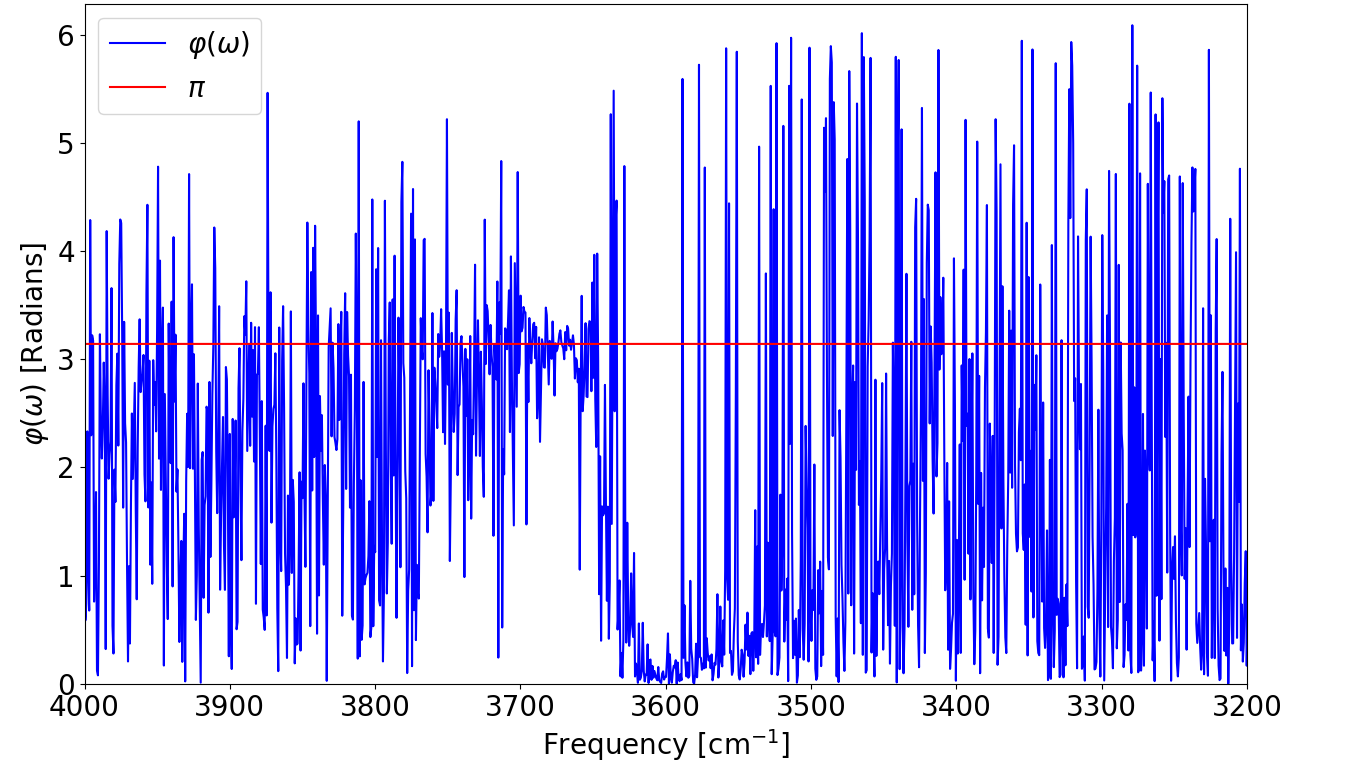
\includegraphics[scale=0.5]{images/phase.png}
			\caption{Phase difference in the Fourier transforms of the radial position of each hydrogen atom in the water molecule presented in Figure~\ref{fig:vib_modes}.}
			\label{fig:phase}
		\end{figure}
		
		For one simulation, the frequencies of the vibrational modes of each water molecule are determined, and then averaged over all molecules in the system.
	
	\section{Results}
		\subsection{ReaxFF Simulations}
		Reactions conducted using ReaxFF on one layer of kaolinite and one layer of water failed to relax appropriately. Even with the barostat and thermostat applied, large temperature and pressure oscillations were present. Upon visualizing the output in VMD, it was evident that the structure of the system degraded, and quickly lost any resemblance to the original structure. A solution to this problem was not found. It is possible that the force field used in this simulation was simply over parameterized to the system for which it was initially designed, or it was improperly implemented. Consequently, no data was collected using this method.
		
		\subsection{CVFF Simulations}
		The two models which were tested with the CVFF approach fared much better than the ReaxFF simulations. These models were able to maintain their structure, and relax to the prescribed 300K temperature. Slight oscillations in the pressure were observed; this is generally expected with large systems. The average frequencies for these two models are presented in Table~\ref{tab:frequencies}. Visualizations of the initial and final state of each system are provided in Figure~\ref{fig:na_visual} and Figure~\ref{fig:mont_visual}. The larger single layer of K montmorillonite appears to become two layers at the end, due to a rotation of the entire sheet within the simulation box, which is repeated due to the periodic boundary conditions. One may view the reported frequencies from the literature, and from this works experimental portions in Table~\ref{tab:frequency_comparison}. For both the $\nu_1$ and $\nu_2$ modes, the differences between the experimental and simulation frequencies are approximately 90$cm^{-1}$. It is possible that this is a constant difference in the model, but more trials and examinations will be required to see if this is the case.

		\begin{table}
			\centering
			\caption{Frequencies of water vibrational modes in CVFF simulations.}
			\label{tab:frequencies}
			\begin{tabular}{|c|c|}
			\hline
			\textbf{InterfaceFF Base Model} & \textbf{Average Frequencies} \\
			\hline
			\hline
			\multirow{3}{*}{mont0\_400\_Na\_15\_cell} & $\nu_1 = 3587 \pm 11\quad cm^{-1} $\\ & $\nu_2 = 1444 \pm 21 \quad cm^{-1}$ \\ & $\nu_3 = 3664 \pm \,\,\,6 \quad cm^{-1}$\\
			\hline
			\multirow{3}{*}{mont0\_333\_layer\_5nm\_neutral\_edges\_pH3} & $\nu_1 = 3588 \pm 12\quad cm^{-1} $\\ & $\nu_2 = 1443 \pm 26 \quad cm^{-1}$\\ & $\nu_3 = 3665 \pm \,\,\,6 \quad cm^{-1}$\\
			\hline
			\end{tabular}
		\end{table}

		\begin{table}
			\centering
			\caption{Frequencies obtained from literature and experimentation.}
			\label{tab:frequency_comparison}
			\begin{tabular}{|c|c|}
			\hline
			\rule{0pt}{2.5ex} \textbf{Frequencies From Madejova Baseline Study \cite{madejova2001baseline}} & \textbf{IR Experimental Results} \\
			\hline
			\hline
			\rule{0pt}{2.5ex} $\nu_1$ : 3373 - 3393 $cm^{-1}$ & $\nu_1$ : 3395 - 3420 $cm^{-1}$ \\
			\rule{0pt}{2.5ex} $\nu_2$ : 1629 - 1633 $cm^{-1}$ & $\nu_2$ : 1628 - 1630 $cm^{-1}$ \\
			\hline
			\end{tabular}
		\end{table}


		\begin{figure}
			\centering
			\begin{subfigure}{0.5\textwidth}
				\centering
				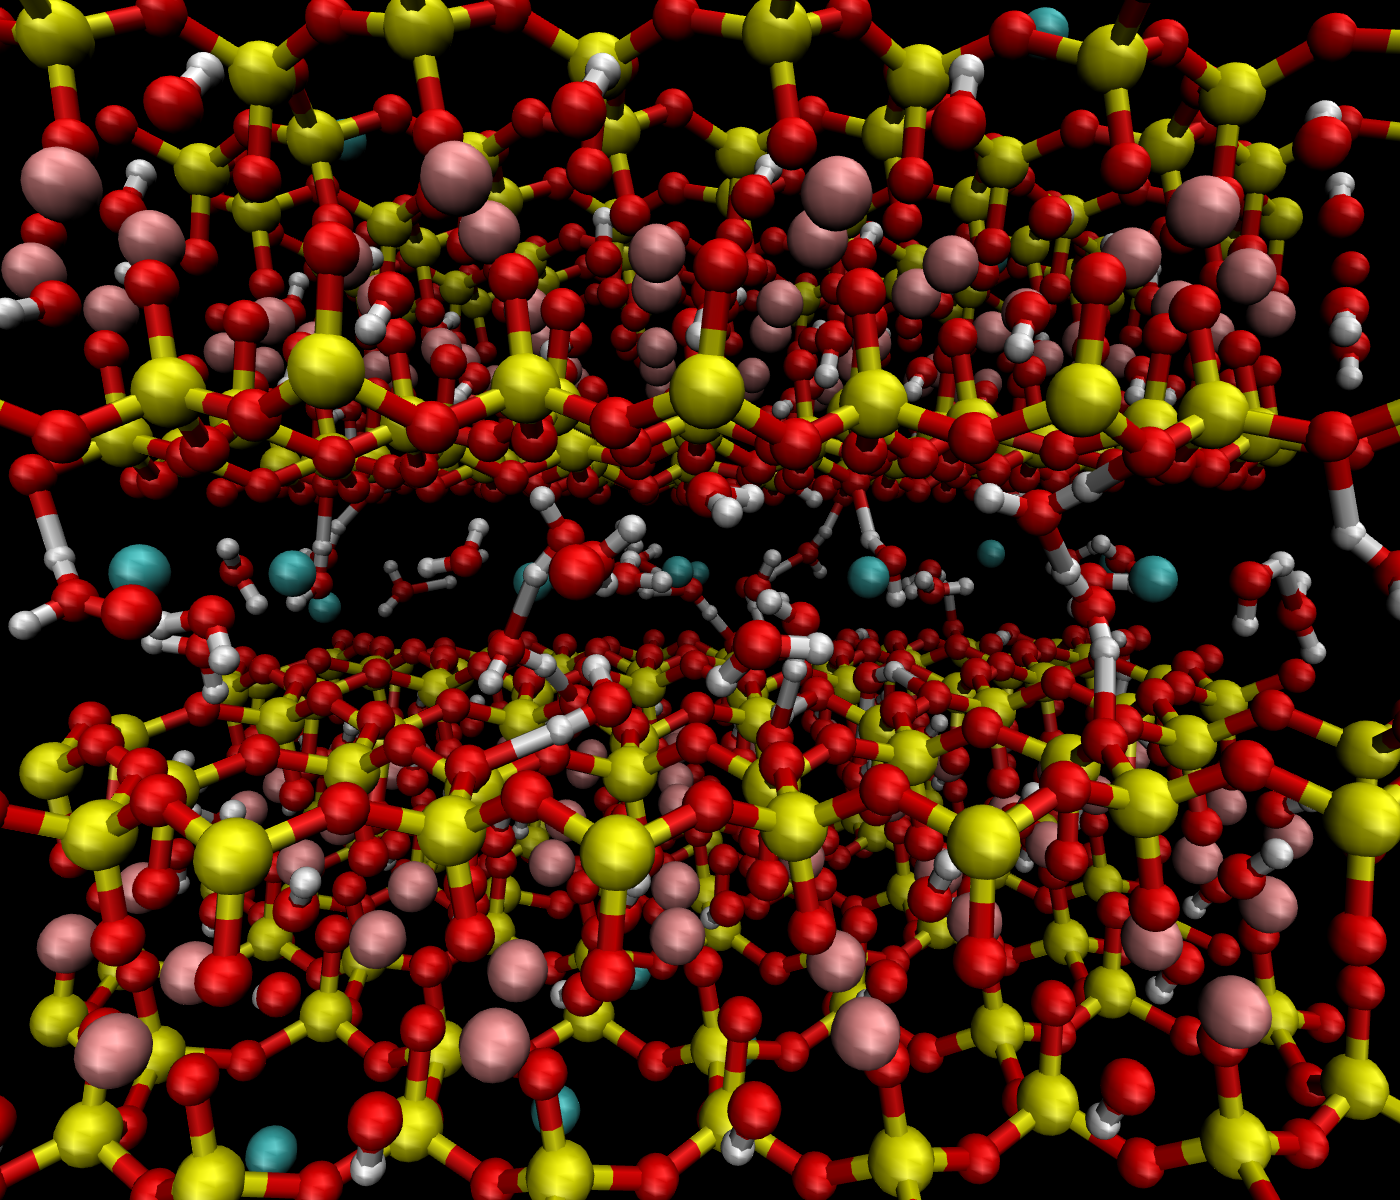
\includegraphics[scale=0.22]{images/na_init.png}
				\caption{Initial state}
			\end{subfigure}%
			\begin{subfigure}{0.5\textwidth}
				\centering
				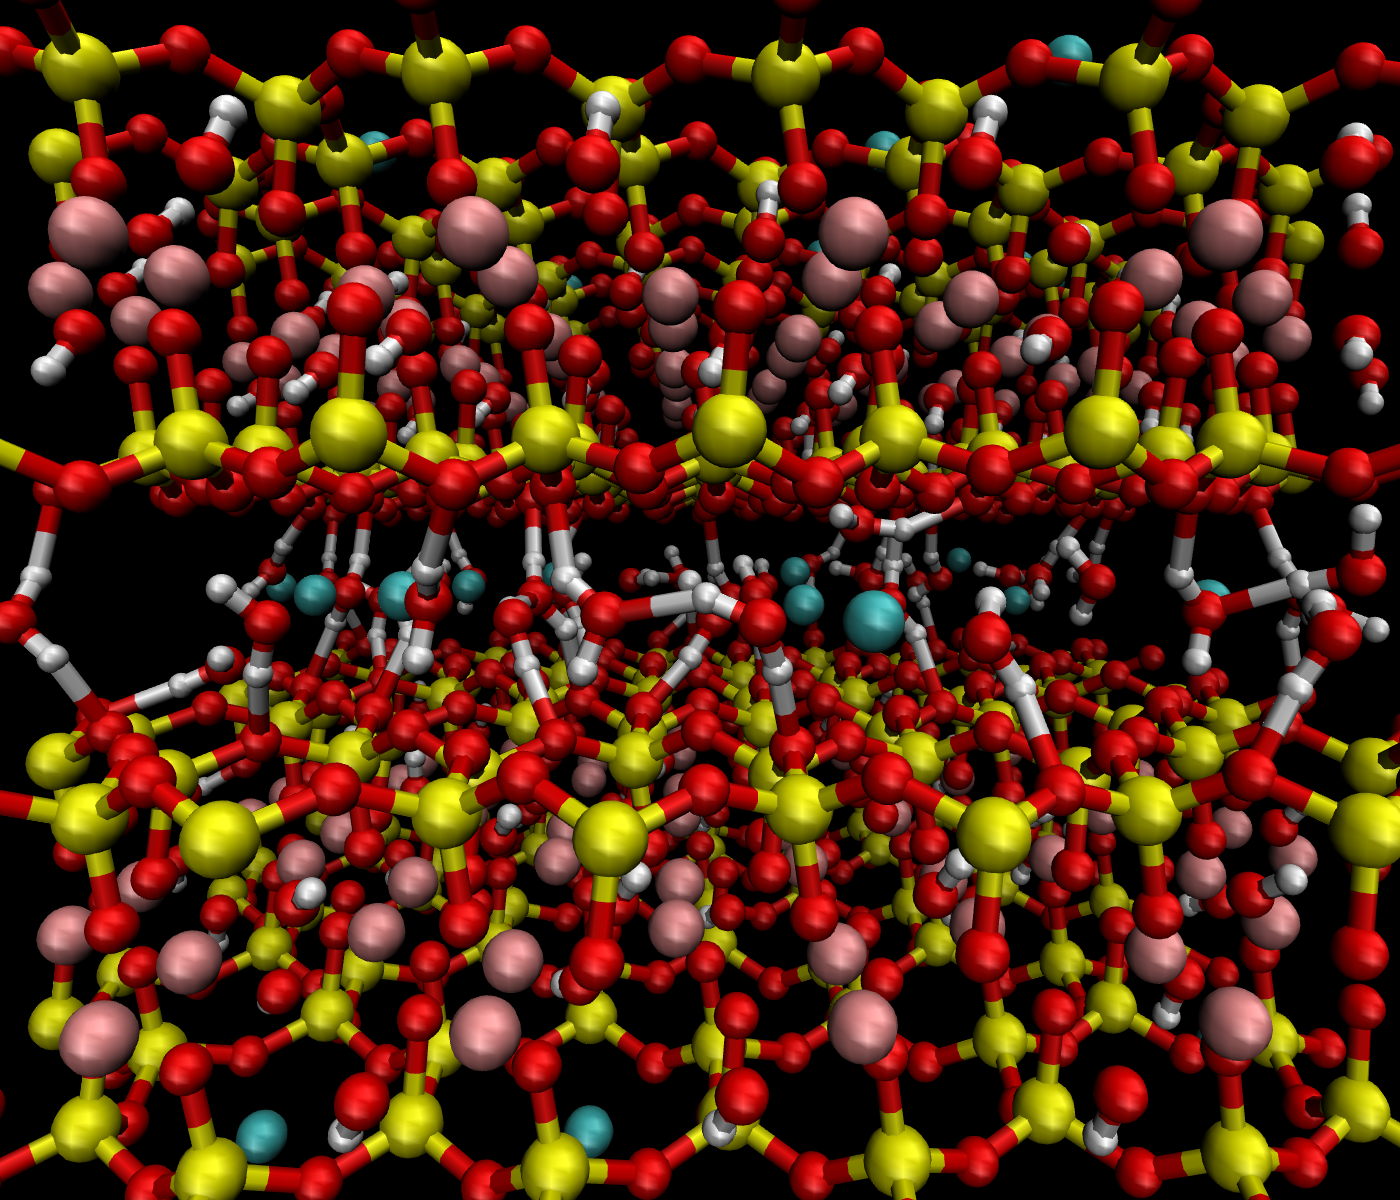
\includegraphics[scale=0.22]{images/na_fin.png}
				\caption{Final state}
			\end{subfigure}
			\caption{VMD Visualizations of Na montmorillonite cell simulation.}
			\label{fig:na_visual}
		\end{figure}
		
		\begin{figure}
			\centering
			\begin{subfigure}{0.5\textwidth}
				\centering
				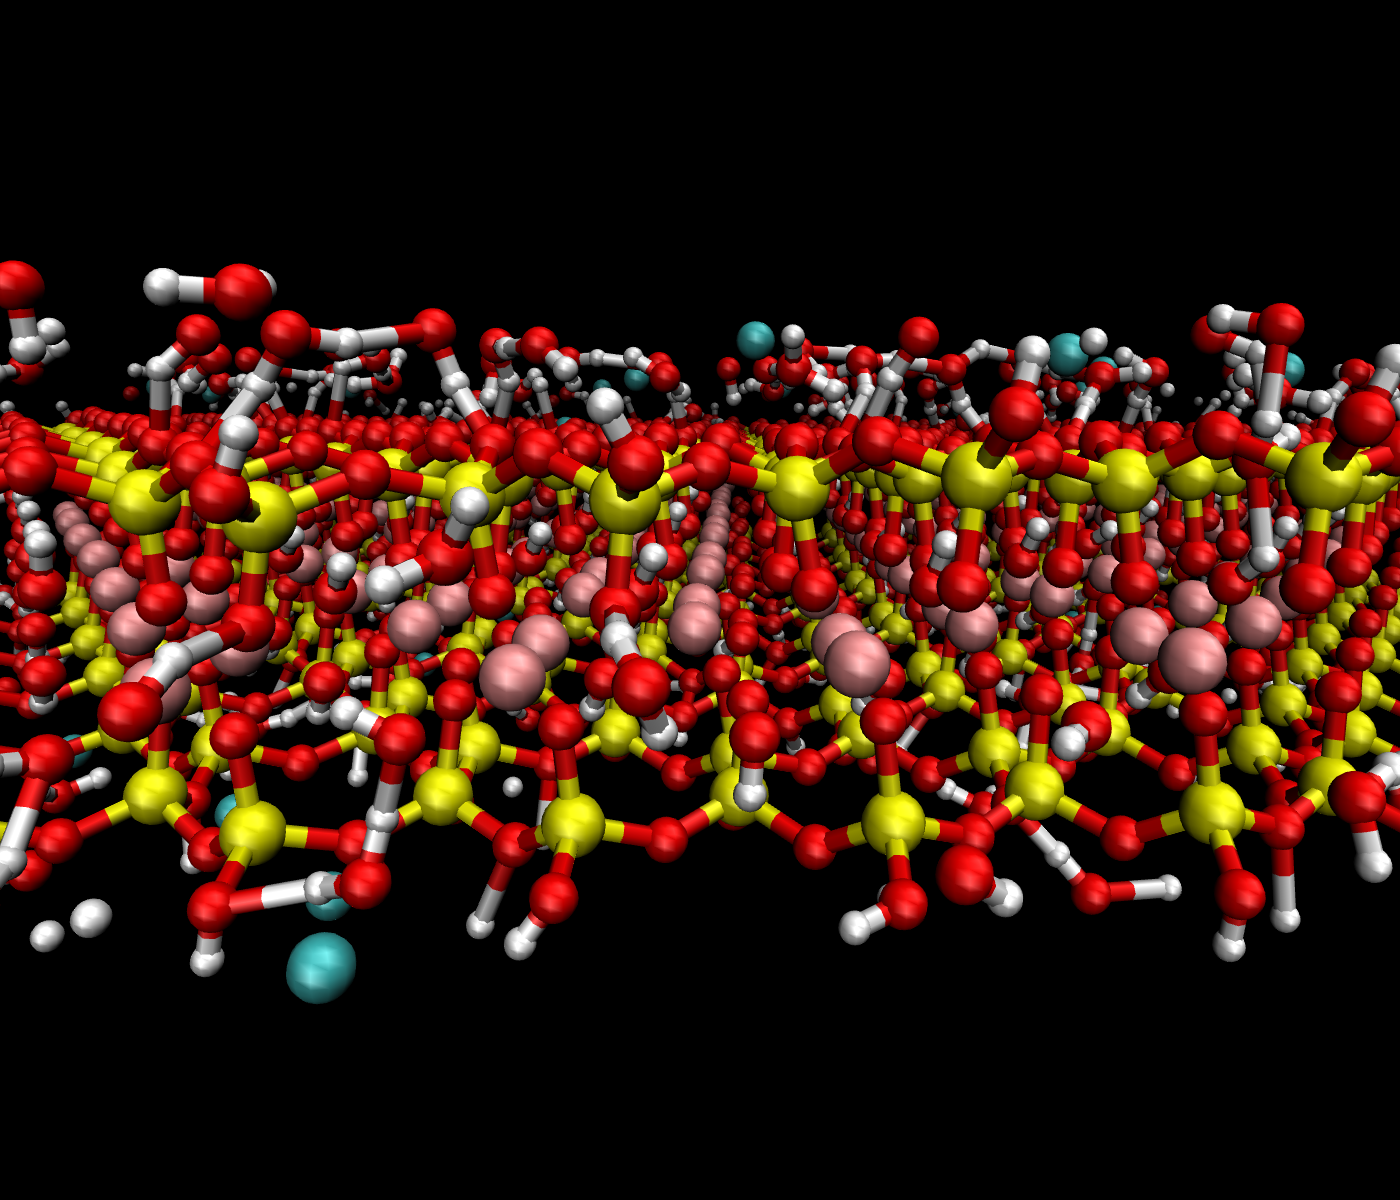
\includegraphics[scale=0.22]{images/mont_init.png}
				\caption{Initial state}
			\end{subfigure}%
			\begin{subfigure}{0.5\textwidth}
				\centering
				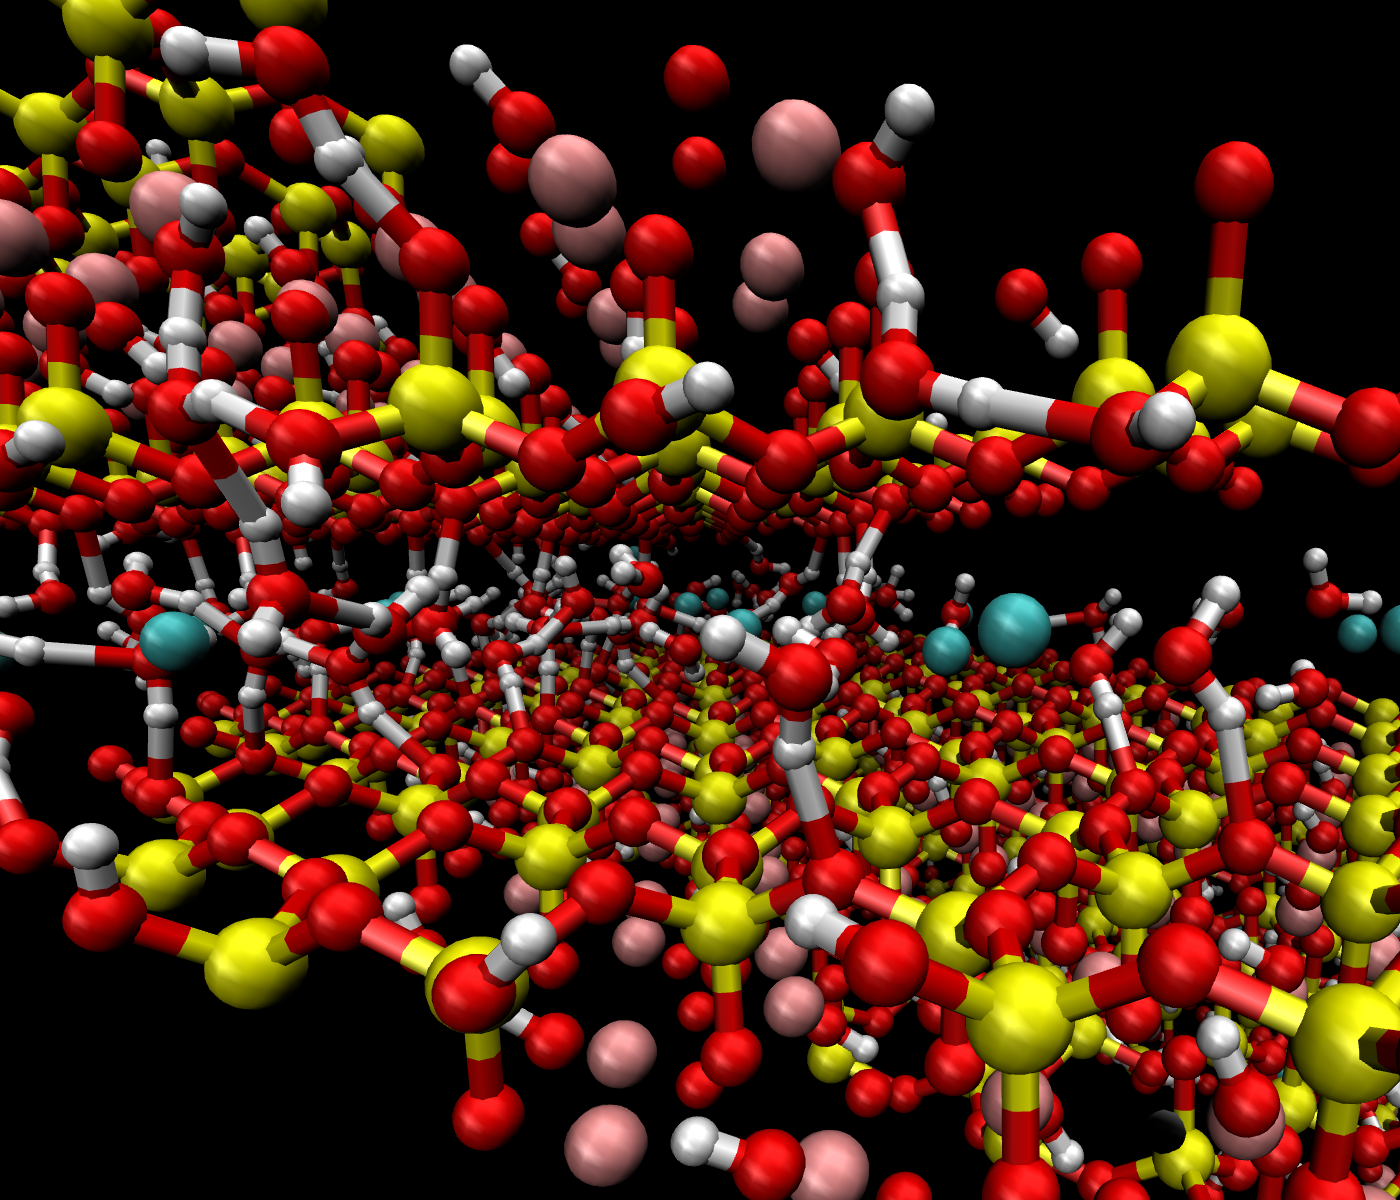
\includegraphics[scale=0.22]{images/mont_fin.png}
				\caption{Final state}
			\end{subfigure}
			\caption{VMD Visualizations of K montmorillonite sheet simulation.}
			\label{fig:mont_visual}
		\end{figure}
		
				
			
			


%%% Local Variables: 
%%% mode: latex
%%% TeX-master: t
%%% End:  % chapter 4
%%%%%%%%%%%%%%%%%%%%%%%%%%%%%%%%%%%%%%%%%%%%%%%%%%%%%%%%%%%%%%%%%%% 
%                                                                 %
%                            CHAPTER FIVE                         %
%                                                                 %
%%%%%%%%%%%%%%%%%%%%%%%%%%%%%%%%%%%%%%%%%%%%%%%%%%%%%%%%%%%%%%%%%%% 
 
\chapter{Conclusions and Future Considerations}
\section{Conclusions}
Through the course of this work, it was determined that saturated salt solutions provide a cheap plausible method for controlling the hydration levels of Li or Na montmorillonite samples in powder form. For these two species of exchangeable cation, a mono or bilayer hydrate should be attainable. It is not feasible however to hydrate clay samples in the form of compressed disks. Also noted is the fact that one has only a few minutes to conduct a measurement outside of the regulated environment of the desiccator before a homogeneous bilayer hydrate is reduced to a monolayer.

Infrared spectra of montmorillonite samples of varying exchangeable cation were obtained with pH values between 3 and 10. These spectra indicate that the frequency of the symmetric stretching mode of intercalated water is affected by the pH value, and as pH increases, so does the frequency of this vibrational mode. This was observed for samples of all species of exchangeable cation, and for samples coming from different clay mines as well. In general, most sample series examined experienced a shift in frequency of approximately 21 $cm^{-1}$ over the interval of pH 3 to pH 10. The frequency of the water deformation mode, and the O-H stretching mode of the structural hydroxyl groups did not appear to have any significant dependence on the pH. Also observed however was that while the frequency of the structural O-H stretching mode did not change with the pH, the value of this frequency seemed to be dependent on the clay mine from which it came, and not the species of interlaminar cation.

A model to simulate the molecular vibrations of water intercalated in montmorillonite is also provided, using the structures and force field provided with the InterfaceFF in combination with the flexible water model. The method used to calculate the vibrational frequencies is also detailed, where Fourier transforms are taken of the angle between H atoms, and their distances from the O atom. Using this technique with the described models, the frequencies observed experimentally through the infrared spectroscopic measurements were accurately reproduced in the molecular dynamics simulations. This will provide a foundation from which future simulations examining the pH effects may be based.

\section{pH Variations in Molecular Dynamics Simulations}
While a model was developed to accurately simulate and calculate the vibrational modes of water intercalated in montmorillonites, no method was proposed to vary the pH of this system. In order to further investigate the experimental results discussed in Chapter 3, a means of changing the pH of the system must be determined. There are likely two possibilities to accomplish this. The first option is where H$^+$ ions are added to the interlaminar region with the water, and are allowed to move about in the system.

Another approach which has been used previously in simulations of silica-water interfaces is to adjust the charges on the surface of the silica structure in a manner which reflects the different hydrogenation states which would occur with different pH levels \cite{emami2014force}, \cite{emami2014prediction}. This approach requires determining which atoms should receive a charge adjustment, and by what quantity. It must also be ensured that the system remains charge neutral as a whole. The next step should be the development of the process to apply this method to the montmorillonite samples, so that changes in the pH may be investigated using molecular dynamic simulations.

\section{Terahertz Spectroscopy}
While we have been considering interactions between the water molecules and the exchangeable cations and the surface of the clay structure, interactions between water molecules have not been adequately examined. The intercalated water molecules may form hydrogen bonds with one another, also affecting their intramolecular vibrational modes. One method of examining hydrogen bond networks is with terahertz spectroscopy \cite{liu1997terahertz}, \cite{shiraga2014hydration}. The first half of Equation~\ref{eq:potential} governing the intramolecular forces was probed using infrared spectroscopy. This is of course only half of the picture, and terahertz spectroscopy can help complete this picture, exploring the intermolecular forces which are described in the second half of Equation~\ref{eq:potential}. Such experiments could also be used to improve the model upon which the simulations have been based, providing better data for those who study clay minerals, and potential similar compounds such as silica and glass structures. Investigating the hydrogen bond density of the intercalated water would shine a new light on the questions at hand, as well as potentially help answer more general questions about the behavior of water confined on the nanoscale.

%%% Local Variables: 
%%% mode: latex
%%% TeX-master: t
%%% End: 
 % chapter 5
%%%%%%%%%%%%%%%%%%%%%%%%%%%%%%%%%%%%%%%%%%%%%%%%%%%%%%%%%%%%%%%%%%% 
%                                                                 %
%                           BIBLIOGRAPHY                          %
%                                                                 %
%%%%%%%%%%%%%%%%%%%%%%%%%%%%%%%%%%%%%%%%%%%%%%%%%%%%%%%%%%%%%%%%%%% 
 
%This method produces a numbered bibliography where the numbers
%correspond to the \cite commands in the text. See the LaTeX manual.
%
\specialhead{REFERENCES}
\bibliographystyle{IEEEtran.bst} % specify bibliography style
\begin{singlespace}
  \bibliography{references} % Prints the bibliography here, using "references.bib"
\end{singlespace}

% Note that, if you wish, you can use BibTeX to create your bibliography
% from a database. See section 5.6.2 of Memo RPI.110 for information. 
%%% Local Variables: 
%%% mode: latex
%%% TeX-master: t
%%% End: 
 % bibliography
%%%%%%%%%%%%%%%%%%%%%%%%%%%%%%%%%%%%%%%%%%%%%%%%%%%%%%%%%%%%%%%%%%%
%                                                                 %
%                            APPENDICES                           %
%                                                                 %
%%%%%%%%%%%%%%%%%%%%%%%%%%%%%%%%%%%%%%%%%%%%%%%%%%%%%%%%%%%%%%%%%%%
 
\appendix    % This command is used only once!
\addcontentsline{toc}{chapter}{APPENDICES}             %toc entry  or:
%\addtocontents{toc}{\parindent0pt\vskip12pt APPENDICES} %toc entry, no page #
\chapter{Example LAMMPS Input Cards}

\section{CVFF Input Card}
\label{appendix:cvff}
\begin{singlespace}
\begin{verbatim}
# structure info
boundary p p p
units real
dimension 3
atom_style full
kspace_style pppm 1.0e-6
pair_style lj/cut/coul/long 12.0 8.0
bond_style harmonic
angle_style harmonic
dihedral_style harmonic
improper_style cvff

# Read in montmorillonite data file
read_data Combined_Card.data

# Use Waldman-Hagler combination rule
pair_modify mix sixthpower

# set water group
group water type 16 17

kspace_style pppm 1.0e-6
neigh_modify delay 0 every 1 check yes

# Generate random velocities for all particles T=300K random seed 8746
velocity all create 300 8746

# set timestep
timestep 0.25
thermo 10
fix 2 all nve/limit 0.05
run 1000
unfix	2
fix 2 all npt temp 300 300 10 iso 1 1 100
run 2000
dump 1 water custom 1 waterData id type mol xu yu zu
dump 22 all xyz 100 posout.xyz
run 200000
\end{verbatim}
\end{singlespace}

\section{ReaxFF Input Card}
\label{appendix:reaxff}
\begin{singlespace}
\begin{verbatim}
# structure info
boundary p p p
%units real
dimension 3

# read data
atom_style full
read_data Kaolinite.data
pair_style reax/c NULL
pair_coeff * * ffield_CaSiAlO_Pitman.bin Al H O Si
velocity all create 300 8746

# set timestep
timestep 0.5
thermo 10
fix 1 all qeq/reax 1 0.0 10.0 1.0e-6 reax/c
fix 2 all nve/limit 0.05
dump 1 all xyz 10 posout.xyz
run 1000
unfix	2

fix 2 all npt temp 300 300 10 iso 1 1 100

run 1000

fix 3 all nve 
run 20000
\end{verbatim}
\end{singlespace}


\chapter{Codes Used For Analysis}

\section{Python Script for Fourier Filter and Peak Locator}
\label{appendix:fft_filter}
\begin{singlespace}
\begin{verbatim}
"""
    Fourier Filter
    Hunter Belanger - hunter.belanger@gmail.com
    Perform a FFT to remove high frequency noise from a signal stored
    in a csv file. Fitered signal also output to csv.
"""

# Imports -----------------------------------------------------
import peakutils
import numpy as np
from numpy import fft

# Functions ---------------------------------------------------
def Read_CSV(flnm):
    y = []
    x = []
    # Open file
    fl = open(flnm)
    # Read in data
    for line in fl:
        line = line.split(",")
        x.append(float(line[0]))
        y.append(float(line[1]))
    # Close file
    fl.close()
    
    return (x,y)

def RM_Background(y, linear=True):
    if linear:
        bg = np.arange(y[0], y[-1], (y[-1]-y[0])/float(len(y)))
        if len(bg) != len(y):
            print "Help"
            bg = bg[:-1]
        return y - bg
    
    else:
        bg = []
        for i in range(len(y)):
        bg.append(min(y))
        return np.array(y) - np.array(bg)

def FFT_Filter(x,y,frq):
    F = fft.rfft(y)
    frqs = fft.rfftfreq(len(y), (x[1]-x[0]))
    
    for i in range(len(F)):
        if frqs[i] >= frq:
        F[i] = 0

    y_out = fft.irfft(F)
    
    return y_out

def Write_CSV(x,y,z, flnm):
    fl = open(flnm, "w")

    for i in range(len(x)):
        line = str(x[i]) + "," + str(y[i]) + "," + str(z[i]) + "\n"
        fl.write(line)
    
    fl.close()

# Main --------------------------------------------------------
if __name__ == "__main__":
    flnm = raw_input("Enter File Name => ")
    
    # Read in data
    t,s = Read_CSV(flnm)
    
    wn = []
    ab = []
    
    # Only keep data above 2500 wavenumbers
    for i in range(len(t)):
        if t[i] >= 2500:
        wn.append(t[i])
        ab.append(s[i])
    
    # Removes last data point which is extraneous
    wn = wn[:-1]
    ab = ab[:-1]
    
    # Remove background
    ab = RM_Background(ab)
    
    # Perform Fourier Filter
    ab_out = FFT_Filter(wn,ab,0.024)
    
    # Send data to numpy arrays
    wn = np.array(wn)
    ab_out = np.array(ab_out)
    
    # Hydrx indecies
    lH = np.where( abs(wn - 3350) == min(abs(wn - 3350)))
    hH = np.where( abs(wn - 3450) == min(abs(wn - 3450)))
    
    # Wtr indecies
    lW = np.where( abs(wn - 3450) == min(abs(wn - 3450)))
    hW = np.where( abs(wn - 4000) == min(abs(wn - 4000)))
    
    # Gets Hydrx pk by fitting Gaussians
    pksH = peakutils.interpolate(wn[lH[0][0]:hH[0][0]], 
                                 ab_out[lH[0][0]:hH[0][0]])

    # Gets Hydrx pk by fitting Gaussians
    pksW = peakutils.interpolate(wn[lW[0][0]:hW[0][0]],
                                 ab_out[lW[0][0]:hW[0][0]])
    
    print pksH
    print pksW
    print pksW[0]
\end{verbatim}
\end{singlespace}

\newpage
\section{C++ Program to Obtain Vibrational Modes of Water Molecules}
\label{appendix:cpp_freqs}
\begin{singlespace}
\begin{verbatim}
/*
    Frequency Parser
    Hunter Belanger - hunter.belanger@gmail.com

    Compile: g++ -Ofast -lgsl -lgslcblas -lm -lfftw3 -Wall main.cpp -o main
    Run: ./main path/to/dump/file LAMMPS_Timestpe Data_Dumped_Every 
    (Eg: ./main waterData 0.25 1)
*/

#include <iostream>
#include <iomanip>
#include <math.h>
#include <string>
#include <fstream>
#include <vector>
#include <boost/algorithm/string.hpp>
#include <fftw3.h>
#include <gsl/gsl_rng.h>
#include <gsl/gsl_matrix.h>
#include <gsl/gsl_vector.h>
#include <gsl/gsl_blas.h>
#include <gsl/gsl_multifit_nlinear.h>

using namespace std;
using namespace boost::algorithm;

struct data {
    size_t n;
    double * t;
    double * y;
};

int expb_f (const gsl_vector * x, void *data, gsl_vector * f) {
    size_t n = ((struct data *)data)->n;
    double *t = ((struct data *)data)->t;
    double *y = ((struct data *)data)->y;

    double A = gsl_vector_get (x, 0);
    double x0 = gsl_vector_get (x, 1);
    double w = gsl_vector_get (x, 2);

    size_t i;

    for (i = 0; i < n; i++) {
        /* Model Yi = A * exp(-(t_i - x0)^2/w)*/
        double Yi = A * exp (- ((t[i] - x0)*(t[i] - x0))/w );
        gsl_vector_set (f, i, Yi - y[i]);
    }

    return GSL_SUCCESS;
}

int expb_df (const gsl_vector * x, void *data, gsl_matrix * J) {
    size_t n = ((struct data *)data)->n;
    double *t = ((struct data *)data)->t;

    double A = gsl_vector_get (x, 0);
    double x0 = gsl_vector_get (x, 1);
    double w = gsl_vector_get (x, 2);

    size_t i;

    for (i = 0; i < n; i++) {
        /* Jacobian matrix J(i,j) = dfi / dxj, */
        double e = exp(- (t[i] - x0)*(t[i] - x0)/w);
        gsl_matrix_set (J, i, 0, e);
        gsl_matrix_set (J, i, 1, A * e * (2*(t[i]-x0)/w));
        gsl_matrix_set (J, i, 2, A * e * ((t[i]-x0)*(t[i]-x0))/(w*w));
    }

    return GSL_SUCCESS;
}

void Numbers_From_File(char* &fname, int &ntsteps, int &natoms, 
                       int &minmol, int &maxmol) {
    ifstream dataFile(fname);
    string line;
    vector<string> lineV = vector<string>();
    int count = 0;
    int acount = 0;
    bool parse (false);
    while(getline(dataFile, line)) {
        count += 1;
        if (count == 4) {natoms = stoi(line);}

        if ((ntsteps == 1) and (parse)) {
            acount += 1;
            split(lineV, line, is_space());
            if (stoi(lineV[2]) < minmol) {minmol = stoi(lineV[2]);}
            else if (stoi(lineV[2]) > maxmol) {maxmol = stoi(lineV[2]);}

            if (acount == natoms) {parse = false;}
        }

        if (trim_copy(line) == "ITEM: ATOMS id type mol xu yu zu") {
            ntsteps += 1;
            parse = true;
        }
    }

    dataFile.close();
}

void Sort_Molecules(double** &data, double*** molecules, int* &H1, 
                    int* &H2, int* &O, int &tstep, int &natoms, 
                    int &minmol, int &maxmol) {
    double* rH1 = (double*) calloc(3, sizeof(double));
    double* rH2 = (double*) calloc(3, sizeof(double));
    double* rO = (double*) calloc(3, sizeof(double));
    double* r1 = (double*) calloc(3, sizeof(double));
    double* r2 = (double*) calloc(3, sizeof(double));
    int cnt = 0;
    for (int i = 0; i < (maxmol - minmol + 1); i++) {
        for (int atm = 0; atm < natoms; atm++) {
            if (data[atm][0] == H1[i]) {
                rH1[0] = data[atm][3];
                rH1[1] = data[atm][4];
                rH1[2] = data[atm][5];
                cnt += 1;
            }
            else if (data[atm][0] == H2[i]) {
                rH2[0] = data[atm][3];
                rH2[1] = data[atm][4];
                rH2[2] = data[atm][5];
                cnt += 1;
            }
            else if (data[atm][0] == O[i]) {
                rO[0] = data[atm][3];
                rO[1] = data[atm][4];
                rO[2] = data[atm][5];
                cnt += 1;
            }

            if (cnt == 3) {break;}
        }
        cnt = 0;
        r1[0] = rH1[0] - rO[0];
        r1[1] = rH1[1] - rO[1];
        r1[2] = rH1[2] - rO[2];

        r2[0] = rH2[0] - rO[0];
        r2[1] = rH2[1] - rO[1];
        r2[2] = rH2[2] - rO[2];

        double mr1 = pow( r1[0]*r1[0] + r1[1]*r1[1] + r1[2]*r1[2] ,0.5);
        double mr2 = pow( r2[0]*r2[0] + r2[1]*r2[1] + r2[2]*r2[2] ,0.5);

        r1[0] /= mr1;
        r1[1] /= mr1;
        r1[2] /= mr1;

        r2[0] /= mr2;
        r2[1] /= mr2;
        r2[2] /= mr2;

        double  theta = acos( r1[0]*r2[0] + r1[1]*r2[1] + r1[2]*r2[2] );

        // put values in molecules matrix
        molecules[i][0][tstep] = mr1;
        molecules[i][1][tstep] = mr2;
        molecules[i][2][tstep] = theta;
    }
}

void Get_IDs(double** &data, int* &H1, int* &H2, int* &O, int &natoms, 
             int &minmol, int &maxmol) {
    for (int nmol = minmol; nmol <= maxmol; nmol ++) {
        int idH1 = 0;
        int idH2 = 0;
        int idO = 0;
        int cnt = 0;
        for (int i = 0; i < natoms; i++) {
            if (nmol == data[i][2]) {
                if (data[i][1] == 18) {
                    idO = (int) data[i][0];
                    cnt += 1;
                }
                else {
                    if (idH1 == 0) {
                        idH1 = (int) data[i][0];
                        cnt += 1;
                    }
                    else {
                        idH2 = (int) data[i][0];
                        cnt += 1;
                    }
                }
            }

            if (cnt == 3) {break;}
        }
        H1[nmol - minmol] = idH1;
        H2[nmol - minmol] = idH2;
        O[nmol - minmol] = idO;
    }
}

void Get_Vibrations(char* &fname, double*** &molecules, int &natoms, 
                    int &nmol, int &minmol, int &maxmol) {
    // Arrays for atom ids
    int* H1 = (int*) calloc(nmol, sizeof(int));
    int* H2 = (int*) calloc(nmol, sizeof(int));
    int* O = (int*) calloc(nmol, sizeof(int));

    // Initial line string and vector for boost
    string line ("Initial String");
    vector<string> lineV = vector<string>();

    // Array for timestep data
    double** stepdata = (double**) calloc(natoms, sizeof(double*));
    for (int i = 0; i < natoms; i++) {
        stepdata[i] = (double*) calloc(6, sizeof(double));
    }

    // Open file
    ifstream dataFile(fname);
    bool parse (false);
    int tstep = 0;
    int acount = 0;
    // Go through all lines in file
    while (getline(dataFile, line)) {
        // If in data section of time step
        if (parse) {
            // Add atom data to stepdata array
            split(lineV, line, is_space());
            stepdata[acount][0] = stod(lineV[0]);
            stepdata[acount][1] = stod(lineV[1]);
            stepdata[acount][2] = stod(lineV[2]);
            stepdata[acount][3] = stod(lineV[3]);
            stepdata[acount][4] = stod(lineV[4]);
            stepdata[acount][5] = stod(lineV[5]);
            acount += 1;

            // If all atoms in timestep read
            if (acount == natoms) {
                parse = false;
                if (tstep == 0) {
                    Get_IDs(stepdata, H1, H2, O, natoms, minmol, maxmol);
                }
                Sort_Molecules(stepdata, molecules, H1, H2, O, tstep,
                               natoms, minmol, maxmol);
                tstep += 1;
                acount = 0;
            }
        }

        // If at beginning of timestep
        else if (trim_copy(line) == "ITEM: ATOMS id type mol xu yu zu") {
            parse = true;
        }
    }
}

double Fit_Peaks(double* &x_in, double* &y_in, int &low, int &high) {
    size_t n = high - low + 1;

    const gsl_multifit_nlinear_type *T = gsl_multifit_nlinear_trust;
    gsl_multifit_nlinear_workspace *w;
    gsl_multifit_nlinear_fdf fdf;
    gsl_multifit_nlinear_parameters fdf_params = 
	   gsl_multifit_nlinear_default_parameters();
    const size_t p = 3; // Number of parameters

    gsl_vector *f;
    //gsl_matrix *J;
    gsl_matrix *covar = gsl_matrix_alloc (p, p);
    double* t = (double*) calloc(n,sizeof(double));
    double* y = (double*) calloc(n,sizeof(double));
    double* weights = (double*) calloc(n,sizeof(double));
    struct data d = {n, t, y};

    // Inital values based on which peak
    double x_init[3] = {0, 0, 0};
    if (x_in[low] < 1400) {
        x_init[0] = 0.4;
        x_init[1] = 1440.0;
        x_init[2] = 3400.0;
    }
    else if (x_in[low] < 3600) {
        x_init[0] = 0.8;
        x_init[1] = 3610.0;
        x_init[2] = 1000.0;
    }
    else {
        x_init[0] = 0.8;
        x_init[1] = 3670.0;
        x_init[2] = 1000.0;
    }
    gsl_vector_view x = gsl_vector_view_array (x_init, p);
    gsl_vector_view wts = gsl_vector_view_array(weights, n);
    gsl_rng * r;
    //double chisq;
    double chisq0;
    int info;
    size_t i;

    const double xtol = 1e-8;
    const double gtol = 1e-8;
    const double ftol = 0.0;

    gsl_rng_env_setup();
    r = gsl_rng_alloc(gsl_rng_default);

    /* define the function to be minimized */
    fdf.f = expb_f;
    fdf.df = expb_df;   /* set to NULL for finite-difference Jacobian */
    fdf.fvv = NULL;     /* not using geodesic acceleration */
    fdf.n = n;
    fdf.p = p;
    fdf.params = &d;

    // Define data to be fitted
    for (i = 0; i < n; i++) {
        t[i] = x_in[low+i];
        y[i] = y_in[low+i];
        weights[i] = 1.0;
    }

    /* allocate workspace with default parameters */
    w = gsl_multifit_nlinear_alloc (T, &fdf_params, n, p);

    /* initialize solver with starting point and weights */
    gsl_multifit_nlinear_winit (&x.vector, &wts.vector, &fdf, w);

    /* compute initial cost function */
    f = gsl_multifit_nlinear_residual(w);
    gsl_blas_ddot(f, f, &chisq0);

    /* solve the system with a maximum of 1000 iterations */
    gsl_multifit_nlinear_driver(1000, xtol, gtol, ftol, NULL, NULL, &info, w);

    // Get frequency from fitted parameters
    double x0 = gsl_vector_get(w->x,1);

    gsl_multifit_nlinear_free (w);
    gsl_matrix_free (covar);
    gsl_rng_free (r);

    return x0;
}

void Get_Frequencies(double*** &molecules, vector<double> &fWl, 
                     vector<double> &fWh, vector<double> &fTheta, 
                     double &tstep, int &ntsteps, int &nmols) {
    // Initialize frequency array to used for fitting
    int n_out = (ntsteps/2) + 1;
    double c = 29979245800.0;
    double* freq = (double*) calloc(n_out, sizeof(double));
    int thLow = 0;
    int thHigh = 0;
    int w1Low = 0;
    int w1High = 0;
    int w2High = 0;
    for (int i = 0; i < n_out; i++) {
        freq[i] = (double)i / (tstep*n_out*2);
        freq[i] /= c;
    }

    for (int i = 0; i < n_out; i++) {
        // Get indicies for fitting locations
        if ((freq[i] < 1200) and (freq[i+1] > 1200)) {thLow = i;}
        else if ((freq[i] < 1700) and (freq[i+1] > 1700)) {thHigh = i+1;}

        else if ((freq[i] < 3450) and (freq[i+1] > 3450)) {w1Low = i;}
        else if ((freq[i] < 3625) and (freq[i+1] > 3625)) {w1High = i+1;}

        else if ((freq[i] < 3700) and (freq[i+1] > 3700)) {w2High = i+1;}
    }

    // Go get FFT and peaks for all molecules
    for (int i = 0; i < nmols; i++) {
        // Define input vectors of real values
        double* inr1 = molecules[i][0];
        double* inr2 = molecules[i][1];
        double* inTh = molecules[i][2];

        // Get averages and remove
        double r1avg = 0;
        double r2avg = 0;
        double thtavg = 0;
        for (int j = 0; j < ntsteps; j++) {
            r1avg += inr1[j];
            r2avg += inr2[j];
            thtavg += inTh[j];
        }
        r1avg /= (double) ntsteps;
        r2avg /= (double) ntsteps;
        thtavg /= (double) ntsteps;
        for (int j = 0; j < ntsteps; j++) {
            inr1[j] -= r1avg;
            inr2[j] -= r2avg;
            inTh[j] -= thtavg;
        }


        // Output vectors for complex values
        fftw_complex* outr1 = 
            (fftw_complex*)fftw_malloc(sizeof(fftw_complex)*n_out);
        fftw_complex* outr2 = 
            (fftw_complex*)fftw_malloc(sizeof(fftw_complex)*n_out);
        fftw_complex* outTh = 
            (fftw_complex*)fftw_malloc(sizeof(fftw_complex)*n_out);

        // Define FFT plan for the three functions
        fftw_plan planr1, planr2, planTh;
        planr1 = fftw_plan_dft_r2c_1d(ntsteps, inr1, outr1, FFTW_ESTIMATE);
        planr2 = fftw_plan_dft_r2c_1d(ntsteps, inr2, outr2, FFTW_ESTIMATE);
        planTh = fftw_plan_dft_r2c_1d(ntsteps, inTh, outTh, FFTW_ESTIMATE);

        // Perform FFT
        fftw_execute(planr1);
        fftw_execute(planr2);
        fftw_execute(planTh);

        // Destroy previous plans and in/outs
        fftw_destroy_plan(planr1);
        fftw_destroy_plan(planr2);
        fftw_destroy_plan(planTh);

        // Arrays for frequency magnitudes
        double* magr1 = (double*) calloc(n_out, sizeof(double));
        double* magr2 = (double*) calloc(n_out, sizeof(double));
        double* magth = (double*) calloc(n_out, sizeof(double));

        double maxr1 = 0;
        double maxr2 = 0;
        double maxth = 0;
        // Add magnitudes to arrays
        for (int j = 0; j < n_out; j++) {
            magr1[j] = pow( outr1[j][0]*outr1[j][0] + 
                            outr1[j][1]*outr1[j][1] ,0.5);
            if (magr1[j] > maxr1) {maxr1 = magr1[j];}
            magr2[j] = pow( outr2[j][0]*outr2[j][0] + 
                            outr2[j][1]*outr2[j][1] ,0.5);
            if (magr2[j] > maxr2) {maxr2 = magr2[j];}
            magth[j] = pow( outTh[j][0]*outTh[j][0] + 
                            outTh[j][1]*outTh[j][1] ,0.5);
            if (magth[j] > maxth) {maxth = magth[j];}
        }
        // Normalize arrays
        for (int j = 0; j < n_out; j++) {
            magr1[j] /= maxr1;
            magr2[j] /= maxr2;
            magth[j] /= maxth;
        }

        // Fit curves and get frequencies
        double freqTht = Fit_Peaks(freq, magth, thLow, thHigh);
        if ( (freqTht < 1700) and (freqTht > 1200) ) 
        {fTheta.push_back(freqTht);}

        double freqLow = Fit_Peaks(freq, magr1, w1Low, w1High);
        if ( (freqLow < 3625) and (freqLow > 3450) ) 
        {fWl.push_back(freqLow);}

        freqLow = Fit_Peaks(freq, magr2, w1Low, w1High);
        if ( (freqLow < 3625) and (freqLow > 3450) ) 
        {fWl.push_back(freqLow);}

        double freqHigh = Fit_Peaks(freq, magr1, w1High, w2High);
        if ( (freqHigh < 3700) and (freqHigh > 3625) ) 
        {fWh.push_back(freqHigh);}

        freqHigh = Fit_Peaks(freq, magr2, w1High, w2High);
        if ( (freqHigh < 3690) and (freqHigh > 3650) ) 
        {fWh.push_back(freqHigh);}

        fftw_free(outr1);
        fftw_free(outr2);
        fftw_free(outTh);
    }
}

int main (int argc, char* argv[]) {
    double timestep = stod(argv[2]);
    double outputstep = stod(argv[3]);

    // Get number of atoms and timesteps
    int ntimesteps = 0;
    int natoms = 0;
    int minmol = 1000000;
    int maxmol = 0;
    cout << "Getting numbers...\n";
    Numbers_From_File( argv[1], ntimesteps, natoms, minmol, maxmol);
    cout << "Ntimesteps:" << ntimesteps << " " << "Natoms:" << natoms 
         << " " << "MinMol:" << minmol << " " << "MaxMol:" << maxmol << "\n\n";
    int nmol = maxmol - minmol +1;

    // Initialize array for data to be transformed
    double*** moleculeData = (double***) calloc(nmol, sizeof(double**));
    for (int i = 0; i < nmol; i++) {
        moleculeData[i] = (double**) calloc(3, sizeof(double*));
        for (int j = 0; j < 3; j++) {
            moleculeData[i][j] = (double*) calloc(ntimesteps, sizeof(double));
        }
    }

    // Get molecule data
    cout << "Geting atom data...\n\n";
    Get_Vibrations(argv[1], moleculeData, natoms, nmol, minmol, maxmol);

    cout << "Doing Fourier transforms...\n\n";
    vector<double> fTheta = vector<double>();
    vector<double> fWl = vector<double>();
    vector<double> fWh = vector<double>();
    double tstep = timestep*outputstep*(1E-15); // Convert to s
    Get_Frequencies(moleculeData, fWl, fWh, fTheta, tstep, ntimesteps, nmol);


    // Calculate average frequencies
    double thavg = 0;
    double wlavg = 0;
    double whavg = 0;

    for (size_t i = 0; i < fTheta.size(); i++) {
        thavg += fTheta[i];
    }
    thavg /= (double) fTheta.size();

    for (size_t i = 0; i < fWl.size(); i++) {
        wlavg += fWl[i];
    }
    wlavg /= (double) fWl.size();

    for (size_t i = 0; i < fWh.size(); i++) {
        whavg += fWh[i];
    }
    whavg /= (double) fWh.size();

    // Calculate standard deviations
    double thstd = 0;
    double wlstd = 0;
    double whstd = 0;
    for (size_t i = 0; i < fTheta.size(); i++) {
        thstd += pow( thavg - fTheta[i] ,2);
    }
    thstd /= ((double) fTheta.size() - 1.0);
    thstd = pow(thstd, 0.5);

    for (size_t i = 0; i < fWl.size(); i++) {
        wlstd += pow( wlavg - fWl[i] ,2);
    }
    wlstd /= ((double) fWl.size() - 1.0);
    wlstd = pow(wlstd, 0.5);

    for (size_t i = 0; i < fWh.size(); i++) {
        whstd += pow( whavg - fWh[i] ,2);
    }
    whstd /= ((double) fWh.size() - 1.0);
    whstd = pow(whstd, 0.5);

    // Print averages
    cout << fixed;
    cout << setprecision(3);
    cout << "Tht:   " << thavg << " +/- " << thstd << "\n";
    cout << "Wlow:  " << wlavg << " +/- " << wlstd << "\n";
    cout << "Whigh: " << whavg << " +/- " << whstd << "\n\n";
        
    return 0;
}
\end{verbatim}
\end{singlespace}

\chapter{Supplemental Files}
The supplemental file JACS\_Reuse\_Permission.jpg (252.6 kB), is a jpeg image of the permissions for the reuse of Figure~\ref{fig:clay_structure} in this thesis.
 
 % appendix
 
\end{document}
